\documentclass[reprint,prb,superscriptaddress]{revtex4-2}
\usepackage{braket,amsmath,amssymb,graphicx,float,hyperref,color,ulem,soul,lipsum}
\allowdisplaybreaks
\bibliographystyle{apsrev4-2}
\begin{document}

\title{Supplementary Materials of ....}
\author{Siddhartha Patra}
% \email{mukherjee.anirban.anirban@gmail.com }
\affiliation{Department of Physical Sciences, Indian Institute of Science Education and Research-Kolkata, W.B. 741246, India}
\author{Abhirup Mukherjee}
\email{am18ip014@iiserkol.ac.in }
\affiliation{Department of Physical Sciences, Indian Institute of Science Education and Research-Kolkata, W.B. 741246, India}
\author{Anirban Mukherjee}
\email{mukherjee.anirban.anirban@gmail.com }
\affiliation{Department of Physical Sciences, Indian Institute of Science Education and Research-Kolkata, W.B. 741246, India}
\author{A. Taraphder}
\affiliation{Department of Physics, Indian Institute of Technology Kharagpur, Kharagpur 721302, India}
\author{Siddhartha Lal}
\email{slal@iiserkol.ac.in}
\affiliation{Department of Physical Sciences, Indian Institute of Science Education and Research-Kolkata, W.B. 741246, India}
\date{\today}
\begin{abstract}
	\lipsum[1-2]
\end{abstract}
\maketitle

\tableofcontents

%\section{Introduction}


%\section{Fixed point theory of over-screened MCK model}

%\subsection{RG flows towards intermediate coupling}
%\label{rg_flow_section}
%%We start with the usual \(K\)-channel Kondo model Hamiltonian with isotropic couplings \cite{Noz_blandin_1980}:
%%\begin{gather}
%%	\label{mc_ham}
%%	H = \sum_{l=1}^K H_l~,\nonumber\\
%%	H_l = \sum_{k}\sum_{\alpha=\uparrow,\downarrow}\epsilon_{k,l} \hat n_{k\alpha,l} + J\sum_{kk^\prime} \sum_{\alpha,\beta= \uparrow,\downarrow}\vec{S_d}\cdot\frac{1}{2}\vec{\sigma}_{\alpha\alpha^\prime}c_{k\alpha,l}^\dagger c_{k^\prime\alpha^\prime, l}~.
%%\end{gather}
%%Here, \(l\) sums over the \(K\) channels of the conduction bath, \(k,k^\prime\) sum over all the momentum states of the bath and \(\alpha,\beta\) sum over the two spin indices of a single electron. \(c_{k\alpha,l}\) is the fermionic field operator at momentum \(k\), spin \(\alpha\) and channel \(l\). \(\epsilon_{k,l}\) represents the dispersion of the \(l^\text{th}\) conduction channel. \(\vec \sigma\) is the vector of Pauli matrices and \(\vec S_d = \frac{1}{2}\vec \sigma_d\) is the impurity spin operator.
%%
%%We have performed a renormalisation group analysis of the Hamiltonian using the recently developed URG method \cite{anirbanmott2,anirbanmott2,anirbanurg1,anirbanurg2,siddharthacpi,santanukagome,1dhubjhep}. The RG proceeds \textit{by applying unitary transformations in order to block-diagonalize the Hamiltonian by removing number fluctuations of the high energy degrees of freedom}. If the most energetic electronic state at the \(j^\text{th}\) RG step is \(\ket{j}\) defined by the energy \(D_{(j)}\), the Hamiltonian will in general not conserve the number of particles in this state: \(\left[H_{(j)}, \hat n_{j}\right] \neq 0\). The unitary transformation \(U_{(j)}\) will remove this number fluctuation at the next RG step:
%%\begin{equation}\begin{aligned}
%%	H_{(j-1)} = U_{(j)} H_{(j)} U^\dagger_{(j)}, ~\left[H_{(j-1)}, \hat n_{j}\right] =0
%%\end{aligned}\end{equation}
%%The unitary transformations are given in terms of a fermionic generator \(\eta_{(j)}\):
%%\begin{equation}\begin{aligned}
%%	U_{(j)} = \frac{1}{\sqrt 2}\left(1 + \eta_{(j)} - \eta_{(j)}^\dagger\right), \quad\left\{ \eta_{(j)},\eta_{(j)}^\dagger \right\}_\pm = 1
%%\end{aligned}\end{equation}
%%where \(\left\{A,B\right\}_\pm = AB \pm BA\). The generator itself is given by the expression
%%\begin{equation}\begin{aligned}
%%	\eta^\dagger_{(j)} = \frac{1}{\hat \omega_{(j)} - \text{Tr}\left(H_{(j)} \hat n_{j}\right) } c^\dagger_{j} \text{Tr}\left(H_{(j)}c_{j}\right)
%%\end{aligned}\end{equation}
%%The operator \(\hat \omega_{(j)}\) encodes the quantum fluctuation scales arising from the interplay of the kinetic energy terms and the interaction terms of the Hamiltonian:
%%\begin{equation}\begin{aligned}
%%	\hat \omega_{(j)} = H_{(j-1)} - H^i_{(j)}
%%\end{aligned}\end{equation}
%%\(H^i_{(j)}\) is that part of \(H_{(j)}\) that commutes with \(\hat n_j\) but does not commute with at least one \(\hat n_l\) for \(l < j\). The RG continues up to energy \(D^*\) where a fixed point is reached from the vanishing of either the numerator or the denominator.
%%
%%The derivation of the RG equation for the over-screened regime \((2S < K)\) of the spin-\(S\)-impurity \(K\)-channel Kondo problem is shown in appendix \ref{appendix_urg}. On decoupling circular isoenergetic shells at energies \(D_{(j)}\), the change in the Kondo coupling at the \(j^\text{th}\) RG step, \(\Delta J_{(j)}\), is given by
%%\begin{equation}\begin{aligned}
%%	\Delta J_{(j)} = -\frac{J_{(j)}^2 \mathcal{N}_{(j)}}{\omega_{(j)} - \frac{D_{(j)}}{2} + \frac{J_{(j)}}{4}}\left( 1 - \frac{1}{2}\rho J_{(j)} K \right) 
%%\end{aligned}\end{equation}
%%\(\mathcal{N}_{(j)}\) is the number of electronic states at the energy shell \(D_{(j)}\). We work in the low quantum fluctuation regime \(\omega_{(j)} < \frac{D_{(j)}}{2}\). There are three fixed points of the RG equation. One arises from the vanishing of the denominator, and was present in the single-channel Kondo RG equation as well \cite{kondo_urg}. As shown there, this fixed-point goes to \(J^* = \infty\) as the bare bandwidth of the conduction electrons is made large. The other trivial fixed point is the trivial one at \(J^* = 0\). The third fixed point is reached when the numerator vanishes: \(J^* = \frac{2}{K \rho}\) \cite{Gan_mchannel_1994,Kogan_2018,Kuramoto1998,Noz_blandin_1980}. Only the intermediate fixed point is found to be stable. This is consistent with results from Bethe ansatz calculations~\cite{Tsvelick_Weigmann_mchannel_1984,andrei_destri_1984,zarand_costi_2002,andrei_jerez_1995,Tsvelick_1985,Tsvelick1984}, CFT calculations~\cite{affleck_1991_overscreen,affleck1993exact,affleck_ludwig_1991}, bosonization treatments~\cite{emery_kivelson,vondelft_prl_1998} and NRG analysis~\cite{pang_cox_1991,mitchell_bulla_2014}.
%%\begin{figure}[htpb]
%%	\centering
%%	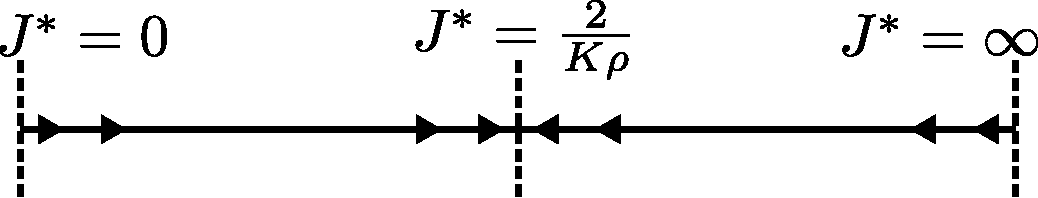
\includegraphics[width=0.45\textwidth]{plt/rg_flow.pdf}
%%	\caption{The three fixed points of the over-screened RG equation. Only the intermediate one is stable.}
%%	\label{rg_flow}
%%\end{figure}
%%
%%The RG equation reduces to the perturbative form \(\Delta J_{(j)} \simeq \frac{J_{(j)}^2 \mathcal{N}_{(j)}}{D_{(j)}}\left( 1 - \frac{1}{2}\rho J_{(j)} K \right)\)~\cite{Kogan_2018,Kuramoto1998,Noz_blandin_1980,tripathi2018landau} when one replaces \(\omega_{(j)}\) with the ground state energy \(-\frac{D_{(j)}}{2}\) and assumes \(J \ll D_{(j)}\).
%%
%%\subsection{Star graph as the effective fixed point Hamiltonian}
%%The fixed point Hamiltonian takes the form
%%\begin{equation}\begin{aligned}
%%	H^* = \sum_l\left[ \sum^*_{k}\epsilon_{k,l} \hat n_{k\alpha,l} + J\sum_{kk^\prime}^* \vec{S_d}\cdot\frac{1}{2}\vec{\sigma}_{\alpha\alpha^\prime}c_{k\alpha,l}^\dagger c_{k^\prime\alpha^\prime, l}~.\right]
%%\end{aligned}\end{equation}
%%We have not explicitly written the decoupled degrees of freedom \(D_{(j)} > D^*\) in the Hamiltonian. The \(*\) over the summations indicate that only the momenta inside the window \(D^*\) enter the summation. There is an implied summation over the spin indices \(\alpha,\beta\).
%%
%%To study the low energy physics and universality of the problem, we will mostly focus on the zero bandwidth limit of the fixed point Hamiltonian. Upon setting the chemical potential equal to the Fermi energy, this zero bandwidth model becomes a Heisenberg spin-exchange Hamiltonian.
%%\begin{equation}\begin{aligned}
%%	\label{stargraph}
%%	H^* = J\sum_l\sum_{kk^\prime}^* \vec{S_d}\cdot\frac{1}{2}\vec{\sigma}_{\alpha\alpha^\prime}c_{k\alpha,l}^\dagger c_{k^\prime\alpha^\prime, l} = J\vec{S_d}\cdot\sum_l \vec{s}_l~.
%%\end{aligned}\end{equation}
%%At the last step, we defined the local spin operator \(\vec{s}_l = \frac{1}{2}\sigma_l = \frac{1}{2}\sum_{kk^\prime}^*\sum_{\alpha\beta}\vec{\sigma}_{\alpha\alpha^\prime}c_{k\alpha,l}^\dagger c_{k^\prime\alpha^\prime, l}\) of each conduction channel.
%%\begin{figure}[htpb]
%%	\centering
%%	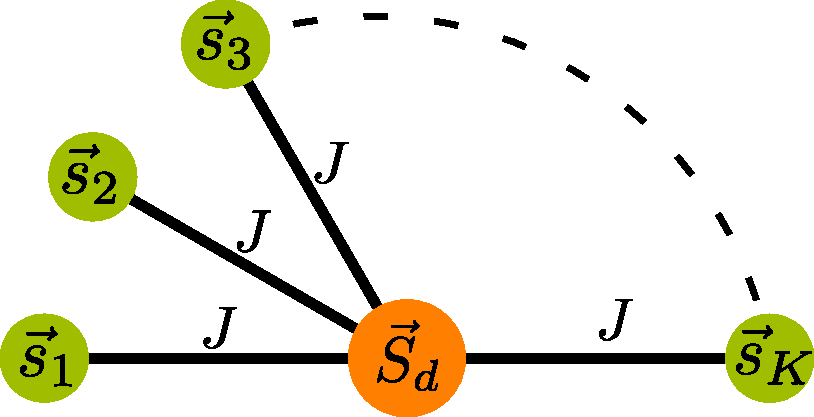
\includegraphics[width=0.30\textwidth]{plt/stargraph.pdf}
%%	\caption{Zero bandwidth limit of the fixed point Hamiltonian. The central yellow node is the impurity spin, which is talking withe the local spins of the channels represented as green nodes.}
%%	\label{fig:-stargraph-pdf}
%%\end{figure}
%%The star graph commutes with several operators, including the total spin operator \(J^z = S_d^z + \sum_l s_l^z\) along \(z\), the total bath local spin operator \(s^2_\text{tot} = \left(\sum_l \vec s_l\right)^2\) and the string operators 
%%\begin{equation}\begin{aligned}
%%\pi^{x,y,z} = \sigma_d^{x,y,z} \otimes_{l=1}^K \sigma_l^{x,y,z}~.
%%\end{aligned}\end{equation}
%%The \(\pi^z\) acts on the eigenstates \(\ket{J^z}\) and reveals the odd-even parity of the eigenvalue \(J^z\), and is hence a parity operator. Interestingly, \textit{the string operator \(\pi^z\) is a Wilson loop operator~\cite{fradkin2013field} that wraps around all the nodes of the star graph}:
%%\begin{equation}\begin{aligned}
%%	\label{w_loop}
%%	\pi^z = \exp\left[i \frac{\pi}{2} \left(\sigma_d^z + \sum_{l=1}^K \sigma^z_l - K\right)\right] = e^{i \pi \left(J^z - \frac{1}{2}K\right)}
%%\end{aligned}\end{equation}
%%\(\pi^x\) and \(\pi^y\) mix states of opposite parity. For example, it can be shown that \(\pi^x \ket{J^z} = -\ket{J^z}\). These are 't Hooft operators \cite{fradkin2013field}.
%%
%%
%%There are multiple reasons for working with the star graph in particular and zero mode Hamiltonians in general. In the single-channel Kondo model, the star graph is just the two spin Heisenberg, and it reveals the stabilization of the Kondo model ground state, as well as certain thermodynamic properties (e.g., the impurity contribution to the susceptibility)~\cite{varma_yafet_1976,yosida_1966,wilson1975renormalization,moca_zarand_2021,varma_yafet_1976,kondo_urg}. Similarly in the MCK model, the star graph is able to mimic the nature of the RG flows: At weak coupling \(J \to 0^+\), the central spin is weakly coupled to the outer spins and  prone to screening because of the \(s^\pm\) terms in the star graph, and at strong coupling \(J \to \infty^-\), the outer spin-half objects tightly bind with the central spin-half object to form a single spin object that interacts with the remaining states through an exchange coupling which is RG relevant, rendering both the terminal fixed points unstable. The true stable fixed point must then lie somewhere in between, and we recover the schematic phase diagram of fig.~\ref{rg_flow}. 
%%
%%The utility of the star graph is due to the fact that \textit{the non-Fermi liquid arises solely from the degeneracy of the ground state manifold of the underlying zero mode Hamiltonian, and the star graph captures this degeneracy in its entirety}. The RG flows of the MCK model have been show to \textit{preserve the degeneracy of the ground state}~\cite{pang_cox_1991,kroha_kolf_2007,zitko_fabrizio_2017}\textcolor{red}. The star graph conserves the total spin \(J^z\), and this leads to a ground state degeneracy of \(|\frac{K}{2}-S|+1\) in the \(K-\)channel spin-\(S\) star graph which is preserved under the RG flow. This is qualitatively different from the case of the single-channel Kondo model where the \(2-\)fold degeneracy of the local moment fixed point crosses over into a stable and unique singlet ground state. 
%%
%%As we will see in a subsequent section, the lowest excitations of the intermediate fixed point is described a non-Fermi liquid phase induced by nearest-neighbour hopping terms between the zeroth sites and the first sites of the conduction channels. The importance of the degeneracy can be shown in the following manner. As mentioned previously, the ground state degeneracy of the more general star graph with a spin-\(S\) impurity and \(K\) channels is given by \(g^S_K = |K - 2S|+1\). The cases of \(K=2S\), \(K<2S\) and \(K>2S\) correspond to exactly screened, under-screened and over-screened regimes respectively. \textit{The latter two cases correspond to a multiply-degenerate manifold \(g^S_K > 1\), and simultaneously have non-Fermi liquid phases~\cite{Noz_blandin_1980,Gan_Andrei_Coleman_1993,emery_kivelson,Gan_mchannel_1994,Tsvelick_Weigmann_mchannel_1984,Tsvelick_weigmann_mchannel_1985,parcollet_olivier_large_N,kimura_taro_Su_N_kondo,PhysRevB.73.224445,cox_jarrell_two_channel_rev,affleck_1991_overscreen,Coleman_tsvelik,affleck1993exact,coleman_pepin_2003,roch_nicolas_costi_2009,schiller_avraham_2008,Durganandini_2011}, while the first regime has a unique ground state \(g^S_K = 1\) and is described by a local Fermi liquid (LFL) phase \cite{wilson1975,nozieres1974fermi,Noz_blandin_1980,andreiKondoreview,tsvelickKondoreview}, thereby substantiating the claim that a degeneracy greater than unity leads to non-Fermi liquid physics.} In the following sections, we will show how the inherent quantum-mechanical frustration of singlet order that is present in the Hamiltonian leads to the degenerate ground state manifold and the non-trivial physics of the fixed points in terms of non-Fermi liquid phase, diverging thermodynamic quantities, quantum criticality as well as emergent gauge theories.
\section{Additional Properties of the Star Graph}
%\subsection{Hamiltonian and wavefunctions}
%\noindent As shown in the previous section, at the heart of multi channel Kondo there is a stargraph problem whic is the zero mode of the lowenergy fixed point Hamiltonian of the Multi channel Kondo. In this section our focus will be on the stargraph problem itself.
%\begin{figure}[!h]
%\centering
%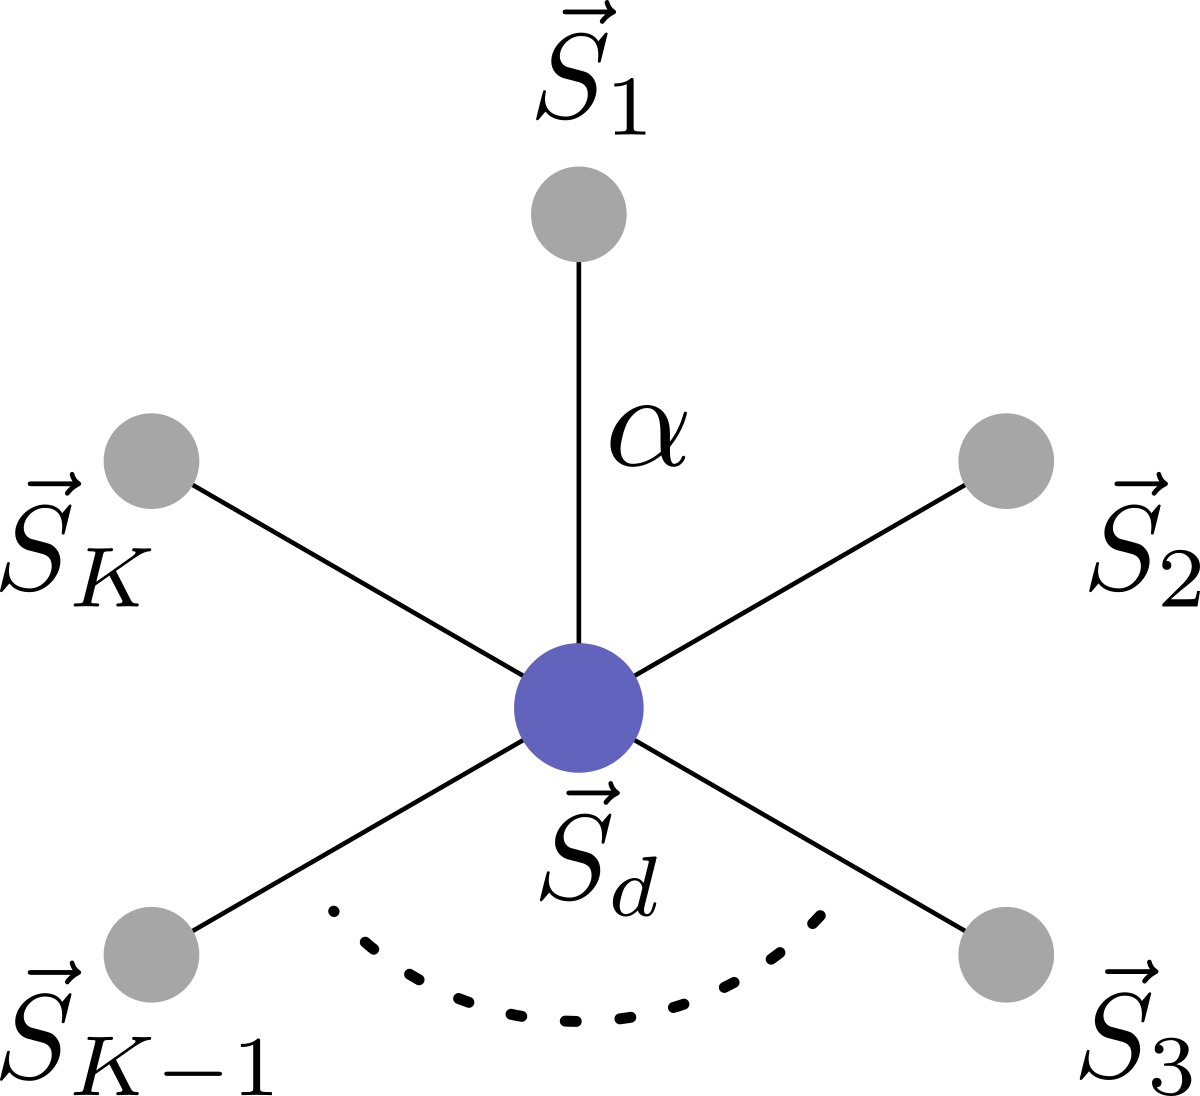
\includegraphics[scale=0.4]{plt/stargraph_first}
%\caption{This is a stargraph model with one central spin $\vec{S}_d$ and $K$ outer spin $1/2$s. The central spin is coupled with all the outer spins with Heisenberg coupling with coupling strength $\alpha$.}
%\label{fig:stargraph_first}
%\end{figure}
%As shown in the Fig.\ref{fig:stargraph_first} above one central spin ($\vec{S}_d$) is connected with $K$ spins forming a $K$ channel stargraph problem corresponding to the $K$-channel Kondo problem. The Hamiltonian of this above model is given as 
%\begin{eqnarray}
%H &=& \alpha \vec{S}_d.\sum_{i=1}^{K}\vec{S}_i=\alpha \vec{S}_d.\vec{S} \nonumber\\
%&=& \frac{\alpha}{2} (\vec{J}^2-\vec{S}^2-\vec{S}_d^2)~,~~\alpha >0.
%\label{eq:stargraph_hamiltonian}
%\end{eqnarray}
%where $\vec{J}=\vec{S}+\vec{S}_d$ and $\vec{S}=\sum_{i=1}^{K} \vec{S}_i$. One can see that the large psin $S$ can take many possible values as this is made out of $K$ spin 1/2s. We can see $[H,J]=0=[H,J^i]$ for  $i=x,y,z$, $[J^i,J^j]\neq 0$ for $i\neq j$. In our model we find two string operators $\hat{\mathbb{Z}}=\sigma_d^z\Pi_{i=1}^{K} \sigma_i^z$ and $\hat{\mathbb{X}}=\sigma_d^x\Pi_{i=1}^{K} \sigma_i^x$, where $K$ is the number of channels. These two operators commutes with the Hamiltonian $H$ of this stargraph.
%\begin{eqnarray}
%[H,\hat{\mathbb{Z}}] &=& 0 = [H,\hat{\mathbb{X}}]
%\end{eqnarray}
%We can rewrite the operators in the form of a twist operator as, $\mathbb{Z}=e^{i\pi [J^z-(\frac{K+1}{2})]}$ and $\mathbb{X}=e^{i\pi [J^x-(\frac{K+1}{2})]}$
%The commutation between these two operators are given as
%\begin{eqnarray}
%[\mathbb{Z},\mathbb{X}] &=& \prod_{i=d,1}^{K} \sigma^z_{i} \prod_{i=d,1}^{K} \sigma^x_{i} \bigg[1-(-1)^{K+1}\bigg]
%\end{eqnarray}
%Thus we can see that for case where number of channels is odd that means $K+1$ is even, these two string operators commutes with each other forming a CSCO ($H,\hat{\mathbb{Z}},\hat{\mathbb{X}}$). On the other hand in the case where number of channels $K$ is even, these two operators does not commute with each other. Thus we can form the CSCO with $H,J,J^z,S,S_d$. For a particular value $S$, $J$ can take two values $S\pm S_d$ with the energies $-\alpha S_d(S_d+1\mp J)$ respectively. $S_d$ is fixed thus the energy values only depends on the corresponding $J$ value of the state. As the energy does not depends on the $J^z$, all $2J+1$ $J^z$ states labeled by $|S_d,S;J,J^z\rangle$ are degenerate. It is easy to see that the ground state has energy $E=-\alpha S_d(S_d+1+J)$ with  $J=S-S_d$, thus $E_g=-\alpha S_d(S_{max}+1)$ with $S$ taking the maximum possible value $S_{max}=K/2$.
%
%
%\subsubsection{Ground state wavefunction}
%\noindent Above calculations show stargraph with $K$ channels has $K$-fold ground state degeneracy, states labeled as $|S_d,S;J,J^z\rangle$ where $J^z$ takes $K=2J+1$ distinct values, $J^z=\{-J,\cdots,+J \}$. Here our goal is to find the wavefunction in the fundamental spin basis $|S_d^z,S_1^z,\cdots,S_K^z\rangle$. To achieve that we use the Clebsch-gordon coefficients, we know for two spins $j_1$ and $j_2$  with total spin $J$ and $J^z=M$ one can expand the state as 
%\begin{eqnarray}
%|j_1,j_2;J,M\rangle &=& \displaystyle\sum_{\substack{m_1=\{-j_1,\cdots,j_1\} \\ m_2=\{-j_2,\cdots,j_2\} }}   \mathcal{C}^{j_1,m_1;j_2,m_2}_{j_1,j_2;J,M} |j_1,m_1;j_2,m_2 \rangle ,~~~~
%\end{eqnarray}
%where $j_1^z=m_1$ and $j_2^z=m_2$ and $\mathcal{C}^{j_1,m_1;j_2,m_2}_{j_1,j_2;J,M}$ is the Clebs-Gordon coefficient. In our problem two spins $S_d$ and $S$ are forming one large spin $J$ represented by the state $|S_d,S;J,J^z\rangle$, in the ground state $J=S-1/2$. Thus the ground state $|S_d,S; (S-\frac{1}{2} ),M\rangle \equiv |\alpha\rangle$ can be expanded as
%%{%\tiny
%\begin{eqnarray}
%%&&\bigg|S_d,S;\bigg(S-\frac{1}{2}\bigg),M\bigg\rangle = ww\\
%&&|\alpha\rangle= \displaystyle\sum_{\substack{m_1=\{-S_d,\cdots,S_d\} \\ m_2=\{-S,\cdots,S\} }} \mathcal{C}^{S_d,m_1;S,m_2}_{S_d,S;J,M} ~~   | S_d,m_1 \rangle \otimes  |S,m_2  \rangle ,~~~~
%\end{eqnarray}
%%}
%Because in the ground state $S$ is maximum, the state $|S,S^z\rangle$ can be decomposed in terms of a two spin problem of spin $1/2$ and $S-1/2$ forming the state $|1/2,S-1/2;S,S^z\rangle$ which can be further expanded in the basis $ |1/2,m'_1 \rangle \otimes  |S-1/2,m'_2  \rangle $ where $m'_1,m'_2$ are the z-components of the spin $1/2$ and $S-1/2$. Next we decompose the state $|S-1/2,m'_2\rangle$ in further smaller spin problem and so on. This way we finally arrive at the ground state wavefunction in terms of the fundamental basis $|S_d^z,S_1^z,\cdots,S_K^z\rangle$, give as
%\begin{eqnarray}
%|S_d,S;J,M\rangle &=& \sum_{S_d^z,\{S_i^z\}} \mathcal{D}_{S_d^z,\{S_i^z\}} |S_d^z,S_1^z,\cdots,S_K^z\rangle
%\label{eq:wf_fundamental_basis}
%\end{eqnarray}
%where $\{S_i^z\}\equiv(S_1^z,\cdots,S_K^z)$ and the coefficient $\mathcal{D}_{S_d^z,\{S_i^z\}}$ is given as 
%\begin{eqnarray}
%\mathcal{D}_{S_d^z,\{S_i^z\}}  &=& \displaystyle\sum_{\substack{m_2=[-S,S]\\ m_4=[-(S-1/2),(S-1/2)]\\~.~\\  m_{2N-4}=[-1,1]   }} \mathcal{M}^{S_d^z,S_1^z,~.~.~ ,S_K^z}_{m_2,m_4,~.~.~ ,m_{2N-2}}~,~~~~~~
%\end{eqnarray}
%and further the coefficients $\mathcal{M}^{S_d^z,S_1^z,~.~.~ ,S_K^z}_{m_2,m_4,~.~.~, m_{2N-2}} \equiv\Sigma$, are made out of the products of Clebsh-Gordon Coefficients
%\begin{eqnarray}
%%\mathcal{M}^{\{m^{(1)}\}}_{\{m^{(2)}\}} &=& 
%\Sigma=\mathcal{C}^{S_d,S_d^z;S,m_2}_{S_d,S;J,M} ~~ \mathcal{C}^{S_1,S_1^z;(S-1/2),m_4}_{S_1,(S-1/2);S,m_2} \cdots  \mathcal{C}^{S_{K-1},S_{K-1}^z;S_K,S_K^z}_{S_{K-1},S_{K};1,m_{2N-4}}~,~~~~
%\end{eqnarray}
%Using these wavefunctions we can calculate various entanglement features of this stargraph problem.
%
%
%
%
%
%
%
%
%
%
%
%
%
%
%
%
%
%
%
%
%
%
%
%
%
%
%
%
%
%
%\subsection{Correlation Studies}
%\noindent Apart from the entanglement studies one can calculate various correlation and energy studies in the various degenerate ground state of this stargraph model.
\subsection{Energy lowering by quantum fluctuations}
\begin{figure}[!h]
\centering
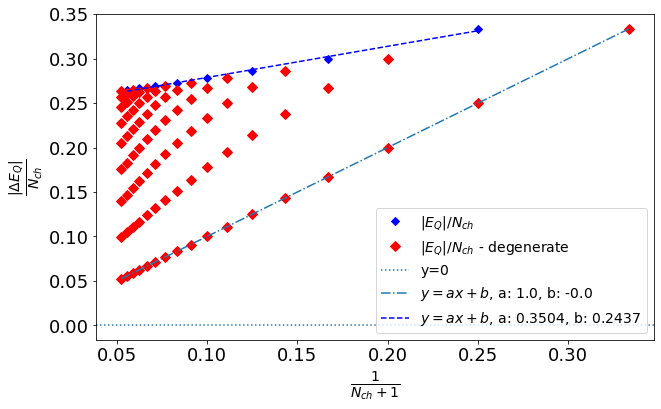
\includegraphics[scale=0.34]{plt/Quantum_Energy_per_channel}
\caption{This shows the variation of quantum energy per channel with $1/N$, where $N=N_{ch}+1$ is the total number of spins in the systems including the impurity spins. }
\label{fig:quantum_energy}
\end{figure}
\noindent In the stargraph model Hamiltonian there is a classical ising term ($S_d^zS^z$) and a quantum fluctuation term. Here we are interested in the energy expectation value arising from the quantum fluctuation part of the Hamiltonian (eq.\ref{eq:stargraph_hamiltonian}). We define ising enregy $E_{ising}$ and quantum energy $E_{Q}$ in the ground state $|\psi_g\rangle$ as,
\begin{eqnarray}
E_{ising} = |\langle \psi_g | \mathcal{H}^c_0 | \psi_g \rangle|, E_{Q} &=& |\langle \psi_g | \mathcal{H}^Q_0 | \psi_g \rangle|=|E_g|-|E_{ising}|~, \nonumber\\
&=& {\alpha S_d(S+1)}- |E_{ising}|.
\end{eqnarray}  
This quantum energy $E_Q$ is generated by the spin-flips between the impurity spin and the outer spin. Our goal here to understand the nature of this $E_Q$ as we go to the large $K$ limit, whether there are some remenant quantum fluctuation even in the thermodynamic limit. To answer that questio we intrduce another important parameter, quantum enrgy per channel, $e_Q=|E_Q|/K$ . We know in the gorund state $K=2S$ thus,
\begin{eqnarray}
e_Q &=& \frac{\alpha S_d(S+1)}{K} - \frac{|E_{ising}|}{K} ~,~\nonumber\\
%&=& \alpha\frac{(N_{ch}+2)}{4N_{ch}}-\frac{|E_{ising}|}{N_{ch}} ~,~ \nonumber\\
%&=& \alpha \bigg(\frac{1}{4} +\frac{1}{2N_{ch}} \bigg)-\frac{|E_{ising}|}{N_{ch}}~,~\nonumber\\
&=& \frac{\alpha S_d}{2} -\frac{1}{K} \bigg(|E_{ising}| -\alpha S_d  \bigg)~,~
\end{eqnarray}
Thus from the above equation of quantum energy per channel one can see that in the large channel limit 
\begin{eqnarray}
e_Q = \frac{\alpha S_d}{2}- \frac{|E_{ising}|}{K} < \frac{\alpha S_d}{2}~,~K\rightarrow \infty, 
\end{eqnarray}
As shown in the above Fig.\ref{fig:quantum_energy} for the case of $S_d=1/2$, for a particular channel $K$ the maximum quantum energy corresponds to the $|J^z|_{min}$ state and the minimum is related to the $|J^z|=J$ state. In the large channel limit one can see the quatnum energy associated with the $|J^z|=J$ vanishes showing the classical nature of this state where there is no quantum fluctuation present. Whereas, in the state $|J^z|_{min}$ there are finite non-zero quantum fluctuation present in it, showing the true quantum nature of this macroscpic singlet state as we have already discussed.



\subsection{Measure of quantum fluctuations}
\noindent Here we want to calculate various correlation functions in the ground state. We know that $J^z$ is a good quantum number, can take values $2J+1$ possible values. Here we are interested in calculating the quantum fluctuation present in the  ground state by measuring the expectation value of ${\mathcal{Q}}\equiv \langle \psi_g | (J^x)^2+(J^y)^2 |\psi_g\rangle$. We can see that ${\mathcal{Q}}= \langle \psi_g | J^2 - (J^z)^2 |\psi_g\rangle$. For a general $S_d$ impurity spin problem, $J=|K/2-S_d|$ in the ground state, thus $J^2=J(J+1)=(|K/2-S_d|)(|K/2-S_d|+1)$. We define a quantity $\Delta=(K/2-S_d)$, where $\Delta=0$ represents the exactly screened problem, $\Delta>0$ and $\Delta<0$ represents the overscreened and underscreened problem respectively. For the cases where $|\Delta|$ is integer $J^z_{min}=0$ and when $|\Delta|$ is half integer $J^z_{min}\pm 1/2$. Here we are intersted in calculating the maxmum quantum fluctuation present in the multi-channel zero mode ground state.
\begin{eqnarray}
\mathcal{Q}_{max}&=&   \langle \psi_g | J^2 - (J^z_{min})^2 |\psi_g\rangle \nonumber\\
&=&(|K/2-S_d|)(|K/2-S_d|+1)-1/4~,~~\textrm{$2|\Delta|$=odd}~~  \nonumber\\
&=&(|K/2-S_d|)(|K/2-S_d|+1) ~,~~\textrm{$2|\Delta|$=even}~~
\end{eqnarray}
Then maximum quantum fluctuation per channel is defined as $q_K=\sqrt{\mathcal{Q}_{max}}/K$. We find
\begin{eqnarray}
%q_K &=&  \sqrt{\frac{1}{4}-\frac{S_d}{K}+\frac{1}{2K}+\frac{S_d(S_d-1)}{K}}
q_K &=&  \frac{1}{K} \sqrt{|\Delta|(|\Delta|+1)}
%=\sqrt{\frac{1}{4}+\frac{1+2S_d^2-4S_d}{K}}
\end{eqnarray}
We can see that at large channel limit is, $\lim_{K\rightarrow \infty} q_K= 1/2$. Thus at large channel limit both the 
overscrened and underscreend ground states has same non-zero quantum fluctuation. Only for the exactly screened cases ($\Delta=0$) with unique ground state, this measure of quantum fluctuation $\mathcal{Q}_{max}$ vanishes. This shows the duality between overscreened and underscreened cases and it's distinction from the exactly screened cases.

%
%\begin{eqnarray}
%j_z^2&=&\frac{1}{N_{ch}}\langle \psi_g | J_z^2 | \psi_g \rangle~=\frac{1}{N_{ch}} \bigg[ J^2-(J_x^2+J_y^2) \bigg] ~,\nonumber\\
%%&=& \frac{1}{N_{ch}} \bigg[ (S^2-1/4)-(J_x^2+J_y^2) \bigg] \nonumber\\
%&=& \frac{1}{N_{ch}} \bigg[ \frac{(N_{ch}^2-1)}{4}-(J_x^2+J_y^2) \bigg]
%\end{eqnarray}
%
%\begin{eqnarray}
%\langle \psi_g | J_{z}^2 | \psi_g \rangle_{max} &=& \bigg(\frac{N_{ch}-1}{2}\bigg)^2~,\nonumber\\
%\langle \psi_g | J_{z}^2 | \psi_g \rangle_{min} = \bigg(\frac{N_{ch}-(N_{ch}-1)}{2}\bigg)^2&=&\frac{1}{4}~,~\textrm{for $N_{ch}$ even}.\nonumber\\
%&=& 0 ~,~\textrm{for $N_{ch}$ odd}.
%\end{eqnarray}
%Thus,
%\begin{eqnarray}
%\langle (J_x)^2+(J_y)^2 \rangle_{max}&=&\langle J^2 \rangle - \langle J_z^2 \rangle_{min} ~,\nonumber\\
%&=& \frac{N_{ch}^2-1}{4}-\frac{1}{4}=\frac{N_{ch}^2-2}{4}~, \textrm{for $N_{ch}$ even } \nonumber\\
%&=& \frac{N_{ch}^2-1}{4}~, \textrm{for $N_{ch}$ odd } \nonumber
%\end{eqnarray}
%Which shows, for single channel case $N_{ch}=1$, this quntum fluctuation expectation value vanishes, while for multi channel this takes non-zero values. Thus 
%\begin{eqnarray}
%\frac{1}{N_{ch}}\langle (J_x)^2+(J_y)^2 \rangle_{max}
%&=& \frac{N_{ch}}{4}-\frac{1}{2N_{ch}}  ~, \textrm{for $N_{ch}$ even } \nonumber\\
%&=& \frac{N_{ch}}{4}-\frac{1}{4N_{ch}}~, \textrm{for $N_{ch}$ odd } \nonumber
%\end{eqnarray}
%Thus in the large channel number limit $N_{ch}\gg 1$, one can see that 
%\begin{eqnarray}
%\frac{1}{N_{ch}}\langle (J_x)^2+(J_y)^2 \rangle_{max}
%\rightarrow \frac{N_{ch}}{4}~,~\textrm{for both even and odd $N_{ch}$}
%\end{eqnarray}
%\noindent $J_z$ can take values $\{-J,-J+1,\cdots,J-1,J\}$ in the ground state, where $J=S-1/2=(N_{ch}-1)/2$.
%
%



\subsection{Staggerred magnetization of the star graph}
\noindent  One can reqrite the Hamiltonian as $\alpha \vec{S}_d.\vec{S}=(\alpha/4) [( \vec{S}+\vec{S}_d)^2-( \vec{S}-\vec{S}_d)^2]$, this shows that $\vec{J}$ and the staggered magnetization $\vec{M}_s=\vec{S}-\vec{S}_d$ is both good quantum number for in this stargraph model. For single channel case $K=1$, ground state is an unique 2-spin singlet $|\psi_g\rangle =\frac{1}{\sqrt{2}} (|\uparrow\downarrow\rangle-|\downarrow\uparrow\rangle = |J=0,J_z=0\rangle$, which showns the prefect screening. Our goal here to capture the breakdown of the screening by calculating this staggerd magnetization for a multichannel problem. 
\begin{figure}
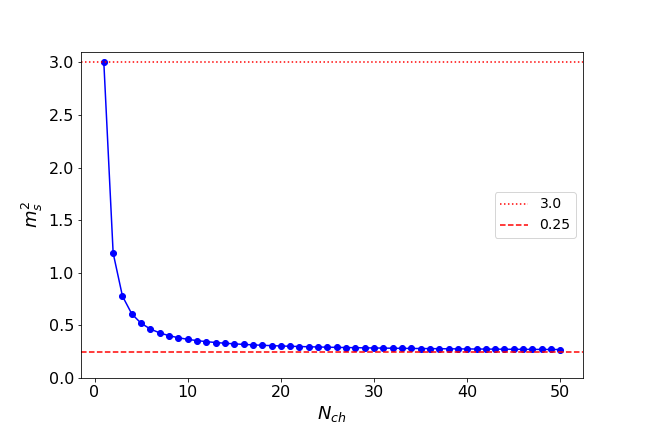
\includegraphics[scale=0.36]{plt/Staggered_mag_50.png}
\caption{This shows how the staggered magnetization changes with the number of channels $N_{ch}$.}
\label{fig:st_mag}
\end{figure}
%
%
%For the single channel case both the $\vec{S}_d$ and $\vec{S}$ are spin-1/2 object and the total spin is defined as $\vec{J}=\vec{S}_d+\vec{S}$. Here $\vec{S}$ is the total outer spin.
%
%\begin{eqnarray}
%M_s^2 = \langle \psi_g | (\vec{S}_d - \vec{S})^2 |\psi_g\rangle &=& \langle \psi_g | 2(\vec{S}_d^2 + \vec{S}^2)-\vec{J}^2 |\psi_g\rangle \nonumber\\
%&=& 2 \langle \psi_g | \vec{S}_d^2 +\vec{S}^2 |\psi_g\rangle \nonumber\\
%&=& 3
%\end{eqnarray}
For a general $K$ cahnnel we find that 
\begin{eqnarray}
M_s^2 &=& \langle \psi_g | (\vec{S}_d - \vec{S})^2 |\psi_g\rangle = \langle \psi_g | 2(\vec{S}_d^2 + \vec{S}^2)-\vec{J}^2 |\psi_g\rangle \nonumber\\
%&=&    2\bigg(S_d(S_d+1)+ \frac{K(K+2)}{4}\bigg)- \frac{(K+1)(K-1)}{4}   \nonumber\\
%&=& 2S_d(S_d+1) + \frac{1}{2}(K^2+2K) - \frac{1}{4}(K^2-1)\\
&=& 2S_d(S_d+1) +\frac{K^2}{4} + K +\frac{1}{4}
%%%%&=& \frac{N_{ch}^2}{4}+N_{ch}+\frac{7}{4}
\end{eqnarray}


\noindent Thus, staggered magnetization squared per channel,
\begin{eqnarray}
m_s^2=\frac{M_s^2}{K^2}= \frac{2S_d(S_d+1)}{K^2}+\frac{1}{4}+\frac{1}{K}+\frac{1}{4K^2}
%=\frac{1}{4}+\frac{1}{N_{ch}}+\frac{7}{4N_{ch}^2} \xrightarrow[]{N_{ch}\gg 1} \frac{1}{4}+\frac{1}{N_{ch}}~,
\end{eqnarray}
Which shows, in the large channel limit this staggered magnetization , $m^2_s\Rightarrow 1/4.$ for any finite $S_d$.
Using the $SU(2)$ property of our problem, we can define $m_s$ for each spatial direction, in 3D there are three independent spatial direction.
\begin{eqnarray}
\langle(m_s^x)^2\rangle=\langle(m_s^y)^2\rangle=\langle(m_s^z)^2\rangle=\frac{1}{3}m_s^2~,~~   
\end{eqnarray}
Just to recall, for the single channel case $\langle (m_s^z)^2 \rangle =1$ showing the perfect screening, on the otherhand in the large channel limit this becomes $\langle (m_s^z)^2 \rangle =1/12$ showing the breakdown of the screening. For the $S_d=1/2$ case we have shown how this staggered magnetization perchannel decreases in the multichannel case in the Fig.\ref{fig:st_mag}. This clearly shown that this staggerd magnetization is maximum.


%\begin{eqnarray}
%\frac{\vec{J}^2}{N_{ch}^2}&=&\frac{(\vec{S}_d+\vec{S})^2}{N_{ch}^2}= \frac{N^2_{ch}-1}{4N^2_{ch}} \xrightarrow[]{N_{ch}\gg 1} \frac{1}{4}~. \nonumber 
%\end{eqnarray}
%
%
%To begin with we first recall that for single channel case $M_s^2=3$.
%
%We define $m_Q^2=m_s^2-1/4$ which in the the large $N_{ch}$ limit becomes $1/N_{ch}$ and eventually vanishes in the $N_{ch}\rightarrow \infty$ limit. 
%
%
%\noindent Thus to summarize,
%\begin{enumerate}
%\item In the single channel problem, $\langle (m_s^z)^2 \rangle=1$. 
%\item In the multi-channel case,  
%$\langle (m_s^z)^2 \rangle=\frac{1}{3N_{ch}}+\frac{1}{12}+\frac{7}{12N_{ch}^2} \xrightarrow[]{N_{ch}\gg 1} \frac{1}{12}+\frac{1}{3N_{ch}}\rightarrow \frac{1}{12}$. 
%This show partial screening.
%\end{enumerate}



%\subsubsection{Degree of compensation: a measure of the frustration}
%One can quantify the amount of screening of the local moment at the impurity site by defining a degree of compensation \(\kappa\). Such a quantity also measures the inherent singlet frustration in the problem: the higher the degree of compensation, the better the spin can be screened into a singlet and lower is the frustration. It is given by the antiferromagnetic correlation existing between the impurity spin and conduction electron channels:
%\begin{equation}\begin{aligned}
%	\Gamma \equiv - \left< \vec{S_d}\cdot \vec{s}_\text{tot}\right>
%\end{aligned}\end{equation}
%where \(\vec s_\text{tot} = \sum_l \vec s_l\). The expectation value is calculated in the ground state. Since the inner product is simply the ground state energy of a spin-\(S\) impurity \(K-\)channel MCK model in units of the exchange coupling \(J\), we have
%\begin{equation}\begin{aligned}
%	\Gamma = \frac{1}{2} \left[ l_\text{imp}^2 + l_c^2 - g^S_K\left( g^S_K - 1 \right)\right]
%\end{aligned}\end{equation}
%\(l_\text{imp}^2 = S(S+1)\) is the length-squared of the impurity spin. Similarly, \(l_c^2 = \frac{K}{2}\left(\frac{K}{2} + 1\right) \) is the length-squared of the total conduction bath spin. \(g^S_K = |\frac{K}{2} - S| + 1\) is the ground state degeneracy. We will explore the three regimes of screening by defining \(K = K_0 + \delta, S = \frac{K_0}{2} - \delta\). \(\delta=0\) represents the exactly-screened case of \(K = 2S = K_0\). Non-zero \(\delta\) represents either over- or under-screening. In terms of \(K_0\) and \(\delta\), the degree of compensation becomes
%\begin{equation}\begin{aligned}
%	\label{gamma}
%	\Gamma = \frac{1}{4}\left[\left( K_0 + 1 \right) ^2 - \left(|\delta| + 1 \right) ^2\right] 
%\end{aligned}\end{equation}
%\textit{For a given \(K_0\), the degree of compensation is maximised for exact screening \(\delta=0\), and is reduced for \(\delta \neq 0\). This shows the inability of the system to form a unique singlet ground state and reveals the quantum-mechanical frustration inherent in the zero mode Hamiltonian and therefore in the entire problem.} The degree of compensation is symmetric under the Hamiltonian transformation \(\delta \to -\delta\), and this represents a duality transformation between over-screened and under-screened MCK models. This topic will be discussed in more detail later.
%\begin{figure}[htpb]
%	\centering
%	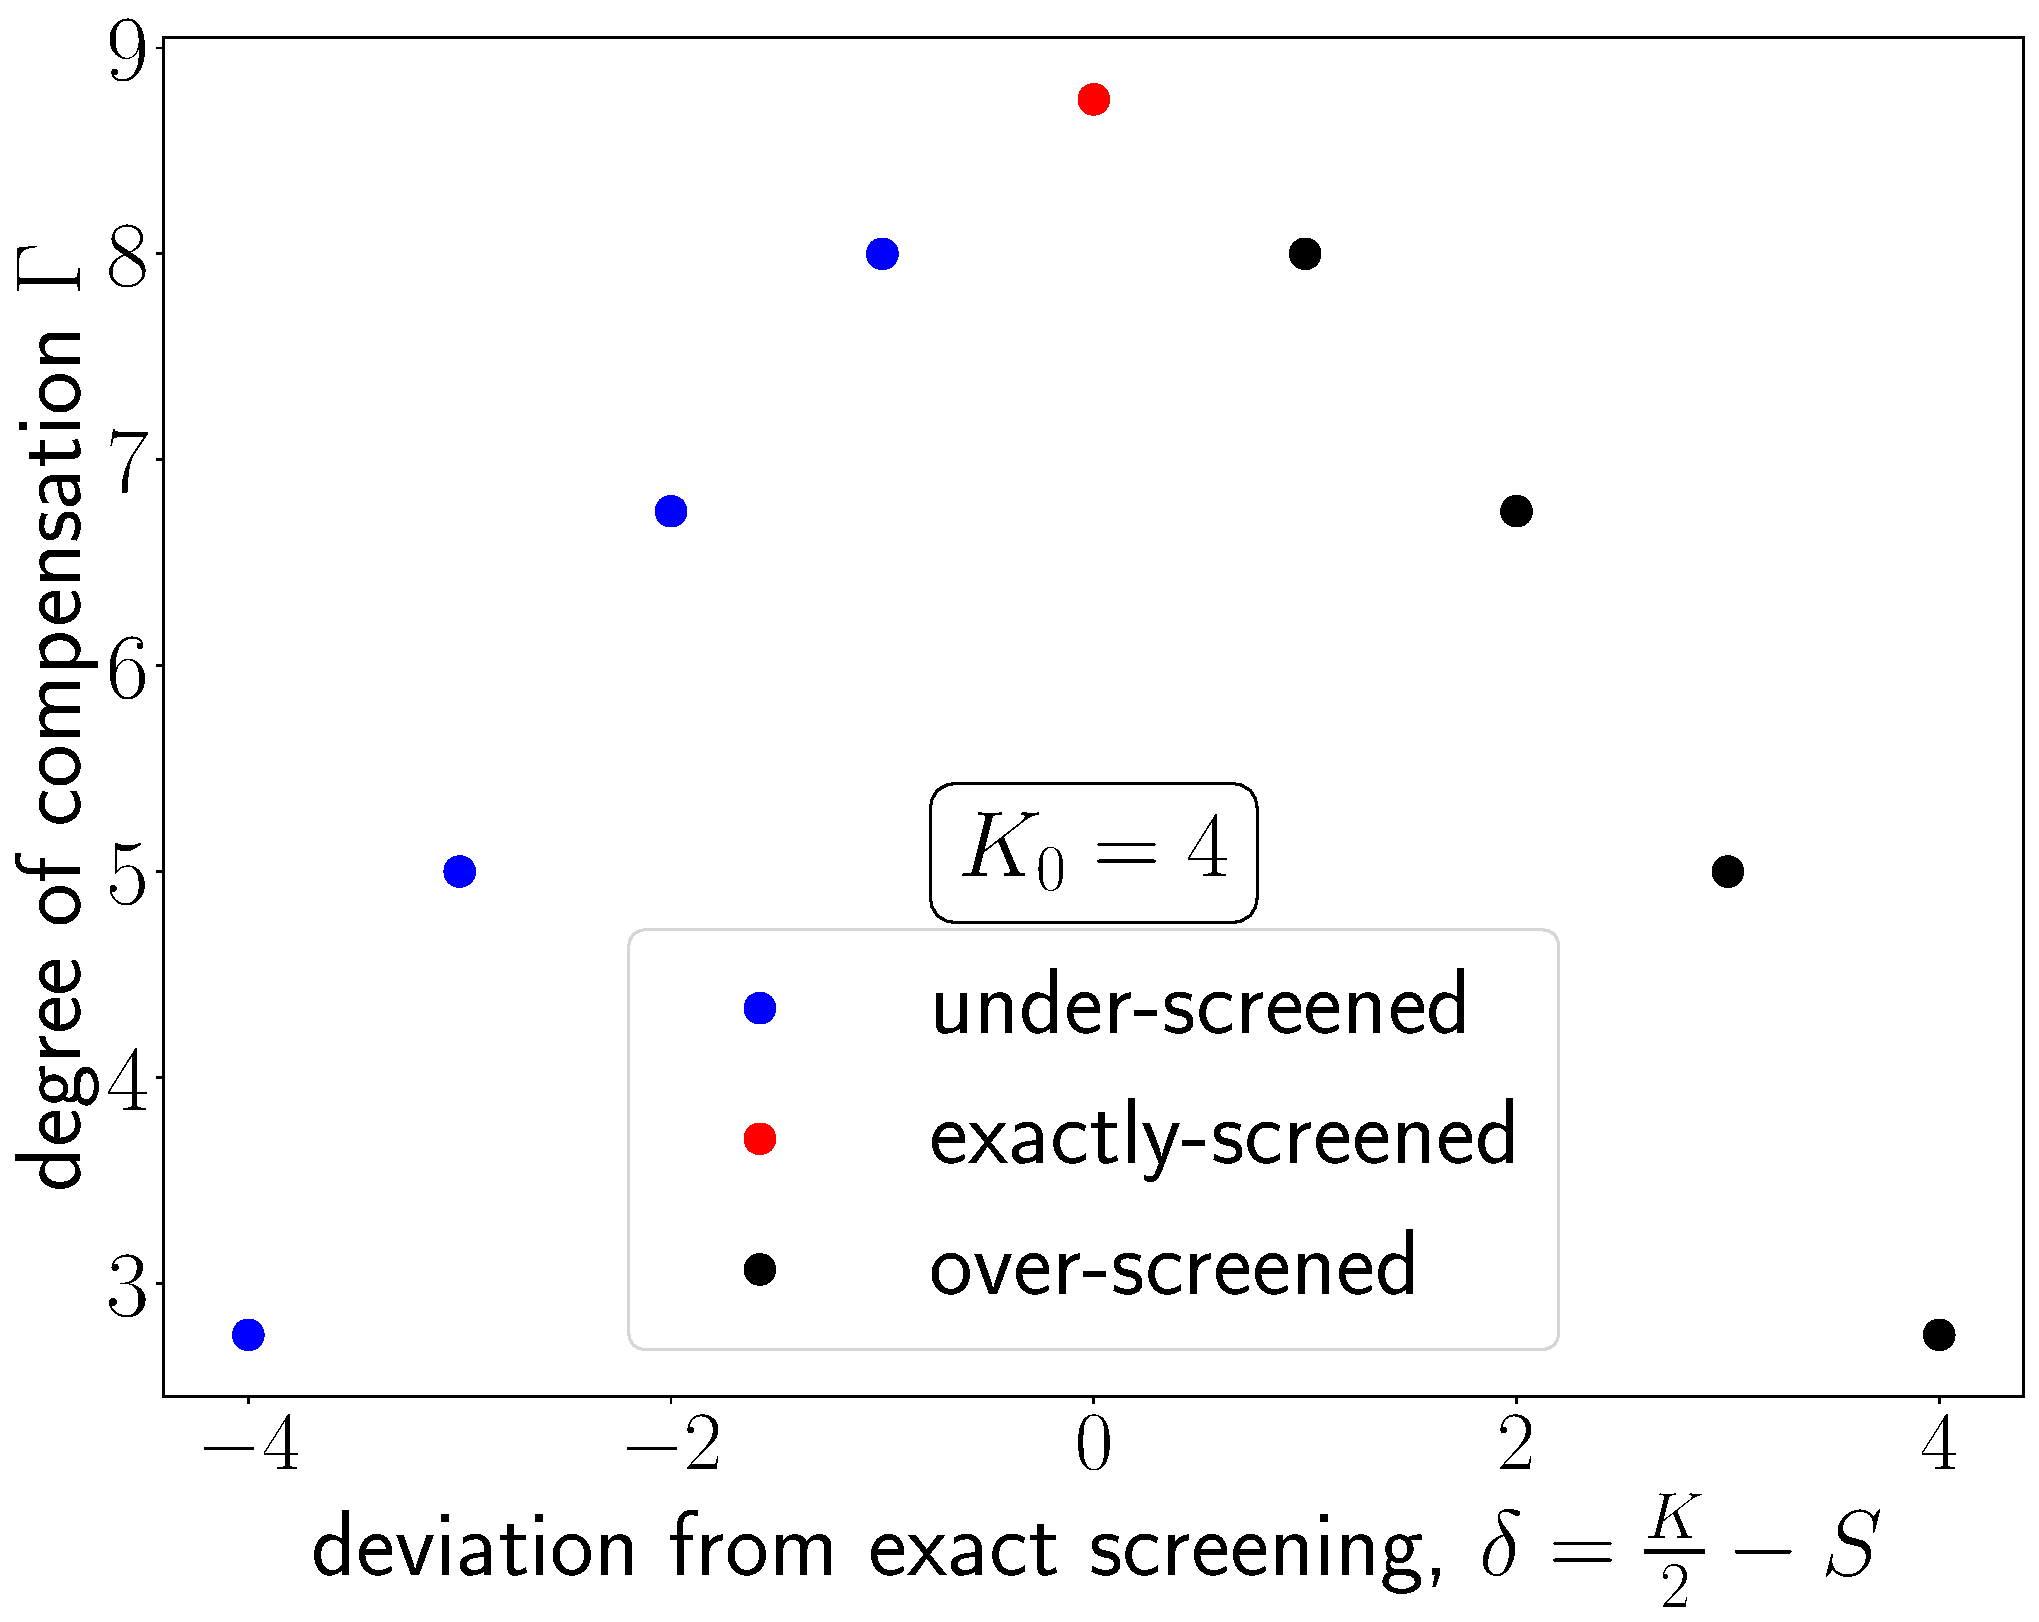
\includegraphics[width=0.45\textwidth]{plt/deg_of_comp.pdf}
%	\caption{Variation of the degree of compensation as we tune the system from under-screening to over-screening. The maximum spin compensation occurs at exact-screening \(\delta=0\).}
%\end{figure}

%\subsection{Measures of entanglement}

%\subsection{Twist operators and Gauge theories}

\subsection{Thermodynamic quantitites}
%\subsubsection{Impurity magnetization and susceptibility: Quantum criticality of overscreened MCK model}
%The channel isotropic MCK model is critical; any perturbation away from the perfectly symmetric model in terms of anisotropy is relevant, as shown in section \ref{anisotropic_rg}~\cite{vojta_2006,andrew_bulla_2011,pang_cox_1991}. This critical nature leads to several signatures that can be obtained directly from the star graph. These signatures include a discontinuity in the impurity magnetization at zero temperature in the limit of the external field going to zero, and a diverging susceptibility as temperature goes to zero.
%
%We insert a magnetic field that acts only on the impurity and then diagonalize the Hamiltonian.
%\begin{align}
%	\label{stargraph_field_hamiltonian}
%	H(h) = J^* \vec{S_d}\cdot\vec{s}_\text{tot} + h S_d^z
%\end{align}
%The Hamiltonian commutes with \(s_\text{tot}\), so it is already block-diagonal in terms of the eigenvalues \(M\) of \(s_\text{tot}\). \(M\) takes values in the range \(\left[M_\text{min}, M_\text{max}\right]\), where \(M_\text{max} = K/2\) for a \(K-\)channel Kondo model, and \(M_\text{min} = 0\)  if \(K\) is even, otherwise \(\frac{1}{2}\). Within each block, the Hamiltonian splits into independent \(2\times 2\) blocks characterized by eigenvalues of the total spin operator \(J^z = S_d^z + s^z_\text{tot}\). Defining \(\alpha = \frac{1}{2}\left(Jm + h\right) + \frac{J}{4}\) and \(x^M_m = M(M+1) - m(m+1)\), the partition function can be written as
%\begin{align}
%	Z(h) =\sum_{M=M_\text{min}}^{M_\text{max}}r^K_M\left[\sum_{m=-M, \atop{m\in \mathbb{Z}}}^{M-1}2e^{\beta \frac{J}{4}}\cosh \beta\sqrt{J^2x^M_m/4 + \alpha^2} \right.\nonumber\\
%\left.+ 2e^{-\beta JM/2}\cosh \beta h/2\right]
%\end{align}
%Here, \(\beta = \frac{1}{k_B T}\), \(M\) sums over the eigenvalues of \(s_\text{tot}\) while \(m\) sums over \(J^z - \frac{1}{2}\) and the additional degeneracy factor \(r^K_M\) arises from the possibility that there are multiple subspaces defined by \(s_\text{tot}=M\). This multiplicity is given by
%\begin{align}
%	\label{extra_degen}
%	r^K_M = {}^{K-1}C_{K/2 - M}
%\end{align}
%
%To calculate the impurity magnetic susceptibility, we will use the expression
%\begin{align}
%	\chi = \frac{1}{\beta}\lim_{h \to 0}\left[\frac{Z(h)^{\prime\prime}}{Z(h)} - \left(\frac{Z(h)^{\prime}}{Z(h)}\right)^2 \right] 
%\end{align}
%where the \(\prime\) indicates derivative with respect to \(h\). For brevity, we define \(\theta_M = \beta J (M+\frac{1}{2})/2\) and \(\Sigma_M = \sum_{m=-M, \atop{m\in \mathbb{Z}}}^{M-1}(m+\frac{1}{2})^2\). The derivatives are
%\begin{align}
%	\lim_{h \to 0}Z(h) &= \sum_{M=M_\text{min}}^{M_\text{max}}r^K_M\left[4Me^{\beta \frac{J}{4}}\cosh \theta_M + 2e^{-\beta JM/2}\right]\\
%	\lim_{h \to 0}\frac{\:\mathrm{d}Z(h)}{\:\mathrm{d}h} &=  0\\
%	\lim_{h \to 0}\frac{\:\mathrm{d}^2Z(h)}{\:\mathrm{d}h^2} &= \frac{\beta^2}{2}\sum_{M=M_\text{min}}^{M_\text{max}}r^K_M\left[\frac{e^{\beta \frac{J}{4}}}{\theta_M}\left(2M\sinh \theta_M + \right.\right.\nonumber\\
%								 &\left.\left.\frac{\beta^2 J^2}{4}\left[\frac{\cosh\theta_M}{\theta_M} - \frac{\sinh \theta_M}{\theta_M^2}\right]\Sigma_M\right)+ e^{-\beta JM/2}\right]
%\end{align}
%At low temperature \(\beta \to \infty\), only the highest value \(M_\text{max}\) will survive:
%\begin{align}
%	Z &\to 2 r^K_{M_\text{max}} M_\text{max} e^{\beta \frac{J}{2}(M_\text{max} + 1)}\\
%	Z^{\prime \prime} &\to r^K_{M_\text{max}}\left(\frac{\beta }{2(M_\text{max} + \frac{1}{2})}\right)^2 e^{\beta \frac{J}{2}(M_\text{max} + 1)}\Sigma_{M_\text{max}}\\
%	\chi &\to \frac{\beta\Sigma_\text{max}}{2M_\text{max}\left(2M_\text{max}+1\right)^2} = \frac{\beta(K-1)}{12(K+1)} \sim \frac{1}{T}
%\end{align}
%
%\textit{This non-analyticity in a response function is a signature of the critical nature of the Hamiltonian. This is in contrast to the behaviour in the non-critical exactly-screened fixed point where the ground state is unique.} There, the susceptibility becomes constant at low temperatures: \(\chi(T\to 0) = \frac{W}{4 T_K}\), \(T_K\) being the single-channel Kondo temperature and \(W\) the Wilson number \cite{wilson1975renormalization,nozieres1974fermi,bullaNRGreview,kondo_urg}. We have checked the case of general spin-\(S\) impurity numerically, and the general conclusion is that all exactly-screened models show a constant impurity susceptibility at \(T \to 0\), while the over-screened and under-screened cases show a diverging impurity susceptibility in the same limit. 
%
%Another non-analyticity arises when we consider the impurity free energy and the magnetization. The thermal free energy is given by
%\begin{equation}\begin{aligned}
%	F(h) = -\frac{1}{\beta}\ln Z(h) = -\frac{1}{\beta}\ln\sum_{E_n}e^{-\beta E_n}
%\end{aligned}\end{equation}
%At \(T \to 0\), only the most negative energy \(E_\text{min}\) survives. Assuming a non-degenerate ground state for \(h \neq 0\), the zero temperature free energy becomes
%\begin{equation}\begin{aligned}
%	F(h\neq 0, T\to 0) = -\frac{1}{\beta}\ln e^{-\beta E_\text{min}} = E_\text{min}
%\end{aligned}\end{equation}
%In the star graph Hamiltonian with \(K-\)channels and in the presence of a field on the impurity (eq.~\ref{stargraph_field_hamiltonian}), the ground state energy will be one of the negative eigenvalues:
%\begin{equation}\begin{aligned}
%	\lambda^{M,h}_{m, -} = - \frac{J}{4} - \frac{1}{2}\sqrt{J^2(M+1/2)^2 + h^2 + 2hJ(m+1/2)}
%\end{aligned}\end{equation}
%The minimum eigenvalue is obtained by maximizing \(h(m+1/2)\). For \(h>0\), the ground state is renormalised for the most positive value of \(m\), which is \(M-1\). On the other hand, for \(h<0\), it occurs for \(m=-M\), because that is the most negative value it can take. Among all the values of \(M\), the global ground state is at the largest value of \(M\), \(K/2\). Therefore, the minimal energy eigenvalue is
%\begin{equation}\begin{aligned}
%	E_\text{min} = - \frac{J}{4} - \frac{1}{2}\sqrt{J^2(K+1)^2/4 + h^2 + |h|J(K-1)}
%\end{aligned}\end{equation}
%The first derivative of the free energy with respect to the field gives
%\begin{equation}\begin{aligned}
%	F^\prime(h\neq 0, T\to 0) =- \frac{2h + J(K-1)\text{sign}(h)}{4\sqrt{\frac{J^2}{4}(K+1)^2 + h^2 + |h|J(K-1)}}
%\end{aligned}\end{equation}
%There we used the result that the derivative of \(|x|\) is \(\text{sign}(x)\). If we now take \(h\) to zero from both directions, we get the magnetization of the impurity
%\begin{equation}\begin{aligned}
%	m = F^\prime(h \to 0^\pm, T\to 0) = \mp \frac{1}{2}\frac{(K-1)}{(K+1)}
%\end{aligned}\end{equation}
%\begin{figure}[!htpb]
%	\centering
%	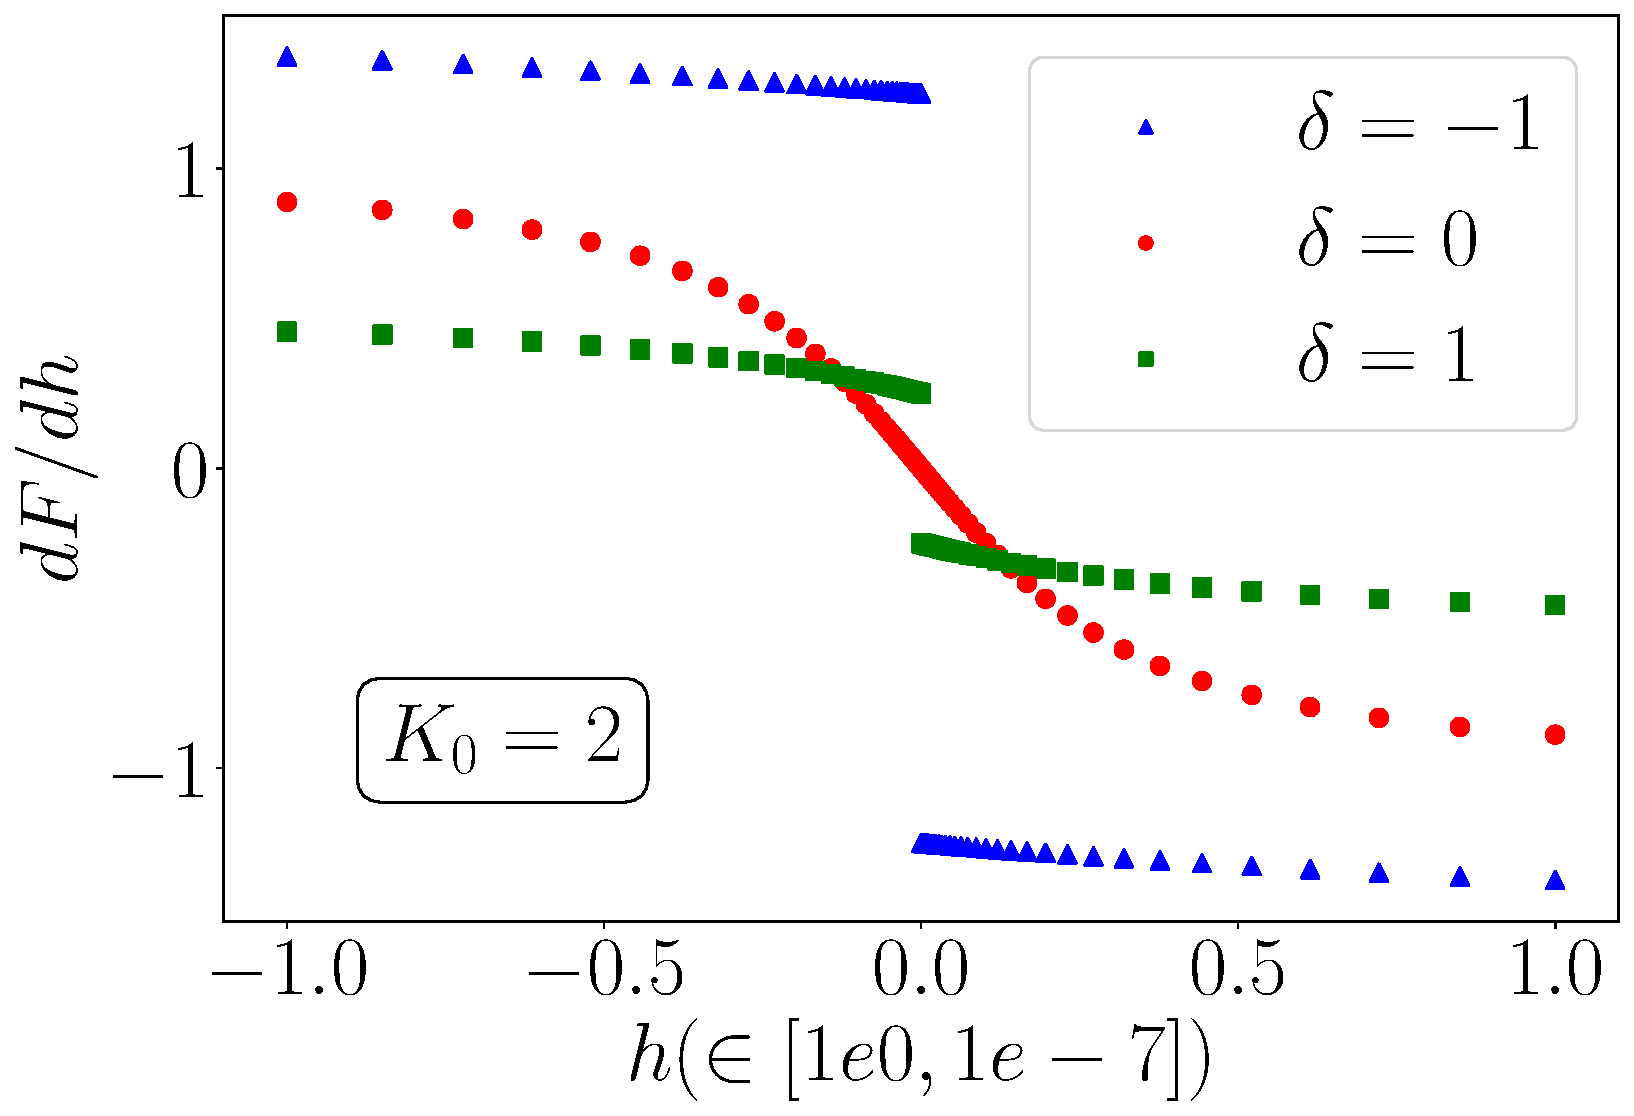
\includegraphics[width=0.45\textwidth]{plt/disc_mag_imp_gen.pdf}
%	\caption{Behaviour of the impurity magnetization for three values of \(\left(K, 2S\right) = \left(2, 4\right), \left( 3,3 \right), \left(4, 2\right)  \). Only the case of \(K=2S=3 \left(\delta=0\right)\) is analytic near zero. The non-analyticity of the other cases arises because of the frustration brought about by the degeneracy of the star graph ground state.}
%	\label{mag_crit}
%\end{figure}
%
%The magnetization is therefore discontinuous as \(h\to 0\); it goes to different values depending on the direction in which we take the limit. The non-analyticity for \(K>1\) occurs because there is at least one pair of ground state with non-zero parity \(\pi^z\) and magnetic field is able to flip one ground state into the state of opposite parity. This available space for scattering is simply the frustration that we discussed earlier. This argument, along with the diverging susceptibility for the over- and under-screened cases, makes it clear that \textit{the non-analyticity and hence the critical nature of the fixed point arise because of the ground state degeneracy, and is therefore a feature of all over-screened and under-screened  models}. Indeed, we have checked numerically (see fig.~\ref{mag_crit}) that the non-analyticity exists for \(\delta \neq 0\), where \(\delta = \frac{K}{2} - S\) is the deviation from exact screening. For \(\delta=0\), the ground state is unique and un-frustrated, so the external magnetic field has no parity-inverted pair to flip across.

\subsubsection{Impurity magnetization in terms of parity operators}
Just like the complete string operator \(\pi^z\), the modified string operator \(\sigma_d^z \pi^z\) is also a Wilson loop operator that wraps around only the outer nodes of the star graph:
\begin{equation}\begin{aligned}
	\pi^z_c \equiv \sigma_d^z \pi^z = \exp\left[i \frac{\pi}{2} \left(\sum_{l=1}^K \sigma^z_l - K\right)\right] 
\end{aligned}\end{equation}
The expectation value of the impurity magnetization along a particular direction and in specific ground states can be related to the 't Hooft operator defined under eq.~\ref{w_loop}. We will work in the state comprised of two adjacent eigenstates of \(J^z\):
\begin{equation}\begin{aligned}
	\ket{g^\theta_{J^z}} \equiv \frac{1}{\sqrt 2}\left( \ket{J^z} + e^{i\theta}\ket{J^z+1}\right), && J^z < \frac{1}{2}\left( K-1 \right)
\end{aligned}\end{equation}
The expectation value of the impurity magnetization operator \(\sigma_d^x\) can be expressed as
\begin{equation}\begin{aligned}
	\left<\sigma_d^x\right> \equiv \langle g^\theta_{J^z} \vert \sigma_d^x \vert g^\theta_{J^z}\rangle = - \langle J^z + 1 \vert \pi^x_c \vert -J^z \rangle + \text{h.c.}
\end{aligned}\end{equation}
This expression relates the observable impurity magnetization to the topological 't Hooft operator \cite{Maric2020}. Evaluating the matrix elements gives
\begin{equation}\begin{aligned}
	\label{sigmax}
	\left<\sigma_d^x\right> = - \frac{\sqrt{K^2 - (2J^z + 1)^2}}{2(1+K)}\cos \theta
\end{aligned}\end{equation}
Performing a similar calculation reveals that the impurity magnetizations along \(y\) and \(z\) in the same state are given by
\begin{equation}\begin{aligned}
	\label{sigmayz}
	\left<\sigma_d^y\right> = - \frac{\sqrt{K^2 - (2J^z + 1)^2}}{2(1+K)}\sin \theta, &&\left<\sigma_d^z\right> = - \frac{2J^z + 1}{(1+K)}
\end{aligned}\end{equation}
Combining eqs.~\ref{sigmax} and \ref{sigmayz}, we find
\begin{equation}\begin{aligned}
	\cos^2\theta\left(\left<\sigma^x_d\right>\right)^2 + \sin^2\theta\left(\left<\sigma^y_d\right>\right)^2 + \frac{1}{4}\left(\left<\sigma^z_d\right>\right)^2 = \frac{1}{4}\left(\frac{K}{1+K}\right)^2
\end{aligned}\end{equation}
\textit{This relation constrains the values of the magnetization along all the directions: the \(x\) and \(y\) magnetization values have already been shown to be related to the `t Hooft operators \(\pi^x\) and \(\pi^y\) and the magnetization along \(z\) is therefore constrained in terms of the `t Hooft operators and the quantized function on the right-hand side (the function is quantized because \(K\) can only take integer values).}


%\subsubsection{Plots}
%
%\noindent Here we want to calculate the field suseptibility of the stargraph. For that we need the entire spectrum of the stargraph Hamiltonian in the presence of field. There are two ways one can capture the suseptibility of the stargraph, first, by putting a small field to the central impurity and the other way is put a uniform field on all the outer spins and capture the suseptibility.
%
%\textit{Impurity-field susceptibility :} Now we add small magnetic field to the impurity spin and calculte the suseptibility as a function of temperatur for different channel cases.
%\begin{figure}[!h]
%\centering
%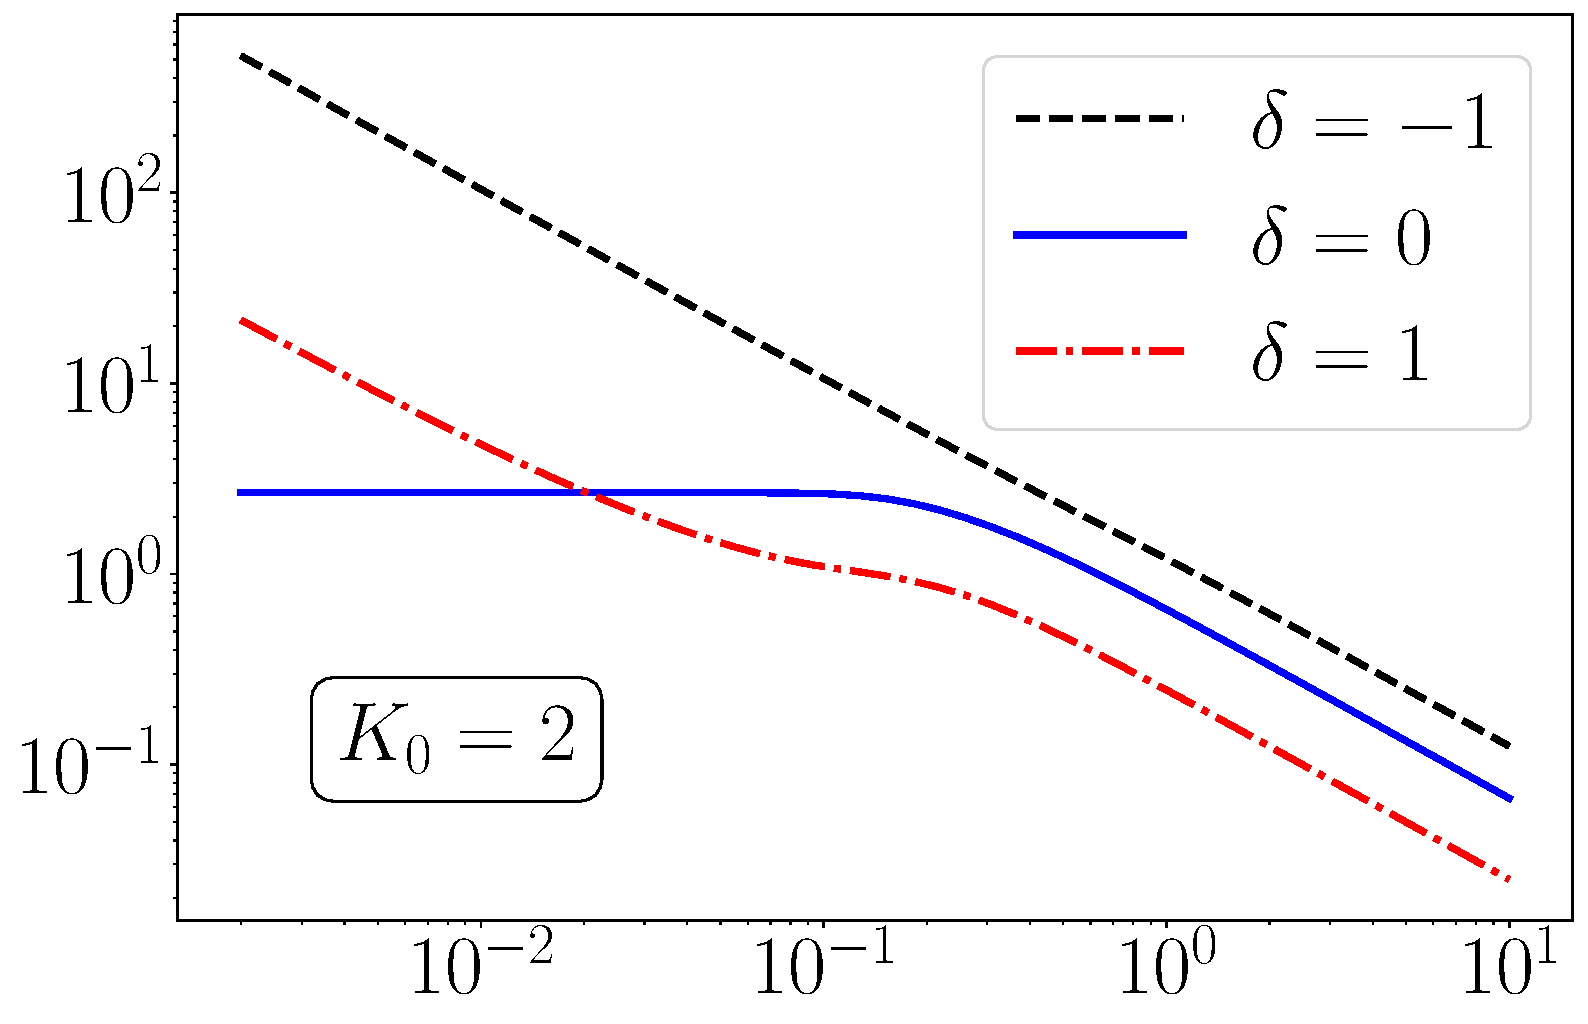
\includegraphics[scale=0.36]{plt/Central_Field_Chi_Powerlaw_}
%\caption{Impurity susseptibility vs temperature.}
%\label{fig:suseptibility_impurity}
%\end{figure}
%As shown in the Figure.\ref{fig:suseptibility_impurity} above, for all $K>2$ case we can see that, at low temperature the suseptibility follows power law as afunction of temperature. 
%\begin{eqnarray}
%\chi_{imp}(T) \sim T^{-1} ~,~ \chi_{outer} \sim T^{-1}
%\end{eqnarray}
%The exponent for all the channels $K>2$ is $-1$. This shows the presence of an universality class. The powerlaw shows the critical nature of the system.
%
%\textit{Outer-field suseptibility: } Similar study can be done by putting an uniform field on all outer spins and calculating the suseptibility. Here also for all channles $K>2$ the exponent is $-1$ and supports the existance of universality and criticality.
%\begin{figure}[!h]
%\centering
%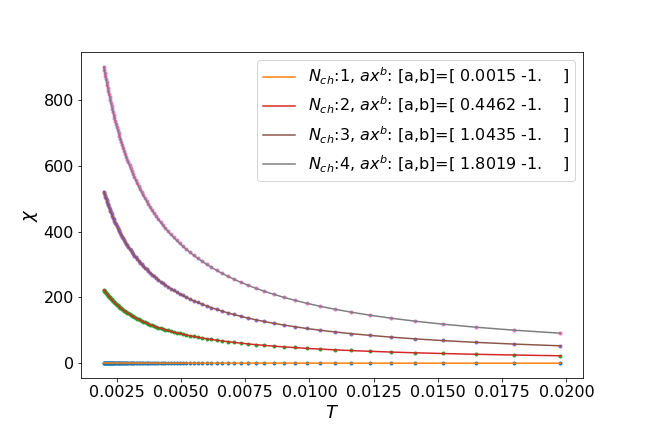
\includegraphics[scale=0.36]{plt/Outer_Field_Chi_Powerlaw_}
%\caption{Outer susseptibility vs temperature.}
%\label{fig:suseptibility_outer}
%\end{figure}
%This susceptibility clearly shown the breakdown of screening in the multichannel cases with degenerate ground states in constrast to the single channel suseptibility which saturates at a finite value at low temperature.


\subsubsection{Thermal entropy}
\noindent Thermal entropy is defined as $S=-(\frac{\partial \mathcal{F}}{\partial T})_H$, where $H$ represents a constant magnetic field. In ourcase we will be interested in the zero field case. 
\begin{eqnarray}
\mathcal{F}&=& -k_B T\log Z \nonumber\\
S &=& -(\frac{\partial \mathcal{F}}{\partial T}) = -k_B \log Z -k_B T \frac{1}{Z} \frac{dZ}{dT}
\end{eqnarray}
%Now 
%\begin{eqnarray}
%Z =\sum_\epsilon  d(\epsilon)e^{-\beta \epsilon} ~~\Rightarrow ~~  \frac{dZ}{dT} &=& \sum_\epsilon d(\epsilon) e^{-\beta \epsilon}  (-\epsilon) \frac{d\beta}{dT} \nonumber\\
%&=& \sum_\epsilon d(\epsilon) e^{-\beta \epsilon}   \frac{ \epsilon}{k_B T^2} =k_B\sum_\epsilon \epsilon d(\epsilon) e^{-\beta \epsilon} \beta^2   
%\end{eqnarray}
Thus we get
\begin{eqnarray}
S &=& -k_B \log \sum_{\epsilon} d(\epsilon) e^{-\beta \epsilon}  -\frac{1}{\beta} \frac{k_B\sum_\epsilon \epsilon d(\epsilon) e^{-\beta \epsilon} \beta^2   }{\sum_\epsilon  d(\epsilon)e^{-\beta \epsilon}} \nonumber\\
\lim_{\beta\rightarrow \infty} S &=& -k_B \log_2 d(\epsilon_{G})~,~~\lim_{\beta\rightarrow 0} S = -k_B \log \sum_\epsilon d(\epsilon)  \nonumber
\end{eqnarray}
\begin{figure}
\centering
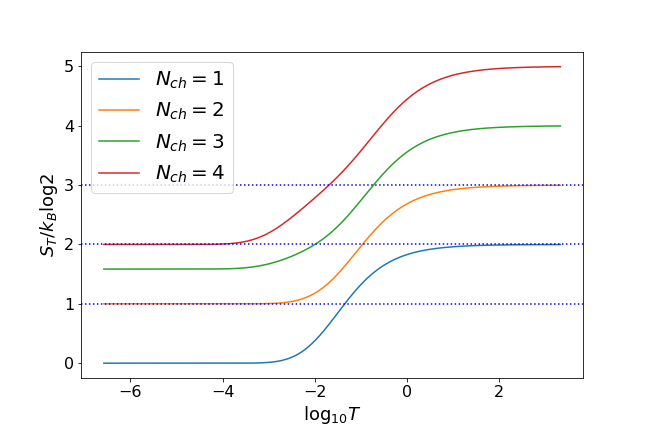
\includegraphics[scale=0.36]{plt/ThermalEntanglementVS_LogTemperature_}
\caption{This shows the variation of thermal entropy with the temperature.}
\label{fig:thermal_entropy}
\end{figure}
Thus at the extreme temperature it is easy to calculate the termal entropy, but it is difficult to visualize for any intermediate temperatures. Thus we plot the thermal entropy (unit $\log 2$) for different tempertures and for different channels in Fig.\ref{fig:thermal_entropy}. This shows at the extreme temperature the termal entropy saturates and at the intermediate temperature it changes from one to the other like a soliton like solution. At low temperature the thermal enttropy in the unit of $\log 2$ is not always quanlized but at high temperature it is. To understad this let's say at low temperature $S_T/k_B\log T=\Omega=\log_2 d(\epsilon_{G})$. Here $d(\epsilon_{G})$ is always integer and equal to the channel number $K$. Thus 
\begin{eqnarray}
d(\epsilon_{G}) &=& 2^{\Omega}=K
\end{eqnarray}
From our study we can see that for some channel number we get $S_T/k_B\log T$ tobe integer. One can easily see that those $K=2^n$ channel cases, $n$ is an integer will have integer thermal entropy. Thus between $m$ and $m+1$ integer thermal entropy plateau there will be $(2^m-1)$ number of fractional thermal entropy plateau, which is always odd.

\par Note, The above results for the high temperature holds for spin-1/2 impurity case, which slightly diffes for the case with general $S_d$ impurity spin, though the low temperature behavior only depends on the ground state degeneracy ($d_{\epsilon_G}=(K+1)-2S_d$) irrespective of the value of $S_d$. At high temperature the entanglement entropy depends on $\sum_{\epsilon} d(\epsilon)$, which is the dimension of the Hilbert space, $\sum_{\epsilon} d(\epsilon)=2^K\times (2S_d+1)$. Thus entanglemen entropy at high temperature for a general $S_d$ impurity spin is
\begin{eqnarray}
\lim_{\beta\rightarrow 0} S &=& -k_B \log \sum_{\epsilon} d(\epsilon)= -k_b \log [2^K (2S_d+1)]~,~~~
\end{eqnarray}
One can confirm that for $S_d=1/2$, $\lim_{\beta\rightarrow 0} S=-k_B(K+1)$. Thus only for those $S_d$ values when $2S_d+1=2^Q$, we get $-k_b \log [2^K (2S_d+1)]=-k_b (K+Q)$. Which shows that only some of the half integer impurity problems will have integer entanglement entropy at high temperature limit.


%\subsection{Gauge Theory and topology}
%\noindent  We can define two operators, for convenience let's call translation and twist operator respectively, $\hat{T}$ and $\hat{O}$ defined as 
%\begin{eqnarray}
%\hat{T} &=& e^{i\frac{2\pi}{K} \hat{\Sigma}} ~,~\hat{O} = e^{i\hat{\phi}}~,~~\hat{\Sigma}=[\hat{J}^z-(K-1)/2]
%\end{eqnarray}
%One can see that the generators of these above operators commutes with the Hamiltoninan, $[H,J^x]=[H,J^z]=[H,J^z]=0$. In the large channel limit we can do semiclaassical approximation. As $J^x$ and $J^y$ both commutes with the Hamiltonian $H$ then $[H,J^y{(J^{x})}^{-1}]=0$, and any non-singular function of these operators must also commute with the Hamiltonian, thus we can say that
%\begin{eqnarray}
%\hat{\phi}=\tan^{-1}(\hat{J}^y(\hat{J}^x)^{-1})
%\end{eqnarray}
%Then we get $[\hat{\phi},\hat{H}]=0$. We can label the ground states by the eigen values of the translation operator $\hat{T}$. We can also use the ground states labeled by the eigenvalues of $J^z$ ($M$, say). Then the ground states are 
%\begin{eqnarray}
%|M_1\rangle,|M_2\rangle,|M_2\rangle,\cdots ,|M_K\rangle
%\end{eqnarray}
%Then the operations of the translation operators on this states are give below.
%\begin{eqnarray}
%\hat{T}|M_i\rangle &=& e^{i\frac{2\pi}{K} [M_i-(K-1)/2]} |M_i\rangle = e^{i2\pi\frac{p_i}{K} } |M_i\rangle~,~p_i\in[K]~~~~~~~
%\end{eqnarray}
%Now we check the braiding rule between the twist and the translation operators, we find
%\begin{eqnarray}
%\hat{T}\hat{O}\hat{T}^{\dagger}\hat{O}^{\dagger} &=& e^{\frac{2\pi }{K}[i\hat{\Sigma},i\hat{\phi}]}=e^{i\frac{2\pi }{K}} \nonumber\\
%\hat{T}\hat{O}^m\hat{T}^{\dagger}\hat{O}^{\dagger m} &=& e^{\frac{2\pi }{K}[i\hat{\Sigma},im\hat{\phi}]}=e^{i2\pi \frac{m}{K}}
%\end{eqnarray}
%
%Next we shown that the states $\hat{O}^m |M_i\rangle$ are orthogonal to each other and with the state $|M_i\rangle$.
%
%\begin{eqnarray}
%\hat{T} \hat{O}^m |M_i\rangle &=& \hat{O}^m \hat{T} e^{i2\pi \frac{m}{K}} |M_i\rangle =\hat{O}^m e^{i \frac{2\pi(m+p_i)}{K} } |M_i\rangle \nonumber\\
%\hat{T} \bigg(\hat{O}^m |M_i\rangle \bigg) &=&  e^{i \frac{2\pi(m+p_i)}{K} } \bigg( \hat{O}^m |M_i\rangle \bigg)
%\end{eqnarray}
%Thus different states $ \hat{O}^m |M_i\rangle$ for different $m$ are labeled by different eigenvalues of the translation operations, thus are orthogonal to each other. Now as the twist operator $\hat{O}$ commutes with the Hamiltonian, thus we can see that 
%\begin{eqnarray}
%\langle M_i| \hat{O}^{m \dagger}  H \hat{O}^m |M_i\rangle =\langle M_i|  H |M_i\rangle 
%\end{eqnarray}
%Thus the energy eigen values of all the orthogonal states are equal. Thus all the K mutually orthogonal states are degenerate.





\section{Additional Topological Features of the Local Mott liquid}


%\noindent Using the unitary renormalization group method we decouple the impurity spin from the zero-modes of the $K$ channels. We start with the Hamiltonian. The zero mode Hamiltonian is a stargraph model 
%\begin{eqnarray}
%H &=& \alpha \vec{S}_d.\displaystyle\sum_i \vec{S}_i =\alpha S_d^zS^z + \frac{\alpha}{2} (S_d^+S^-+ S_d^-S^+) \nonumber\\
%H_D &=& \alpha S^z_d S^z~,~~ H_X = \frac{\alpha}{2} (S_d^+S^-+ S_d^-S^+)
%\end{eqnarray}
%Here we want to remove the quantum fluctuations between the impurity spin and the rest, for that we do one step URG.
%\begin{eqnarray}
%\Delta H &=& H_X \frac{1}{\hat{\omega}-H_D} H_X 
%\end{eqnarray}
%In the zero mode IR fixed point ground state (stargraph) of multi-cahnnel ground state $J^z$ is a good quantum number but $S^z$ is not. There is no net $S^z$ field thus in the ground state manifold the average $S^z$ is vanishing, $\langle S^z \rangle=0$. We use this expectation value to replace the denominator of the above RG equation.
%\begin{eqnarray}
%\beta_{\uparrow} (\alpha,\omega_{\uparrow})&=& \frac{\alpha^2 \Gamma_{\uparrow}}{2} ~~,~~\Gamma_{\uparrow}=\frac{1}{\omega_{\uparrow}-\alpha(S_d^z-1)}
%\end{eqnarray}
%Thus we get the effective Hamiltonian is 
%\begin{eqnarray}
%H_{eff} &=& \frac{\alpha^2 \Gamma_{\uparrow}}{2} (S^2-S^{z2})(\tau^2_{d}-\tau^z_d)  \nonumber\\
%%&=& \beta_{\uparrow}(\alpha,\omega_{\uparrow})(S^2-S^{z2})(\tau^2_{d}-\tau^z_d)\\
%%~,~~~\frac{\alpha^2 \Gamma_{\uparrow}}{2} =\beta_{\uparrow}(\alpha,\omega_{\uparrow}) \nonumber\\
%%&=& \frac{\beta_{\uparrow}(\alpha,\omega_{\uparrow})}{2} (S^2-S^{z2})  \nonumber\\
%&& =\frac{\beta_{\uparrow}(\alpha,\omega_{\uparrow})}{4} (S^+S^-+S^-S^+)   
%\end{eqnarray}
%In terms of the electronics degree of freedom this looks 
%\begin{eqnarray}
%%&&H_{eff}(\omega,\alpha)  \nonumber\\
%&& \frac{ \beta_{\uparrow}(\alpha,\omega_{\uparrow}) }{4}   \displaystyle\sum_{\substack{i\neq j \\ \alpha_i,\beta_i\in \{\uparrow,\downarrow\}\\ \alpha_j,\beta_j\in \{\uparrow,\downarrow\}}}\vec{\sigma}_{\alpha_i\beta_i}\vec{\sigma}_{\alpha_j\beta_j}  c_{0\alpha_i}^{(i)\dagger}  c_{0\beta_i}^{(i)}    c_{0\alpha_j}^{(j)\dagger}  c_{0\beta_j}^{(j)} +\textrm{h.c.}   \nonumber
%\label{eq:all-to-all_1}
%\end{eqnarray}
%We will study the two cases of the above effective Hamiltonian depending on the sign of the prefactor. The case $\frac{\beta_{\uparrow}(\alpha,\omega_{\uparrow})}{2} >0$ is the ferromagnetic case where in the ground state $S$ takes the minimum value and $S^z$ takes the possible maximum value. For an example, in the case of $K$ channels the minimum value of $S$ will be $0$ or $1/2$ for $K$ being $even $ or $odd$ respectively.  We will be interested in the other case where $\frac{\beta_{\uparrow}(\alpha,\omega_{\uparrow})}{2} <0$. In this case the ground state corresponds to $S$ being maximum and $S^z$ being minimum case. The effective Hamiltonian can be re-written in this case as
%\begin{eqnarray}
%H_{eff}   =-\frac{|\beta_{\uparrow}(\alpha,\omega_{\uparrow})|}{4} (S^+S^{-}+ S^-S^{+})    
%\end{eqnarray}
%\noindent The CSCO of this Hamiltonian contains $H,S,S^z$. In the ground state $S$ is maximum thus $S=K/2$ and $S^z$ can take $2S+1=K+1$ values. Thus in the largest $S$ sector there are $K+1$ states. One can explore different states via a flux tuning mechanism. In the presence of the flux the Hamiltonian looks like
%\begin{eqnarray}
%H &=& -\frac{|\beta_{\uparrow}(\alpha,\omega_{\uparrow})|}{2} S^2   +\frac{|\beta_{\uparrow}(\alpha,\omega_{\uparrow})|}{2} \bigg(S^{z}-\frac{\Phi}{\Phi_0} \bigg)^2 
%\label{eq:flux_spectral}
%\end{eqnarray}
%
%\subsubsection{Mapping with the degenerate ground state of stargraph}
%
%\noindent Now we are going to discuss about the mapping of $K$ degenerate ground states of the parent $K-$channel stargraph model with the states of this flux-insterted all-to-all model obtained by removing inpurity-bath quantum fluctuations. In the stargraph model the K ground states is labeled by the $J^z$ eigenvalues. In the stargraph ground state $J=S-1/2$, where $S$ is maximum with value $S=K/2$. Thus there are $2J+1=K$ unique $J_z$ eigenvalues corresponding to the $J$ sector labeling different eigenstates. The gound state Hilbert space $\mathcal{H}_{gr}$ contains the $J^z$ states
%\begin{eqnarray}
%\mathcal{H}_{gr}=\{\textcolor{blue}{-(K-1)/2,-(K-3)/2,\cdots , (K-3)/2,(K-1)/2}\} \nonumber\\
%\label{eq:stargraph_states}
%\end{eqnarray}
%\par Now we shift our focus to the low energy Hamiltonian with flux shown in the eq.\eqref{eq:flux_spectral}. We can see that there is a unique ground state labeled by the $S^z$ eigenvalues. By tuning the flux ($\Phi/\Phi_0$) one can go from one ground state to another ground state or change the ground state. We can see that ground state energy is independent of the configuration of the impurity spin ($S_d^z=\pm 1/2$). Thus for each of those two possibilities we get two set of ground states labeled by the $S^z$ and the $J^z=S^z+S^z_d$. Similar to the stargraph case here also the ground state corresponds to the largest $S$ sector, $S=K/2$. Thus total number of $S^z$ eigenvalues are $2S+1=K+1$ taking values $\{ -K/2, -(K-2)/2, \cdots, (K-2)/2, K/2 \}$.
%\begin{widetext}
%\begin{eqnarray}
%S_d^z &=& +1/2~,~ \{J^z\}=\{ \textcolor{blue}{-(K-1)/2, -(K-3)/2, \cdots, (K-1)/2}, (K+1)/2\} \nonumber\\
%S_d^z &=& -1/2~,~ \{J^z\}=\{-(K+1)/2,\textcolor{blue}{ -(K-1)/2, \cdots, (K-3)/2, (K-1)/2 } \}
%\label{eq:all_to_all_states}
%\end{eqnarray}
%\end{widetext}
%\begin{figure}[!hb]
%\centering
%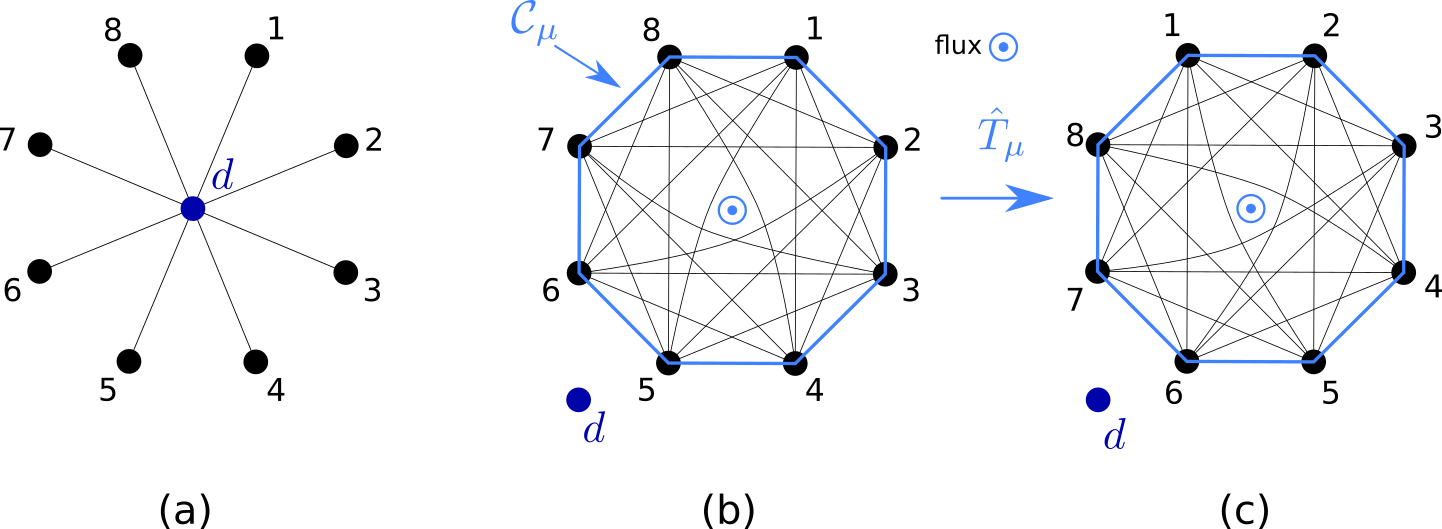
\includegraphics[scale=0.68]{plt/stargraph-to-alltoall}
%\caption{This figure shows the comparison and mapping between the stargraph degenerate ground states and the states of the quantum fluctuation resolved all to all model.}
%\label{fig:stargraph-to-alltoall}
%\end{figure}
%Thus one can see that the ground state degeneracy of the stargraph model with different $J^z$ values gets lifted in the quantum fluctuation resolved all-to-all model. Depending on the value of the flux there is an unique ground state labeled by the $J^z$ value. Tuning the fluc one can go from one ground state to the other. This shows how one can explore different degenerate ground states of the parent stargraph model via the insertion of flux in the corresponding quantum fluctuation resolved all-to-all effective Hamiltonian.



%\subsubsection{Local mott-liquid}
Impurity-bath quantum fluctuation resolved all-to-all effective Hamiltonian is written in terms of the spinor spin operators which are individually made out of two electronic degree of freedom. This is defined as $\vec{S}_i=\frac{\hbar}{2} \displaystyle\sum_{\substack{ \alpha,\beta\in \{\uparrow,\downarrow\}}}  c_{0\alpha}^{(i)\dagger} \vec{\sigma}_{\alpha\beta} c_{0\beta}^{(i)}$. In the above eq.\eqref{eq:all-to-all_1} we see the $U(1)$ symmetry of the effective Hamiltonian. Using the spinor repersentation one can see the spin creation operation in terms of the electronic degree of freedom is 
\begin{eqnarray}
S_i^+ &=& \frac{\hbar}{2} \displaystyle\sum_{\alpha,\beta\in \{\uparrow\downarrow\}} c_{0\alpha}^{(i)\dagger} {\sigma}^{+}_{\alpha\beta} c_{0\beta}^{(i)}
% = \frac{\hbar}{2} \displaystyle\sum_{\alpha,\beta\in \{\uparrow\downarrow\}} c_{0\alpha}^{(i)\dagger}   c_{0\beta}^{(i)} \delta_{\uparrow,\alpha} \delta_{\downarrow,\beta} 
=\frac{\hbar}{2} c_{0\uparrow}^{(i)\dagger} c_{0\downarrow}^{(i)}  \\
S_i^z &=& \frac{\hbar}{2} \displaystyle\sum_{\alpha,\beta\in \{\uparrow\downarrow\}} c_{0\alpha}^{(i)\dagger} {\sigma}^{z}_{\alpha\beta} c_{0\beta}^{(i)} =\frac{\hbar}{2} (c_{0\uparrow}^{(i)\dagger} c_{0\uparrow}^{(i)} - c_{0\downarrow}^{(i)\dagger} c_{0\downarrow}^{(i)} )~,~~~~
\end{eqnarray}
Thus this spinor spins are nothing but the Anderson pseudospin formulation in the spin channel. The spin creation opertor ($S_i^+$) shows simultaneous creation of an electron-hole pair at the realspace origin of the $i^{th}$ channel. The condensation of such electron-hole pais has already been shown in [CITE: mott]. Thus for this effective Hamiltonian one can define twist-translation oeprations to construct the gauge theory and unveiling any hidden degeneracy. Let's recall the effective Hamiltonian
\begin{eqnarray}
H_{eff} &=& \frac{\beta_{\uparrow}(\alpha,\omega_{\uparrow})}{4} \bigg[ \displaystyle\sum_{ij} S_i^+S_j^- ~+ \textrm{h.c.} \bigg]~,
\end{eqnarray}
where $i,j$ are the channel indices. Due to the all-to-all nature of the connectivity one can draw total $K!$ possible unique closed paths ($\mathcal{C}_{\mu}$) where each nodes (channels) is being touched only once. One can thus define total $K!$ number of translation operators ($\hat{T}_{\mu}$) which keeps the Hamiltonian invariant. Let's define one of such translation operator $\hat{T}_{\mu}$ thich gives a periodic shifts along the closed path $\mathcal{C}_{\mu}$. Let's define twist operator along the path $\mathcal{C}_{\mu}$
\begin{eqnarray}
\hat{\mathcal{O}}_{\mu} &=& \exp({i\frac{2\pi}{K} \displaystyle\sum_{\substack{j=1\\ \mathcal{C}_{\mu}}}^{K} j S_j^z} )~,~~\hat{T}_{\mu}=e^{i\hat{P}^{cm}_{{\mu}}}
\end{eqnarray}
The  operation of the translation operator $\hat{T}_{\mu}$ is defined as $\hat{T}_{\mu} S_j^z = S_{j+1}^z$ where $j+1$ and $j$ are the nearest neighbor on the closed path $\mathcal{C}_{\mu}$. Then the braiding rule between the twist and translation operators are give as
\begin{eqnarray}
\hat{T}_{\mu}\hat{\mathcal{O}}_{\mu} \hat{T}^{\dagger}_{\mu} \hat{\mathcal{O}}_{\mu}^{\dagger}  &=&  \exp\{i[2\pi S_1^z-\frac{2\pi}{K}S^z]\} \nonumber\\
&=& \exp\{i[\pm \pi - \frac{2\pi}{K} S^z]\} =\exp(i\frac{2\pi p}{q})
\end{eqnarray}
The availability of the non-trivial braiding staatistics between these twist and translation operators is possible if $p\neq 0$ and $q\neq \infty$. Further simplification leads to the condition
\begin{eqnarray}
 \pm\pi -\frac{2\pi}{K} S^z = \frac{2\pi p}{q} ~~ &\Rightarrow & \pm\frac{1}{2}-\frac{S^z}{K} = \frac{p}{q} \nonumber\\
&& \frac{(\pm K-2S^z)}{2K} = \frac{p}{q}~,~
\end{eqnarray} 
$p,q$ are mutual prime, We knwo that the $S^z$ can take values $(\mp K/2\pm m)$ where $m$ is a integer $0 \leq m \leq K$. Putting this value in the above equation leads to two possible solutions.
\begin{eqnarray}
\frac{(K-m)}{K} &=& \frac{p}{q} ~,~~ \frac{-m}{K}=\frac{p}{q}
\end{eqnarray}
For the first case $K-m=p$ we can see that $m=K$ makes $p$ trivial hus the allowed values are $m=0,\cdots,K-1$, which represents the corresponding $S^z$ eigen values 
\begin{eqnarray}
&&-K/2,-K/2+1,\cdots,K/2-2,K/2-1
\end{eqnarray}
Similarly the second case implies, $-m=p$, but $p=0$ is not allowed as this makes the braiding statistics trivial, thus the possible $S^z$ values are 
\begin{eqnarray}
&&\hspace{2.2cm} -K/2+1,-K/2+2,\cdots,K/2-1,K/2
\end{eqnarray}

\noindent Thus we get the general braiding statistics between the twist and the translation 
\begin{eqnarray}
\hat{T}_{\mu}\hat{\mathcal{O}_{\mu}} \hat{T}^{\dagger}_{\mu}\hat{\mathcal{O}_{\mu}}^{\dagger} &=& e^{i\frac{2\pi p}{K}}
\end{eqnarray}
where $p$ corresponds to different $S^z$ states, related as $p=\pm K/2-S^z$. Thus we can see that there are $K$ possible $S^z$ plaleau states in the all-to-all model where each plateaux is $K$ fold degenerate. This $p/K$ is similar to the filling factor of the fractional quantum Hall effect. There are possibly $K!$ pairs of twist and translation operator corresponding to different closed paths $\mathcal{C}_{\mu}$ which can probe this degeneracy.

\subsubsection{Action on the Hamiltonian}
Now we findout the action of these twist operators on the Hamiltonian. The Hamiltonian is written as 
\begin{eqnarray}
H_{eff}&=& \frac{\beta_{\uparrow}(\alpha,\omega_{\uparrow})}{2} (S^{x2} +S^{y2})   
\end{eqnarray}
Due the all-to-all nature of the effetive Hamiltonian one can find $K!$ possible relative arrangement of those $K$ channels which keeps the Hamiltonian invariant. Here we briefly discuss the choice of the closed loop $\mathcal{C}_{\mu}$ and the insertion of the flux. As shown in the Fig.\ref{fig:stargraph-to-alltoall}(b) we have chosen a particular closed path which crosses all the outer spin only once. We embed that closed loop on a plane and put the flux perpendiculr to the plane through the closed loop. One can find a different closed loop where the ordering of the outer spins will be different. The action of the translation operator shifts the outer spins along this closed curve by one step.

The action of the twist operator on the $S^x$ is determined in the follwoing calculation
\begin{eqnarray}
\hat{O}_{\mu} S^x \hat{O}^{\dagger}_{\mu} &=& \exp({i\frac{2\pi}{K} \displaystyle\sum_{\substack{j=1\\ \mathcal{P}_{\mu}}}^{K} j S_j^z} )S^x \exp({-i\frac{2\pi}{K} \displaystyle\sum_{\substack{j=1\\ \mathcal{P}_{\mu}}}^{K} j S_j^z} ) \nonumber\\
&=& e^{X} S^x e^{-X}
\end{eqnarray}
For simplicity of thte calculation we define $i\frac{2\pi}{K}=\Omega$, thus $X=\Omega\sum_j jS^z_j$. Thus we get
\begin{eqnarray}
e^X S^x e^{-X}&=& S^x+[X,S^x] + \frac{1}{2!}[X,[X,S^x]] +\cdots  \nonumber\\
&=& \sum_l ( S^x_l \cos \theta_l -  S_l^y \sin \theta_l ) ~,~~~\theta_l=\frac{2\pi l}{K}~~~~\\
e^X S^y e^{-X}&=& \sum_l  (S^y_l \cos\theta_l  + S^x_l \sin\theta_l)
\end{eqnarray}
As already defined, $\theta_l=\frac{2\pi l}{K}=\frac{2\pi (K-n)}{K}$, where $n$ is an integer. We can see that in the large channel limit $\theta_l $ becomes inter multiple of $2\pi$. Thus in the large channel limit
\begin{eqnarray}
&& \lim_{K\rightarrow \infty}\hat{\mathcal{O}}_{\mu} H_{eff} \hat{\mathcal{O}}_{\mu}^{\dagger}\nonumber\\
 &=& \frac{\beta_{\uparrow}(\alpha,\omega_{\uparrow})}{2} \bigg[ \hat{\mathcal{O}}_{\mu} S^x \hat{\mathcal{O}}_{\mu}^{\dagger} \hat{\mathcal{O}}_{\mu} S^x \hat{\mathcal{O}}_{\mu}^{\dagger}  + \hat{\mathcal{O}}_{\mu} S^y \hat{\mathcal{O}}_{\mu}^{\dagger} \hat{\mathcal{O}}_{\mu} S^y \hat{\mathcal{O}}_{\mu}^{\dagger}  \bigg]\nonumber\\
&=&\frac{\beta_{\uparrow}(\alpha,\omega_{\uparrow})}{2} \bigg[  S^{x2}+S^{y2}  \bigg] = H_{eff} \nonumber\\
&&\lim_{K\rightarrow \infty } [\hat{\mathcal{O}},H_{eff}] = 0
\label{eq:hamiltonian_twisted}
\end{eqnarray}
 
\noindent The translation operator $\hat{T}_{\mu}=e^{i\hat{\mathcal{P}}_{\mu}}$ commutes with the Hamiltonian thus the generator $\hat{\mathcal{P}}_{\mu}$ also commutes with the Hamiltonian. We can label the $j^{th}$ state with the eigenvalues of this operator $\hat{\mathcal{P}_{\mu}}$ as $|p^{j}_{\mu}\rangle$. We here discuss the action of these twist and translation operators on these states.
\begin{eqnarray}
\hat{T}_{\mu} |p^j_{\mu} \rangle &=& e^{i\hat{\mathcal{P}}_{\mu}} |p^j_{\mu} \rangle = e^{ip^j_{\mu}} |p^j_{\mu}\rangle \nonumber\\
\hat{T}_{\mu} \hat{\mathcal{O}}_{\mu} |p^j_{\mu} \rangle &=&  \hat{\mathcal{O}}_{\mu} \hat{T}_{\mu} e^{i\frac{2\pi m}{K}} |p^j_{\mu}\rangle~~, \nonumber\\
&&~~\textrm{here $m$ signifies different $S^z$ plateaux.} \nonumber\\ \nonumber\\
&=& \hat{\mathcal{O}}_{\mu}   e^{i(\frac{2\pi m}{K}+p_{\mu}^j)} |p^j_{\mu}\rangle~,~~ \frac{2\pi m}{K} \equiv p_{\mu}^{m} \nonumber\\
\hat{T}_{\mu} \bigg( \hat{\mathcal{O}}_{\mu} |p^j_{\mu} \rangle  \bigg) &=& e^{i(p_{\mu}^{m}+p_{\mu}^j)} \bigg( \hat{\mathcal{O}}_{\mu}    |p^j_{\mu}\rangle \bigg)    
\end{eqnarray}
Thus we can see that  $\hat{\mathcal{O}}_{\mu} |p^j_{\mu} \rangle $ is a state of the traslation operator with different eiven value than $|p^j_{\mu} \rangle $, thus orthogonal to each other. Simiarly one can generally show that $\langle p^j_{\mu} | \hat{\mathcal{O}}^{q}_{\mu} |p^j_{\mu} \rangle=0$, where $q$ is any integer. Also in the large $K$ limit we can see from the eq.\eqref{eq:hamiltonian_twisted} that these differnt twisted states has same energy. Which shows that at each plateau state labeled by the $S^z$ eigenvalue has $K$ fold degenerate eigenstates labeled by the eigenvalue of the translation operators. Thus the CSCO is formed by $H,S^z,\hat{T}$. Thus states can be lebeled as  $|E,S^z_j,P^j_{\mu}\rangle$. 




\section{Effect of conduction bath excitations on the fixed point theory}
\subsection{Non-Fermi liquid signatures in momentum space for 2-channel Kondo}
Obtaining the effective Hamiltonian involves obtaining the low energy excitations on top of the ground state of the star graph. The large-energy excitations are ones that involve spin flips. This guides the separation of the Hamiltonian into a diagonal and an off-diagonal piece:
\begin{align}
	H = H_d + V = \underbrace{H_0 + J S_d^z s_\text{tot}^z}_{H_d} + \underbrace{\frac{J}{2}S_d^+ s_\text{tot}^- + \text{h.c.}}_{V + V^\dagger}
\end{align}
We define \(V\) as the interaction term that decreases \(s_\text{tot}^z\) by 1: \(V \ket{s_\text{tot}^z} \to \ket{s_\text{tot}^z - 1}\). Similarly, we define \(V^\dagger \ket{s_\text{tot}^z} \to \ket{s_\text{tot}^z + 1}\). The effective Hamiltonian that has the states \(\ket{S_d^z, s_\text{tot}, s_\text{tot}^z}\) as eigenstates are
\begin{widetext}
\begin{align}
	H_\text{eff} = H_d + V \frac{1}{E_\text{gs} - H_d}V = H_d + \frac{J}{2}S_d^+ s_\text{tot}^- \frac{1}{E_\text{gs} - J S_d^z s_\text{tot}^z - H_0}\frac{J}{2}S_d^- s_\text{tot}^+ +\frac{J}{2}S_d^- s_\text{tot}^+ \frac{1}{E_\text{gs} - J S_d^z s_\text{tot}^z - H_0}\frac{J}{2}S_d^+ s_\text{tot}^-
\end{align}
This is obtained from the Schrodinger equation for the ground state. If we expand the ground state in terms of \(\ket{S_d^z, s_\text{tot}, s_\text{tot}^z}\), we have  \(\ket{\Psi_\text{gs}} = \sum_{S_d^z, s_\text{tot},s_\text{tot}^z}C_{S_d^z, s_\text{tot},s_\text{tot}^z}\ket{S_d^z, s_\text{tot}, s_\text{tot}^z}\). The Schrodinger equation for the ground state can be written as
\begin{align}
	E_\text{gs}\ket{\Psi_\text{gs}} = H \ket{\Psi_\text{gs}} = \left(H_d + V\right)\ket{\Psi_\text{gs}} \implies \left(E_\text{gs} - H_d\right)\sum C_{S_d^z, s_\text{tot},s_\text{tot}^z}\ket{S_d^z, s_\text{tot}, s_\text{tot}^z} = V\sum C_{S_d^z, s_\text{tot},s_\text{tot}^z}\ket{S_d^z, s_\text{tot}, s_\text{tot}^z}
\end{align}
\end{widetext}
\(E_\text{gs}\) is the ground state energy, and can be replaced by the star graph ground state energy if we remove the kinetic energy cost via normal ordering: \(E_\text{gs} = -\frac{J}{2}\left(\frac{K}{2}+1\right) \). Since the interaction part \(V\) only changes \(S_d^z \to -S_d^z\) and \(s^z_\text{tot} \to s^z_\text{tot} \pm 1\), we can simplify the equation into individual smaller equations. For the two-channel model, the possible states are \((s_\text{tot},s^z_\text{tot}) = (0,0), (1,-1), (1,0), (1,1)\). The individual equations for these states are
\begin{align}
	\label{eff_ham_Sdz_10}
	E_\text{gs} \ket{\frac{1}{2}, 1, 0} &= \left(H_d + V \frac{1}{E_\text{gs} - H_d}V^\dagger\right) \ket{\frac{1}{2}, 1, 0}\\
	E_\text{gs} \ket{-\frac{1}{2}, 1, 0} &= \left(H_d + V^\dagger \frac{1}{E_\text{gs} - H_d} V\right) \ket{-\frac{1}{2}, 1, 0}\\
\end{align}
These equations represent the Schrodinger equation for the states \(\ket{S_d^z, 1, 0}\), and the right hand sides therefore give the effective Hamiltonians for those states. If we combine the states into a single subspace \(\ket{1,0}= \left\{\ket{\frac{1}{2}, 1, 0}, \ket{-\frac{1}{2}, 1, 0}\right\}\), the effective Hamiltonian for this composite subspace becomes the sum of the two parts:
\begin{align}
	\label{eff_ham_10}
	H^{1,0}_\text{eff}\ket{1, 0}\bra{1, 0} = \left(H_d + V G_0 V^\dagger + V^\dagger G_0  V\right) \ket{1, 0}
\end{align}
where \(G_0 = \left(E_\text{gs} - H_d\right)^{-1}\). If we expand the subspace as \(\ket{1,0} = \ket{\frac{1}{2}, 1, 0} + \ket{-\frac{1}{2}, 1, 0}\), we recover eqs.~\ref{eff_ham_Sdz_10}. Solving similarly for the other states gives
\begin{align}
	H^{1,1}_\text{eff}\ket{1,  1}\bra{1,  1} &= \left(H_d + V^\dagger G_0  V\right) \ket{1,  1}\\
	H^{1,-1}_\text{eff}\ket{1, - 1}\bra{1, - 1} &= \left(H_d + V G_0 V^\dagger\right) \ket{1, - 1}
\end{align}

To calculate these effective Hamiltonians, we will calculate the individual terms. We can easily simplify the \(S_d^z\) in the denominator of \(G_0\), because \(S_d^\pm \frac{1}{A + B S_d^z} = S_d^\pm \frac{1}{A \mp \frac{1}{2}B}\):
\begin{align}
	V G_0 V^\dagger = \frac{J^2}{4} s_\text{tot}^- \frac{\frac{1}{2} + S_d^z}{E_\text{gs} + \frac{J}{2} s_\text{tot}^z - H_0} s_\text{tot}^+ \\
	V^\dagger G_0 V = \frac{J^2}{4} s_\text{tot}^+ \frac{\frac{1}{2} - S_d^z}{E_\text{gs} - \frac{J}{2} s_\text{tot}^z - H_0} s_\text{tot}^-
\end{align}
Since \(H_0\) does not commute with the spin operators, we will need to expand the denominator to make sense of this Hamiltonian.
\begin{widetext}
\begin{align}
	 V G_0 V^\dagger =  s_\text{tot}^- \frac{1}{E_\text{gs} + \frac{J}{2} s_\text{tot}^z}\left[1 + \frac{1}{E_\text{gs} + \frac{J}{2} s_\text{tot}^z}H_0 + \frac{1}{E_\text{gs} + \frac{J}{2} s_\text{tot}^z}H_0\frac{1}{E_\text{gs} + \frac{J}{2} s_\text{tot}^z}H_0 + \ldots\right] s_\text{tot}^+\\
	 V^\dagger G_0 V =  s_\text{tot}^+ \frac{1}{E_\text{gs} - \frac{J}{2} s_\text{tot}^z}\left[1 + \frac{1}{E_\text{gs} - \frac{J}{2} s_\text{tot}^z}H_0 + \frac{1}{E_\text{gs} - \frac{J}{2} s_\text{tot}^z}H_0\frac{1}{E_\text{gs} - \frac{J}{2} s_\text{tot}^z}H_0 + \ldots\right] s_\text{tot}^-
\end{align}
\end{widetext}
This is an expansion in \(H_0^n/J^{n+1}, n=0,1,2,\ldots\). Expanding up to \(n=2\) and keeping at most two particle interaction terms, 
the effective Hamiltonians for these states are:
\begin{widetext}
\begin{align}
	H_\text{eff}^{1, 1} &= H_0 + J S_d^z + \frac{J^2}{4}\frac{2}{E_\text{gs}}\left[1 + \frac{H_0}{E_\text{gs}} + \frac{s^+_\text{tot}X_{1,\text{tot}}}{2 E_\text{gs}} + \frac{H_0^2 }{E_\text{gs}^2} - \frac{Z_{1,\text{tot}} H_0}{E_\text{gs}^3}\right] \left(\frac{1}{2} - S_d^z\right) \\
	H_\text{eff}^{1, -1} &= H_0 - J S_d^z + \frac{J^2}{4}\frac{2}{E_\text{gs}}\left[1 + \frac{H_0}{E_\text{gs}}  - \frac{s^-_\text{tot}X^\dagger_{1,\text{tot}}}{2 E_\text{gs}}  + \frac{H_0^2}{E_\text{gs}^2}  - \frac{ Z_{1,\text{tot}} H_0}{E_\text{gs}^3}\right] \left(\frac{1}{2} + S_d^z\right) \\
	H_\text{eff}^{1, 0} &= H_0 + \frac{J^2}{2\left(E_\text{gs} + \frac{J}{2}\right)}\left[1 + \frac{ H_0 + \left(\frac{1}{2} + S_d^z\right) s^+_\text{tot}X_{1,\text{tot}} - \left(\frac{1}{2} - S_d^z\right) s^-_\text{tot}X^\dagger_{1,\text{tot}}}{2 \left(E_\text{gs} + \frac{J}{2}\right)} + \frac{H_0^2}{\left(E_\text{gs} + \frac{J}{2}\right)^2} - \frac{Z_{1,\text{tot}} H_0}{\left(E_\text{gs} + \frac{J}{2}\right)^3} \right]
\end{align}
\end{widetext}
We employed the definitions \(X_{n,\text{tot}} \equiv  \sum_l \sum_{k,k^\prime}\left(\epsilon_k - \epsilon_{k^\prime}\right)^n c^\dagger_{k \downarrow}c_{k^\prime \uparrow},  X_{n,l}\) and \( Z_{1,\text{tot}} \equiv \sum_{k,k^\prime,l}\left( \epsilon_k - \epsilon_{k^\prime} \right) \frac{1}{2}\left(c^\dagger_{k \uparrow,l}c_{k^\prime \uparrow,l} - c^\dagger_{k \downarrow,l}c_{k^\prime \downarrow,l}\right)\). Focusing on the effective Hamiltonian for \(\left( 1,0 \right) \), we see lots of non-Fermi liquid terms of the form \(s^+_\text{tot}X_{1,\text{tot}}, s^-_\text{tot}X^\dagger_{1,\text{tot}},Z_{1,\text{tot}} H_0\). These arise because of the degenerate manifold and the increased availability of states in the Hilbert space for scattering, as compared to the unique singlet ground state of the single-channel Kondo model.





%\subsection{Real space non-Fermi liquid effective Hamiltonian for 2-channel Kondo}
%\noindent Here we start with the low energy zero mode fixed point Hamiltonian for the two-channel Kondo obtained under URG treatment. Our goal here is to add excitations on top of this ground state and using the perterbation theory. In doing so we consider the leading order scatter apprearing in the lowest order in the perturbative expansion. Note, in the fixed point zero mode Hamiltonian impurity spin is coupled with the bath electrons via spin exchange coupling, there is no charge exchange coupling present. 
%\begin{eqnarray}
%H^{(2)}&=& \alpha \vec{S}_{imp}.(\vec{S}_1+\vec{S}_2)~~,~~\vec{S}_i =  \frac{1}{2}~ c_{i,\alpha}^{\dagger}~ \vec{\sigma}_{\alpha,\beta}~ c_{i,\beta}
%\label{eq:channel-2-spin}
%\end{eqnarray}
%Here $\vec{S}_i=1,2$ represents the spin degree of freedom present in the origin of the $i^{th}$ channel. Thus one can rewrite the Eq.\eqref{eq:channel-2-spin} interms of the electronic degree of freedom as,
%\begin{eqnarray}
%&&\mathcal{H}_0= H_{0_1}+H_{0_2} \nonumber\\
%&=&\sum_{i=\{1,2\}}\bigg[ \alpha S^z_{imp}. (n_{i,\uparrow}-n_{i,\downarrow})/2 + \frac{1}{2}  ( S_{imp}^{+} c^{\dagger}_{i,\downarrow} c_{i,\uparrow} + \textrm{h.c.}  )\nonumber \bigg]
%\end{eqnarray}
%Here the basis we are interested in is $\{\mathcal{B}\}=\{|S^z_{imp},n_{1,\uparrow},n_{1,\downarrow},n_{2,\uparrow},n_{2,\downarrow}\rangle \}$. In this basis we write down all $2^3=8$ states of the spin Hamiltonian eq.\eqref{eq:channel-2-spin}
%First the two degenerate ground states with energy $-\alpha= E_{\alpha_0}= E_{\alpha_1}$ is given as,
%\begin{eqnarray}
%|\alpha_0\rangle &=& \frac{1}{\sqrt{6}} \bigg[2|\Downarrow,1,0,1,0\rangle-|\Uparrow,0,1,1,0\rangle-|\Uparrow,1,0,0,1\rangle\bigg] \nonumber\\
%|\alpha_1\rangle &=& \frac{1}{\sqrt{6}} \bigg[2|\Uparrow,0,1,0,1\rangle-|\Downarrow,1,0,0,1\rangle-|\Downarrow,0,1,1,0\rangle\bigg] \nonumber
%\end{eqnarray}
%The doubly degenerate lowestlying excited state has energy $E_{\beta_1}=E_{\beta_2}=0$.
%\begin{eqnarray}
%|\beta_0\rangle &=& \frac{1}{\sqrt{2}}\bigg[|\Downarrow,1,0,0,1\rangle-|\Downarrow,0,1,1,0\rangle \bigg] \nonumber\\
%|\beta_1\rangle &=& \frac{1}{\sqrt{2}} \bigg[ |\Uparrow,1,0,0,1\rangle-|\Uparrow,0,1,1,0\rangle \bigg]
%\end{eqnarray}
%Above these two excited states there are another dengenerate excited state manifold with energy $ E_{\gamma_0}=E_{\gamma_1}=E_{\gamma_2}=E_{\gamma_3}=\frac{\alpha}{2}$.
%\begin{eqnarray}
%|\gamma_{0}\rangle &=&\frac{1}{\sqrt{3}} \bigg[|\Uparrow,0,1,0,1\rangle+|\Downarrow,1,0,0,1\rangle+|\Downarrow,0,1,1,0\rangle \bigg] \nonumber\\
%|\gamma_{1}\rangle &=& \frac{1}{\sqrt{3}}\bigg[ |\Uparrow,1,0,0,1\rangle+|\Uparrow,0,1,1,0\rangle+|\Downarrow,1,0,1,0\rangle \bigg] \nonumber\\
%|\gamma_{2}\rangle &=& |\Uparrow,1,0,1,0\rangle~,~~|\gamma_{3}\rangle = |\Downarrow,0,1,0,1\rangle 
%\end{eqnarray}
%Note this spin Hamiltonian has total $8$ states, where ground state is double degenerate with energy $-\alpha$ and the lowest exicites state with energy $0$ is also double degnerate and the second excited state with energy $\alpha/2$ is 4-fold degenerate. 
%\par On top of the zero mode spin-channel interactions we want to consider the effect of the momentum space kinetic energy term $\sum_{k}\epsilon_k (n_{1,k}+n_{2,k})$. We assume identical dispersion for both the channels. Our zero mode spin Hamiltonian is written in the real space, thus it will be easier to do the perterbation theory on the real space. The fourier transformation of the momentum space kinetic energy  term leads to real space hopping term. For simplicity we will be considering the neareast neighbor hoppings between sites within each channels. The real space hopping contributino to the Hamiltonian $H_X$ with the hooping strength is 
%\begin{eqnarray}
%H_{X} &=& -t \displaystyle\sum_{\substack{<1,l_1> \\ <2,l_2>}} (c^{\dagger}_{1,\sigma}c_{l_1,\sigma}+c^{\dagger}_{2,\sigma}c_{l_2,\sigma}+ ~\textrm{h.c.})
%\end{eqnarray}
%Here $l_i$ represents the nearest site to the origin of the $i^{th}$ channel. Thus here we are interested in studying the Hamiltonian $\mathcal{H}_0+H_X$. The perterbating term $H_x$ contains scattering which takes the states of the zero mode Hamltonain out of spin-channel scattering space. Thus befor we start the perturbation theroy we must expand the basis of the zero mode Hamiltonian itself. Thus the basis which contains the nearest neighbor sites of both the channels is given as 
%\begin{eqnarray}
%&&\{\mathcal{B}_{extnd}\} \equiv  \{\mathcal{B}\} \otimes  \{|n_{l_1,\uparrow},n_{l_1,\downarrow},n_{l_2,\uparrow},n_{l_2,\downarrow}\rangle\} \\
%&=& \{|S^z_{imp},n_{1,\uparrow},n_{1,\downarrow},n_{2,\uparrow},n_{2,\downarrow}\rangle \otimes |n_{l_1,\uparrow},n_{l_1,\downarrow},n_{l_2,\uparrow},n_{l_2,\downarrow}\rangle\} \nonumber
%\end{eqnarray}
%Note there are $2^4=16$ elements in the subspace $\{|n_{l_1,\uparrow},n_{l_1,\downarrow},n_{l_2,\uparrow},n_{l_2,\downarrow}\rangle\}$. In the spin-channel basis $\{\mathcal{B}\}$ there $2$ degenerate ground states. Because the unpurterbed Hamiltonian $\mathcal{H}_0$ has no scattering terms outside the spin sector, in the extended basis $\{\mathcal{B}_{extnd}\}$ the total ground state deneracy becomes simply $2\times 2^4$, $32$ fold. Thus the total hamiltonian we are interested in is 
%\begin{eqnarray}
%\mathcal{H} &=& \frac{\alpha\hbar}{2}~ \vec{S}_d. \displaystyle\sum_{i=\{1,2\}} \displaystyle\sum_{\alpha,\beta\in\{\uparrow,\downarrow\}}c_{i\alpha}^{\dagger} \vec{\sigma}_{\alpha\beta} c_{i\alpha} +H_X
%%-t\displaystyle\sum_{i=\{1,2\}}\displaystyle\sum_{\substack{\langle i,l_i \rangle\\ \sigma}}(c^{\dagger}_{i,\sigma} c_{l_i,\sigma}+ \textrm{h.c.}) 
%%\\
%%&=& \displaystyle\sum_{i=1,2} \bigg[ \alpha\hbar~ \vec{S}_d. \vec{S}_i -t\displaystyle\sum_{\substack{\langle i,l_i \rangle\\ \sigma}}(c^{\dagger}_{i,\sigma} c_{l_i,\sigma}+ \textrm{h.c.}) \bigg] \nonumber\\
%%&=& \mathcal{H}_0+H_X
%\label{eq:excitation_hamiltonian}
%\end{eqnarray}
%There are two degenrate states $|\alpha_1\rangle$ and $|\alpha_2\rangle$. Thus the two degenerate ground states in the above basis is give as,
%\begin{eqnarray}
%|\tilde{\alpha}_0\rangle &=&| {\alpha}_0\rangle\otimes |n_{l_1,\uparrow},n_{l_1,\downarrow},n_{l_2,\uparrow},n_{l_2,\downarrow}\rangle \\
%|\tilde{\alpha}_1\rangle &=& | {\alpha}_1\rangle\otimes |n_{l_1,\uparrow},n_{l_1,\downarrow},n_{l_2,\uparrow},n_{l_2,\downarrow}\rangle
%\end{eqnarray}
%Using degenerate perturbation theory we calculate the first and the second order corrections to the Hamiltonian. The first order and the second order low energy effective Hamiltonian is given as 
%\begin{eqnarray}
%H^{(1)} &=& \sum_{ij} |\alpha_i\rangle \langle \alpha_i  | V| \alpha_j \rangle \langle \alpha_j |~\nonumber\\
%H^{(2)} &=& \sum_{ij} \sum_l |\alpha_i\rangle \frac{\langle \alpha_i  | V| \mu_l \rangle \langle \mu_l  | V| \alpha_j \rangle}{E_0-E_{l}}\langle \alpha_j |
%\end{eqnarray}
%where $|\alpha_i\rangle$ represents the ground states with energy $E_0$ and $\mu_l$ represents the ecvited states with energy $E_l$. One can easily check the diagonal term in effective Hamiltonain coming from the $1^{st}$ or any $odd$ order correction is zero as the state never returns to the original starting state via odd number of scatterings. For the case of first order it is easy to see that the off-diagonal correction to the effective Hamiltonian is also zero. Thus the lowest order where we expect the non-zero corrections is the second order. We first calculate the diagonal correction in the first order
%\begin{eqnarray}
%H^{(2)}_{diag} &=& \sum_{i} \sum_l |\alpha_i\rangle\langle \alpha_i | \frac{|\langle \alpha_i  | V| \mu_l \rangle|^2 }{E_0-E_{l}}
%\end{eqnarray}
%As single scattering always takes the state outside of the spin-channel, the state $V|\alpha_i\rangle$ is an excited state with energy $0$ ($=E_l$). This $\alpha_i$ representing the ground state can take total $32$ configurations as discussed. Out of this $32$ states $| {\alpha}_0\rangle\otimes |n_{l_1,\uparrow},n_{l_1,\downarrow},n_{l_2,\uparrow},n_{l_2,\downarrow}\rangle$ can take $16$ configurations and $| {\alpha}_1\rangle\otimes |n_{l_1,\uparrow},n_{l_1,\downarrow},n_{l_2,\uparrow},n_{l_2,\downarrow}\rangle$ can take the rest 16 configurations. Note the two degnereate states $|\tilde{\alpha}_0\rangle$  and $|\tilde{\alpha}_1\rangle$ is labeled by the $J^z$ eigenvalue $\pm 1/2$ respectively, where $J^z$ is the total z-component of the impurity and zero modes of the baths. Thus these $32$ ground states can be seperated in two 16 state groups labeled by the $J^z=\pm 1/2$ eigenvalues. For the $J^z=1/2$ sector we get the effective Hamiltonian
%\begin{eqnarray}
%H^{(2)}_{diag} (1/2) &=& \frac{2t^2}{E_0} \hat{I} - \frac{2t^2}{3E_0} ( S_{l_1}^z + S_{l_2}^z)
%%= \frac{2t^2}{E_0} \hat{I} - \frac{4t^2}{3E_0} \bigg[S_{l_1}^z+S_{l_2}^z\bigg]
%\end{eqnarray}
%Similarly the for $J^z=-1/2$ we get 
%\begin{eqnarray}
%H^{(2)}_{diag} (-1/2) &=& \frac{2t^2}{E_0} \hat{I} + \frac{2t^2}{3E_0} (S_{l_1}^z+S_{l_2}^z)
%%= \frac{2t^2}{E_0} \hat{I} + \frac{4t^2}{3E_0} \bigg[S_{l_1}^z+S_{l_2}^z\bigg]
%\end{eqnarray}
%where $S_{l_i}^z=(n_{l_i\uparrow}-n_{l_i\downarrow})/2.$ This above result shows that the diagonal correlation to the LEH coming from the ground states $J^z=\pm 1/2$ has a emergent field term. 
%\begin{eqnarray}
%H^{(2)}_{diag} &=& -4t^2 \hat{I}
%\end{eqnarray}
%But the total contribution shows the trivial nature of the diagonal part in the LEH. This clearly shown that there is no Fermi liquid terms present in low energy in the 2-channel Kondo problem. Here, $\hat{I}$ is the identity operator made out of all $2^4=16$ possible number operator combinations as shown below
%\begin{eqnarray}
%\hat{I} &=& \sum_{\hat{o}=\hat{n},(1-\hat{n})} \hat{o}_{l_1,\uparrow}\hat{o}_{l_1,\downarrow} \hat{o}_{l_2,\uparrow}\hat{o}_{l_2,\downarrow}
%\end{eqnarray}
%Due to the ground state degeneracy in the 2-channel problem, there are possible quantum scattering within the ground state manifold among those degenerate states. This leads to a low energy effective Hamiltonian which is offdiagonal in nature as shown below,
%\begin{eqnarray}
%H_{NFL}&=&H^{(2)}_{off} = \sum_{i\neq j} \sum_l |\alpha_i\rangle \frac{\langle \alpha_i  | V| \mu_l \rangle \langle \mu_l  | V| \alpha_j \rangle}{E_0-E_{l}}\langle \alpha_j | \nonumber\\
%&=& -\frac{8t^2}{3} [ (S_1^z)^2 c_{2\uparrow}^{\dagger}c_{2\downarrow}  (  c_{l_1\uparrow}c_{l_1\downarrow}^{\dagger} +  c_{l_2\uparrow}c_{l_2\downarrow}^{\dagger}  ) \nonumber\\
%&+& (S_2^z)^2 c_{1\uparrow}^{\dagger}c_{1\downarrow}  (  c_{l_1\uparrow}c_{l_1\downarrow}^{\dagger} +  c_{l_2\uparrow}c_{l_2\downarrow}^{\dagger}  ) ] + \textrm{h.c.} ~,~~~~
%\label{eq:hamiltonian_NFL}
%\end{eqnarray}
%This LEH is purely a non-Fermi liquid. The emergenec of non-Fermi liquid is primarily coming due to the degenerate ground states present in the stargraph problem in the absence of the realspace hopping terms. One can see that though there was no prior inter channel direct interactions, the LEH shows the emergence of such terms through correlated quantum scatterings. 
%
%
%\subsection{Presence of a marginal Fermi liquid: Orthogonality catastrophe in two-channel MCK model}
%At the stable fixed point \(J ^* = J_1^* = \frac{2}{K \rho}\), the ground states of the Hamiltonian are those of the star graph model, with a degeneracy of \(K\). We now specialise to the two-channel Kondo model. To find the low-energy excitations on top of this ground state manifold, we insert a tight-binding nearest-neighbour hopping between the zeroth site (the one that holds the impurity) and the first site (site that's nearest to the zeroth site) as a perturbation and calculate the diagonal and off-diagonal terms generated by this perturbation. It is found that when we trace out the impurity, we are left only with real space off-diagonal terms:
%\begin{equation}\begin{aligned}
%	\label{nfl_terms}
%	V_\text{eff} = \frac{2t^2}{J^*}\left[\left(\sigma^z_{0,1}\right)^2 s^+_{0,2} + \left(\sigma^z_{0,2}\right)^2 s^+_{0,1}\right] \left(s^-_{1,1} + s^-_{1,2}\right) + \text{h.c.}
%\end{aligned}\end{equation}
%where \(\sigma^z_{0,l} = \hat n_{0\uparrow,l} - \hat n_{0\downarrow,l}, s^+ = c^\dagger_{0 \uparrow,l}c_{0 \downarrow,l}\) and \(s^- = \left(s^+\right)^\dagger\). The notation \(0\sigma,l\) has the site index \(i=0,1,2,\ldots\) as the first label, the spin index \(\sigma=\uparrow,\downarrow\) as the second label and the channel index \(l=1,2\) as the third index.
%
%These are the terms that are generated because of the presence of the impurity. Such a non-Fermi liquid (NFL) contribution to the effective Hamiltonian and the absence of any Fermi-liquid term at the same order should be contrasted with the local Fermi liquid excitations induced by the singlet ground state of the single-channel Kondo model~\cite{nozieres1974fermi,wilson1975renormalization,hewson1993}. We wish to point out that such NFL terms were also obtained by Coleman, et al.~\cite{Coleman_tsvelik} in terms of Majorana fermions at the zeroth site and the first site of the \(\sigma-\tau\) version of the two-channel Kondo model. They then went on to compute a single-particle self-energy renormalisation coming from this NFL term that matches the phenomenological~\cite{varma2002singular} and microscopic forms of the marginal Fermi liquid self-energy~\cite{anirbanmott1,anirbanurg1}. We take a different route in order to calculate the self-energy contribution coming from Eq.~\ref{nfl_terms}.
%
%In the URG analysis of the 2D Hubbard model at half-filling~\cite{anirbanurg1}, it was found that the normal phase of the Mott insulator was a metal with properties that have been phenomenologically attributed to the marginal Fermi liquid. The excitations of such a phase are described by a two particle-one hole composite object:
%\begin{equation}\begin{aligned}
%	\label{mfl_urg}
%	H_\text{MFL} = \sum_{k,k^\prime,k^{\prime\prime},\sigma}R \hat n_{k\sigma} \hat n_{k^\prime \overline\sigma}\left(1 - \hat n_{k^{\prime\prime}\sigma}\right) 
%\end{aligned}\end{equation}
%We wish to look for such a term in the effective Hamiltonian. For this, we will perform a perturbative treatment of the hopping at strong coupling \(J \to \infty\) where the perturbative coupling \(t^2/J\) is arbitrarily small and again obtain Eq.~\ref{nfl_terms}. Such a change from the strong coupling model with parameter \(J\) to a weak coupling model with parameter \(t^2/J\) amounts to a duality transformation~\cite{kroha_kolf_2007,zitko_fabrizio_2017}. It can be shown that the duality transformation leads to an identical MCK model~\cite{kroha_kolf_2007} (self-duality), which implies we can have identical RG flows, and our transformation simply extracts the NFL piece from the dual model. The self-duality also ensures that the critical intermediate-coupling fixed point is unique and can be reached from either of the models.
%
%The diagonal part of eq.~\ref{nfl_terms} is
%\begin{equation}\begin{aligned}
%	V_\text{eff} = \frac{2t^2}{J}\sum_{l=1,2}\left(\sum_\sigma \hat n_{0\sigma,l}\right) s^+_{0,\bar l}s^-_{1,\bar l} + \text{h.c.}
%\end{aligned}\end{equation}
%where \(\bar l = 3 - l\) is the channel index complementary to \(l\). We will fourier transform this effective Hamiltonian into \(k-\)space. The NFL part becomes
%\begin{equation}\begin{aligned}
%	\label{k_space_od}
%	\sum_{\sigma, \left\{k_i,k_i^\prime\right\},l} \frac{2t^2}{J}e^{i\left(k_1 - k_1^\prime\right)a}c^\dagger_{k\sigma,l}c_{k^\prime\sigma,l}c^\dagger_{k_2 \uparrow, \bar l}c_{k_2^\prime \downarrow,\bar l}c^\dagger_{k_1 \downarrow,\bar l}c_{k_1^\prime \uparrow, \bar l} + \text{h.c.} 
%\end{aligned}\end{equation}
%This form of the Hamiltonian is very similar to the three-particle interaction term in Appendix B of~\cite{anirbanmott1}. The channel indices in Eq.~\ref{k_space_od} can be mapped to the normal directions in~\cite{anirbanmott1}. As specualted eariler, the 2 particle-1 hole interaction in Eq.~\ref{k_space_od} has a diagonal component which can be obtained by setting \(k=k^\prime, k_1 = k_2^\prime\) and \(k_2 = k_1^\prime\):
%\begin{equation}\begin{aligned}
%	H_\text{eff,MFL} = \sum_{k, k_1, \atop{k_2,\sigma,  l}} \frac{2t^2e^{i\left(k_1 - k_2\right)a}}{J} \hat n_{k\sigma,l} \hat n_{k_2 \uparrow, \bar l}\left(1 - \hat n_{k_1 \downarrow,\bar l}\right) + \text{h.c.}\\
%	= \sum_{k, k_1, \atop{k_2,\sigma,  l}} \frac{4t^2}{J} \cos a\left(k_1 - k_2\right)  \hat n_{k\sigma,l} \hat n_{k_2 \uparrow, \bar l}\left(1 - \hat n_{k_1 \downarrow,\bar l}\right)
%\end{aligned}\end{equation}
%The most dominant contribution comes from \(k_1 = k_2 = k^\prime\), revealing the non-Fermi liquid metal~\cite{cox_jarrell_two_channel_rev,andrei_jerez_1995}:
%\begin{equation}\begin{aligned}
%	\label{mfl_large}
%	H^*_\text{eff,MFL} = \frac{4t^2}{J} \sum_{\sigma, k, k^\prime, l} \hat n_{k\sigma,l} \hat n_{k^\prime \uparrow, \bar l}\left(1 - \hat n_{k^\prime \downarrow,\bar l}\right)
%\end{aligned}\end{equation}
%Following~\cite{anirbanmott1}, one can follow the RG evolution of the dual coupling \(R_j = \frac{4t^2}{J_j}\) at the \(j^\text{rh}\) RG step, in the form of the URG equation
%\begin{equation}\begin{aligned}
%	\Delta R_j =- \frac{R_j^2}{\omega - \epsilon_{j}/2 - R_j/8}
%\end{aligned}\end{equation}
%In the RG equation, \(\epsilon_{j}\) represents the energy of the \(j^\text{th}\) isoenergetic shell. It is seen from the RG equation that \(R\) is relevant in the range of \(\omega < \frac{1}{2}\epsilon_j\) that has been used throughout, leading to a fixed-point at \(R^*/8 = \omega - \frac{1}{2}\epsilon^*)\). The relevance of \(R\) is expected because the strong coupling \(J\) is irrelevant and \(R \sim 1/J\).
%
%The renormalisation in \(R\) leads to a renormalisation in the single-particle self-energy~\cite{anirbanmott1}. The \(k-\)space-averaged self-energy renormalisation is
%\begin{equation}\begin{aligned}
%	\Delta \Sigma(\omega) = \rho {R^*}^2\int_0^{\epsilon^*} \frac{d\epsilon_j}{\omega - \epsilon_j/2 + R_j/8}
%\end{aligned}\end{equation}
%The density of states can be approximated to be \(N^*/R^*\), where \(N^*\) is the total number of states over the interval \(R^*\). As suggested by the fixed point value of \(R_j\), we can approximate its behaviour near the fixed point by a linear dependence of the dispersion \(\epsilon_j\). The two limits of the integration are the start and end points of the RG. We start the RG very close to the Fermi surface and move towards the fixed point \(\epsilon^*\). Near the start point, we substitute \(\epsilon = 0\) and \(R = \omega\), following the fixed point condition. From the the fixed point condition, we also substitute \(R^*/8 = \omega - \frac{1}{2}\epsilon^*\). On defining \(\bar \omega = N^* \left(\omega - \frac{1}{2}\epsilon^*\right)\), we can write
%\begin{equation}\begin{aligned}
%	\label{self_energy}
%	\Delta \Sigma(\omega) \sim  \bar \omega \ln \frac{N^* \omega}{\bar \omega}
%\end{aligned}\end{equation}
%The self-energy also provides the quasiparticle residue for each channel\cite{anirbanmott1}:
%\begin{equation}\begin{aligned}
%	Z(\bar\omega) = \left(2 - \ln \frac{2\bar\omega}{N^* \omega}\right) ^{-1}
%\end{aligned}\end{equation}
%\textit{As the energy scale \(\omega \to 0\), the \(Z\) vanishes, implying that the ground state and lowest-lying excitations, in the presence of the NFL terms, are not adiabatically connected to the Fermi gas. This is the orthogonality catastrophe~\cite{varma2002singular,anderson_infraredcat,yamada_catastrophe,yamada1979orthogonality} in the two-channel Kondo problem, and it is brought about by the presence of the terms in Eq.~\ref{mfl_large}}. Such terms were absent in the single-channel Kondo model, because there was no multiply-degenerate ground state manifold that allowed scattering. This line of argument shows that the extra degeneracy of the ground state subspace and the frustration of the singlet order that comes about when one upgrades from the single-channel Kondo model to the MCK models is at the heart of the NFL behaviour, and the orthogonality catastrophe should be a general feature of all such frustrated MCK models. A local NFL term with a self-energy of the form in eq.~\ref{self_energy} was also obtained in the \(\sigma-\tau\) model by Coleman et al.~\cite{Coleman_tsvelik}. The common features show the universality between the two-channel Kondo and the \(\sigma-\tau\) models.
\subsection{Low temperature thermodynamic behaviour}
\noindent In order to understnad this non-Fermi liquid we calculate some thermodyanmic quantities like impurity specific heat and suseptibility. First we calcualte the self energy of this NFL hamiltonian. In the real space one can get a diagonal piece from the above equation by using the Fermionic anticommutation relations.
\begin{eqnarray}
H_{eff}^{off,(2)} |_{diag} &=& -(16t^2/3) [ (S_1^z)^2+ (S_2^z)^2 ]   
\end{eqnarray}
We can find the corresponding momentum space Hamiltonian by doing the fouries transforamtion to the Hamiltonian  $H_{eff}^{off,(2)} |_{diag} $ as.
\begin{eqnarray}
%&&-\frac{16t^2}{3}\bigg[\bigg(\frac{1}{4N} \displaystyle\sum_{k,\sigma} n_{k\sigma}-\frac{1}{2N^2} \displaystyle\sum_{k_1,k_2} n_{k_1\uparrow} n_{k_2\downarrow} \bigg) + \bigg(\frac{1}{4N} \displaystyle\sum_{k,\sigma} \tilde{n}_{k\sigma}-\frac{1}{2N^2} \displaystyle\sum_{k_1,k_2} \tilde{n}_{k_1\uparrow} \tilde{n}_{k_2\downarrow} \bigg) \bigg] \nonumber\\
H_{eff}^{off,(2)} |_{diag}&=& -\frac{4t^2}{3} \frac{1}{N} \bigg[ \displaystyle\sum_{k,\sigma} n_{k\sigma}(1-\frac{1}{N} \displaystyle\sum_{k_2}  n_{k_2,-\sigma}  ) \nonumber\\
&&+ \displaystyle\sum_{k,\sigma} \tilde{n}_{k\sigma} ( 1-\frac{1}{N} \displaystyle\sum_{ k_2} \tilde{n}_{k_2,-\sigma}  ) \bigg]  
\end{eqnarray}
The above relation leads to the correction to the kinetic energy, which is
\begin{eqnarray}
%\bar{\epsilon}_k&=& \epsilon_k+\Sigma_k \nonumber\\
\bar{\epsilon}
_k-\epsilon_k=\Sigma_k 
% -\frac{4t^2}{3N} \bigg(1-\frac{1}{N} \displaystyle\sum_{k_2}  \langle n_{k_2,-\sigma} \rangle \bigg) \nonumber\\
&&= -\frac{4t^2}{3N^2}\bigg(1-\frac{N}{e^{(\epsilon_k-\mu)/k_BT}+1}\bigg)
\label{eq:self-energy-NFL}
\end{eqnarray}
Using the self-energy we calculate the impurity speciftic heat defined as $C_{imp}=C(J^*)-C(0)$ which is defined as
\begin{eqnarray}
C_{imp} &=& \sum_{\Lambda,\sigma} \beta \bigg[ \frac{(\bar{\epsilon}_{\Lambda})^2 e^{\beta \bar{\epsilon}_{\Lambda}}}{( e^{\beta \bar{\epsilon}_{\Lambda}} +1)^2}  -\frac{({\epsilon}_{\Lambda})^2 e^{\beta {\epsilon}_{\Lambda}}}{( e^{\beta {\epsilon}_{\Lambda}} +1)^2} \bigg]
\end{eqnarray}
Here we are intersted in the low temperature behavior of this impurity specific-heat. Using the self-energy obtained above we calculate the impurity susecptibility for $t=0.1$ and $\alpha=1$. 
\begin{figure}
\centering
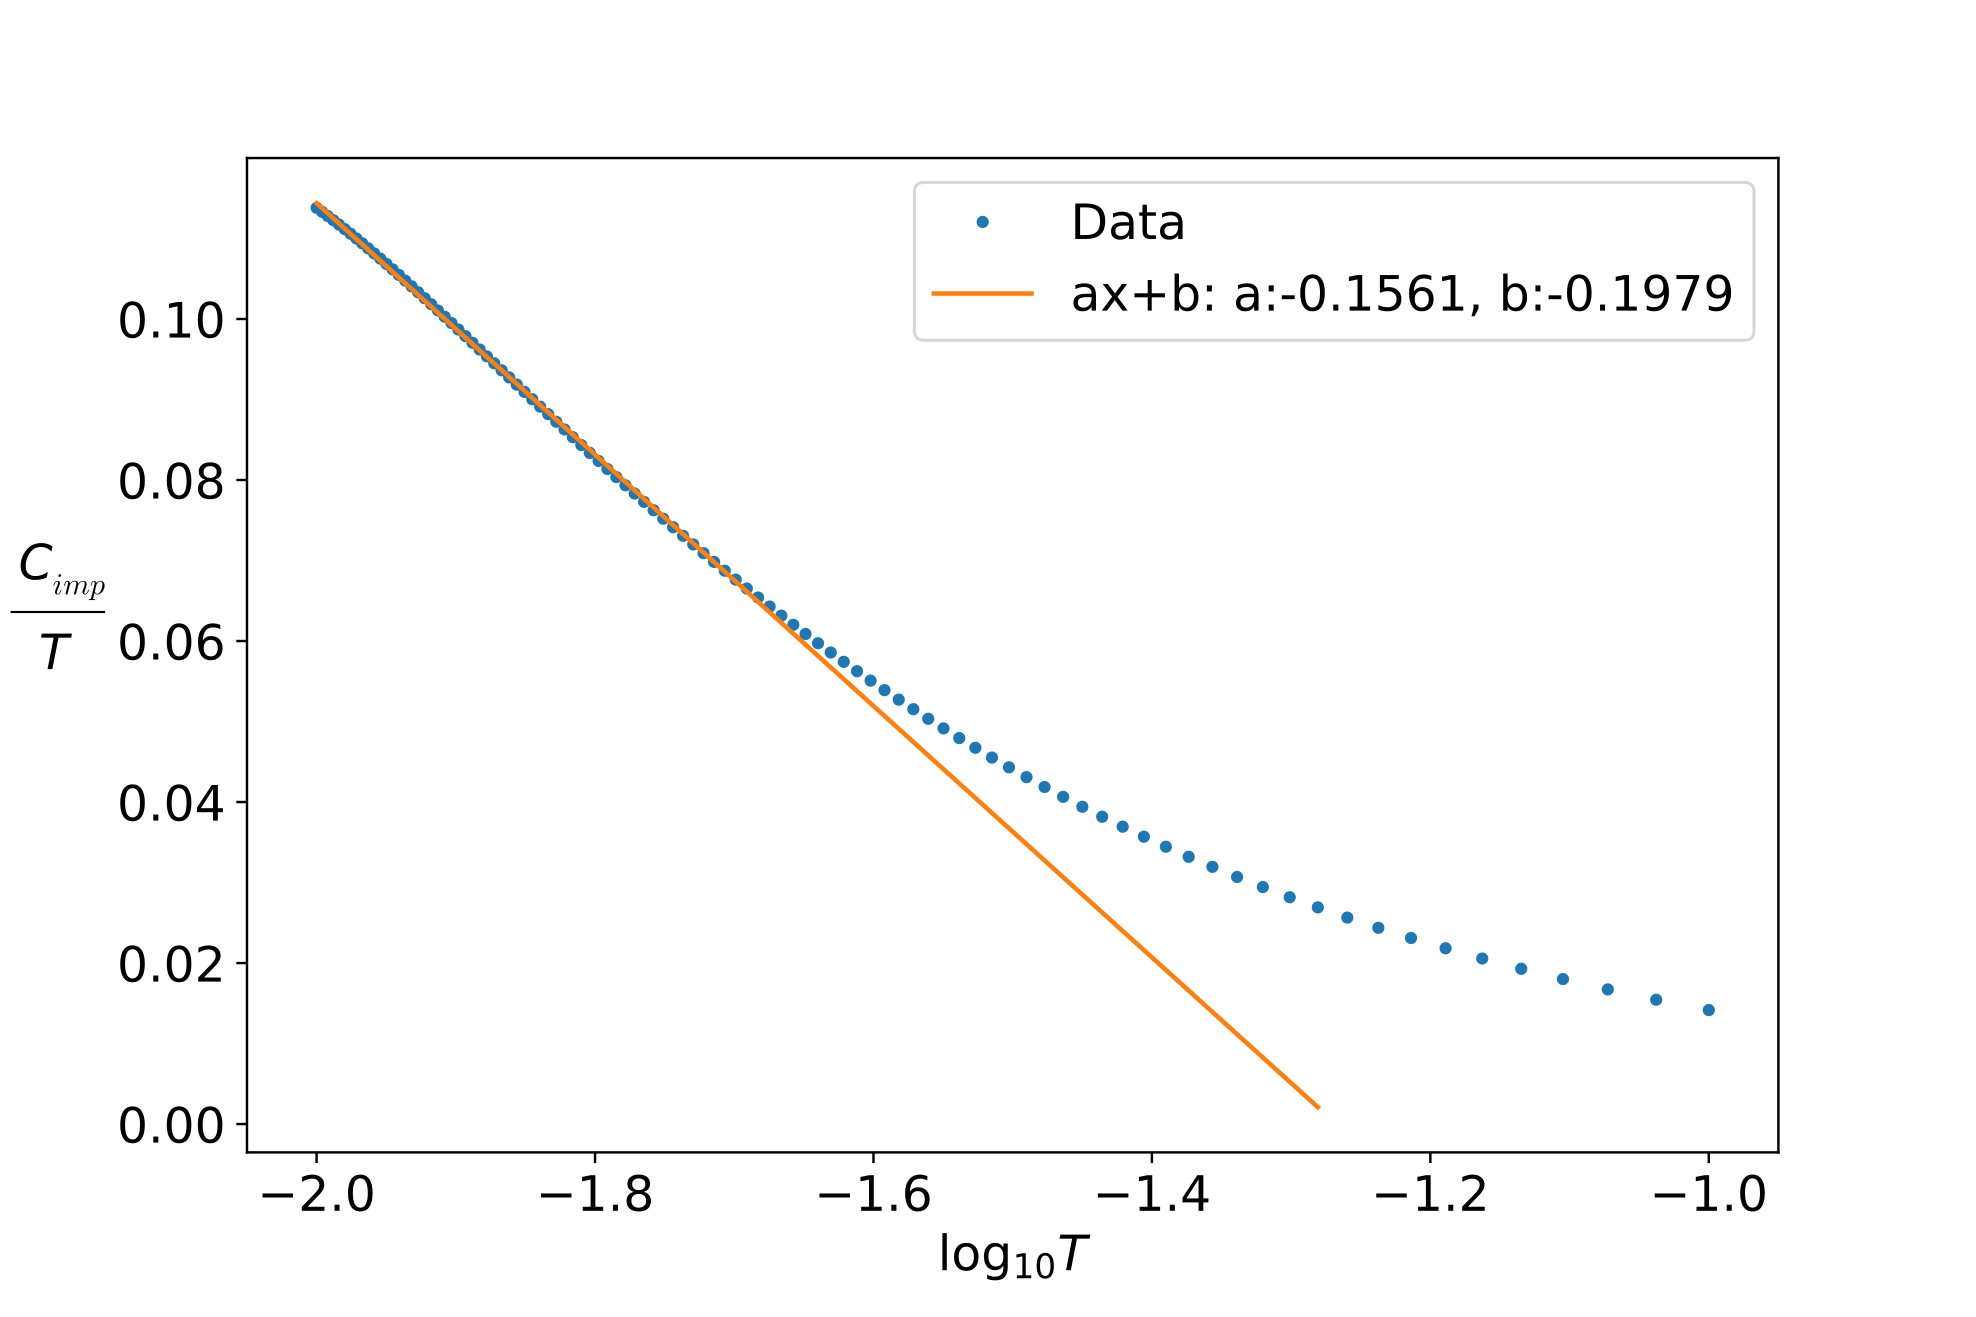
\includegraphics[scale=0.36]{plt/FINAL_fitted_Cv_t_0p1.png}
\caption{This figure shows the variation of the impurity specific heat with the temperature.}
\label{fig:Cv_imp}
\end{figure}
The above Fig.\ref{fig:Cv_imp} shows that at low temperature follows logarithmic behavior for the single channel case which is in agreement with the results known in the literature [CITE].
\begin{eqnarray}
\frac{C_{imp}}{T} \propto \log T
\end{eqnarray}
%\subsubsection{Exact diagonalization}
Apart from this impurity specific heat one can calculate the magnetic susceptibilty. For that we do the exact diagonalizaton of the NFL Hamiltonian eq.\eqref{eq:hamiltonian_NFL} and get the entire eigenspectrum. On all those different state we can calculate teh expectation value of the magnetization squared $\langle (S^z)^2 \rangle$. Using these expectation values we can calculate the suseptibility by using the formula
\begin{eqnarray}
\chi &=& \beta\bigg[\frac{\sum e^{-\beta \bar{\epsilon}_{\Lambda}} \langle \bar{S}^{z2} \rangle}{\sum e^{-\beta \bar{\epsilon}_{\Lambda}} } -\frac{\sum e^{-\beta \epsilon_{\Lambda}} \langle S^{z2 }\rangle }{\sum e^{-\beta \epsilon_{\Lambda}} } \bigg] 
\end{eqnarray}
We numerically compute the $\chi$ from the definition above and study it's dependence on temperature.
\begin{figure}[!h]
\centering
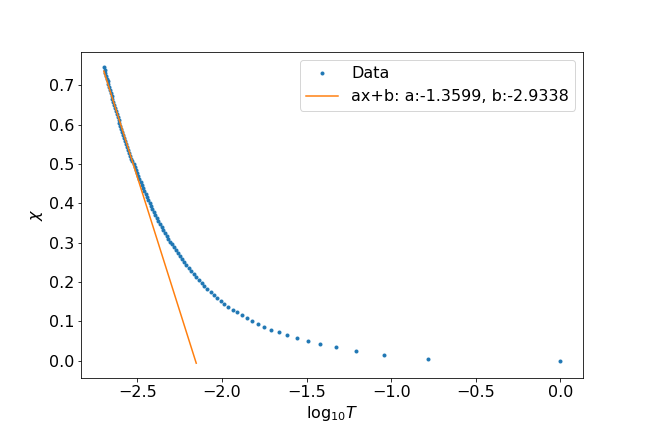
\includegraphics[scale=0.36]{plt/NFL_Chi_log_0p1}
\caption{Suseptibility}
\label{fig:NFL_susecptibility}
\end{figure}
The above figure shows that at low temperture the suseptibility follows the logarithmic behavior.
\begin{eqnarray}
\chi(T) &\propto& \log T
\end{eqnarray}

\noindent As expected both the $C_{imp}/T$ and $\chi$ follows the logarithmic behavior which is known in the literature for the two channel Kondo problem. From the slopes we can calculate the Wilson ratio $C_{imp}/T\chi$, we find that in our case where we have taken upto two nearest neighbors to each zeroth sides of two channels the Wilson ratio is $\approx 8.3$ which is greater than the actual value. For a smaller system with only one nearest neighbor to the zeroth site of both the channels we find the Wilson number if even higher shows that in a larger system the Wilson ratio approaches a smaller value. 
%Direct fourier transformation on the $H^{(2)}_{off}$ leads to the LEH in momentum space showing higher order scattering involving electronic degree of freedoms. For simplicility we only focus on the diagonal piece which is $H_k$ given as
%\begin{eqnarray}
%H_k&=&-\frac{4t^2}{3 N^4} \displaystyle\sum_{\substack{k_1,k_2\in (1),\\ k_3,k_4\in (2)\\ \sigma,\sigma'}} n_{k_1,\sigma} (1-n_{k_2,-\sigma})  \tilde{n}_{k_3,\sigma'} (1-\tilde{n}_{k_4,-\sigma'}) ~,~~~~\nonumber
%\end{eqnarray}
%where (1) and (2) represnts the sets of momentum space points in two channels respectively. The local NFL has a fourth order contribution to the diagonal momentum space density-density interaction, this is a multiplication of MFL terms of two channels. There are lower order contributions also as shown in the above sections.


%Similar to the two channel case, our calculation of the diagonal LEH for the three channel case shown the absence of local Fermi liquid term. In this case we get non-zero contribution from all the three ground states $|J^z=-1\rangle$, $|J^z=0\rangle$ and $|J^z=1\rangle$.
%We get the diagonal contribution to the LEH in the second order is 
%\begin{eqnarray}
%H^{(2)}_{eff, diag} &=& - \frac{7.2 J^2}{\alpha} \hat{I}
%\end{eqnarray}
%The contribution associater to different ground states $|J^z=-1\rangle$, $|J^z=0\rangle$ and $|J^z=1\rangle$ is given respectively as $- \frac{2.4 J^2}{\alpha} \hat{I} + \hat{\mathcal{F}},- \frac{2.4 J^2}{\alpha} \hat{I} ,- \frac{2.4 J^2}{\alpha} \hat{I} - \hat{\mathcal{F} }$,
%\noindent where $\hat{\mathcal{F}}$ is a function of diagonal number oprators of sites nearest neighbor to the zeroth site of each channels. We also get offdiagonal terms in the LEH which is shown below.
%%in the Appendix.\ref{ap:three-channel}. 





\subsection{Three channel LEH}
\noindent Similar to the two channel case, we here calculate the low energy effective Hamiltonain for three channel Kondo problem by introducing the real space hoppting on top of the zero mode three-channel stargraph model. This zero mode three channel stargraph model has three fold degenerate ground states with total $2^4=16$ states in the eigen spectrum. The three degenerate ground states are given as 
\begin{eqnarray}
|\alpha_{-1}\rangle &=& c|1000 \rangle-b (|0100 \rangle + |0010 \rangle+ | 0001 \rangle) \nonumber\\
|\alpha_{+1}\rangle &=& b(|1110 \rangle+ | 1101 \rangle + | 1011 \rangle)-c | 0111 \rangle \nonumber\\
|\alpha_0\rangle &=& -a(|1100 \rangle + |1010\rangle +|1001 \rangle)\nonumber\\
&&~~~~~~~+a(|0110 \rangle+| 0101 \rangle +| 0011\rangle)
\end{eqnarray}
where $a=0.4082482904638638 $, $b=0.2886751345948 $, $c=0.8660254037844386$ \textbf{(PLEASE CHANGE THIS!)}. Here the state is represented by $|n_{d},n_1,n_2,n_3\rangle$, where $n_i=1/0$ represents the spin configuration $S_i^z=\pm 1/2$ respectively. Next we use degenerate perturbation theory to get the LEH which contains diagonal and off-diagonal terms. In this case we get non-zero contribution from all the three ground states $|J^z=-1\rangle$, $|J^z=0\rangle$ and $|J^z=1\rangle$. We get the diagonal contribution to the LEH in the second order to be
\begin{eqnarray}
H^{(2)}_{eff, diag} &=& - \frac{7.2 J^2}{\alpha} \hat{I}
\end{eqnarray}
The contribution associater to different ground states $|J^z=-1\rangle$, $|J^z=0\rangle$ and $|J^z=1\rangle$ is given respectively as $- \frac{2.4 J^2}{\alpha} \hat{I} + \hat{\mathcal{F}},- \frac{2.4 J^2}{\alpha} \hat{I} ,- \frac{2.4 J^2}{\alpha} \hat{I} - \hat{\mathcal{F} }$,
\noindent where $\hat{\mathcal{F}}$ is a function of diagonal number oprators of sites nearest neighbor to the zeroth site of each channels. The off-diagonal terms in the LEH is appearing due to the scattering between pair of degenerate states $(\alpha_0,\alpha_{+1})$ and $(\alpha_0,\alpha_{-1})$, there is no contribution in the second order coming from the scattering between $(\alpha_{-1},\alpha_{+1})$. The effective low energy Hamiltonian in the second ordere is given as

\begin{widetext}
\begin{eqnarray}
H^{(2)}_{eff,off-diag} &=& \sum_{\substack{(ijk)=\\(123),(231),(312)}}\bigg[ c_{i\uparrow}c_{i\downarrow}^{\dagger} \bigg( -2ab \bigg\{ \Sigma_{jk} +c_{j\uparrow}^{\dagger}c_{j\downarrow}c_{k\uparrow}c_{k\downarrow}^{\downarrow} \bigg\} -ac(\Omega_{jk}+\tilde{\Omega}_{jk}) \bigg) + ~~\textrm{h.c.}\bigg] \otimes \hat{\Xi}_l
\end{eqnarray}
\end{widetext}
where different operators are defined as
\begin{eqnarray}
\Sigma_{i,j} &&=n_{i\uparrow}(1-n_{i\downarrow}) (1-n_{j\uparrow})n_{j\downarrow} + (1-n_{i\uparrow})n_{i\downarrow} n_{j\uparrow} (1 -n_{j\downarrow})\nonumber\\
\Omega_{i,j} &=&4S_i^z S_j^z n_{i\uparrow} n_{j\uparrow}\nonumber\\
\tilde{\Omega}_{i,j} &=& 4S_{i}^zS_j^z (1-n_{i\uparrow})(1-n_{j\uparrow}) \nonumber\\
 \hat{\Xi}_l&=&  ( c_{l_1\uparrow}^{\dagger} c_{l_1\downarrow} +c_{l_2\uparrow}^{\dagger} c_{l_2\downarrow} + c_{l_3\uparrow}^{\dagger} c_{l_3\downarrow} + \textrm{h.c.})
\end{eqnarray}


%\section{Entanglement properties}
%
%\subsection{Entanglement properties of the zero mode}
%\noindent Using the above exact wavefunctions we can numerically compute various entanglement properties of this stargraph model. 
%
%\subsubsection{Impurity entanglement entropy}
%\begin{figure}[!h]
%\centering
%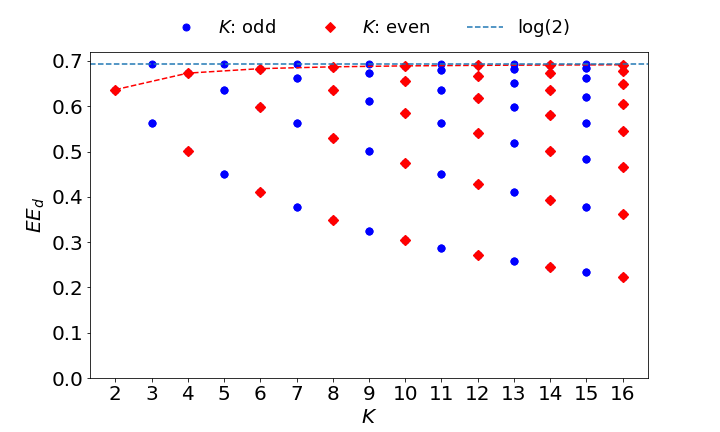
\includegraphics[scale=0.32]{plt/EE_multi_channel_ANN.png}
%\caption{Caption }
%\label{fig:EE_d}
%\end{figure}
%\noindent Here we are interested in finding the entanglement of the central impurity spin with the rest of the multi-channel bath zero mode. For single channel case the the ground state is unique and is $|J=0,J_z=0 \rangle = \frac{1}{\sqrt{2}} (|\uparrow_{d}\downarrow_0\rangle -|\downarrow_d \uparrow_0\rangle)$. Thus, one can easily calculate the reduced density matrix of the impurity by tracing out the $0^{th}$ state. From that reduced denisty matrix the entanglement entropy is $\log 2$, which is maximum possible for a spin-1/2. In the case of multi-channel problem there are $K$ orthogonal set of ground states $|J^z\rangle$, for each such state the entaglement is different. The state $|J^z\rangle \equiv |S_d=1/2,S=K/2;(S-1/2),J^z\rangle$ can be written in the fundamental basis as shown in the Eq.\eqref{eq:wf_fundamental_basis}. Then the density matrix is $\rho=|J^z\rangle\langle J^z|$ from which we can calculate the reduced density matrix by partial tracing the impurity degree of freedom 
%%$\rho_{d}=\textrm{Tr}_{d} \rho=\sum_{S_d^z} \langle S_d^z| \rho | S^z_d\rangle$. 
%\begin{eqnarray}
%\rho_{d}&=& \textrm{Tr}_{d} \rho=\sum_{S_d^z} \langle S_d^z| \rho | S^z_d\rangle ~,~~EE_d = -\rho_{d} \log \rho_{d}~~~
%\end{eqnarray}
%\noindent The eigenvalues of this reduced density matrix given by $\lambda_i$ is called entanglement spectrum. We are interested in the von-Neumann entanglement entropy of the impurity spin with thte rest ($EE_d$). We are intersted in the scaling of this entanglement entropy with the channel number. As shown in the Fig.\ref{fig:EE_d} the x-axis is the channel number and for a particular channel there are may possible entanglement values corresponding to different $J^z$ states. The minimum entanglement entropy state (associated with the $J^z=J$ state) decreases show the classical nature of this maximally polarized state. On the other hand the maximum entanglement entropy (associated with $J^z_{min}$ state) for a particular channel $K$ is saturating to $\log K$ in the large $K$ limit. Another important result that we see, for any odd value of $K$ the minimum entanglement entropy associated with $J^z=0$ is $\log 2$ shows a formation of perfectly entangled state made out of more than 2 spins (e.g; singlet). In this state $|J^z=0\rangle$ all the $K$(odd) outer spins participate in quantum scattering with the central impurity spin in such a way the central spin is maximally entangled which is not the case for any other $J^z$ state. In the large $K$ limit irrespective it's even and odd nature there are always a $J^z_{min}$ state where the central impurity spin is maximally entangled.
%\begin{figure}[!h]
%\centering
%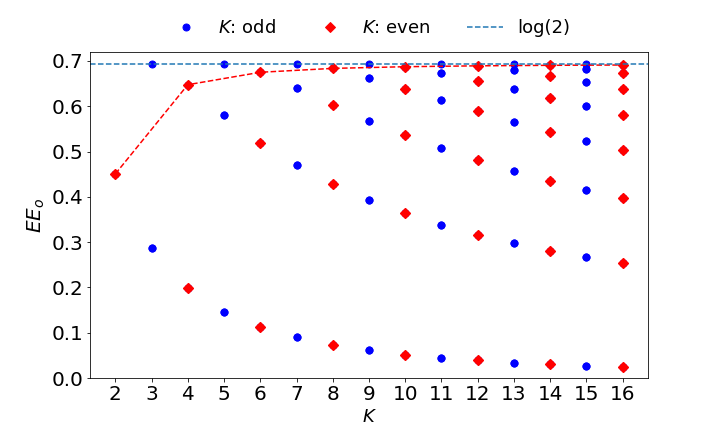
\includegraphics[scale=0.32]{plt/outer_EE_multi_channel_ANN.png}
%\caption{caption}
%\label{fig:EE_outer}
%\end{figure}
%In a $K$ channel system all the outer spins are equivalent (has $Z_N$ symmetry), thus studying the entanglement of any one outer spin with the rest is enough. Here we do a similar entanglement entropy study where we get the reduced density matrix ($\rho_o$) by partial tracing out any one outer spin say the $l^{th}$ ($1\leq l \leq K$) one $S^z_{l}$. 
%\begin{eqnarray}
%\rho_{o} &=& \textrm{Tr}_{l} \rho =\displaystyle\sum_{S^z_{l}} \langle S^z_l | \rho | S^z_{l} \rangle~,~EE_o=-\rho_{o}\log \rho_{o}
%\end{eqnarray}
%We do a similar entanglement scaling with the channel number $K$. We find that minimum entanglement entropy associated with the state $J^z=J$ is approaching zero in the limit $K\gg 1$. In contrast the minimum entanglement entropy associated with $J^z_{min}$ state is saturating at $\log 2$ in the large $K$. Thus in the state $J^z=0$ for any $K$ (or $J^z=\pm 1/2$ for $K\gg 1$) any outer spin is maximally entangled with the rest.
%
%\par The above entanglement studies Fig.(\ref{fig:EE_d},\ref{fig:EE_outer}) show  that for odd channel case there exist a state $J^z=0$ where the central spin $S_d$ and any outer spin $S_i$ is maximally entangled with the rest. This shows the special and unique property of the stargraph ground state where you can create state made out of morethan 2 spins where each any every one is maximally entangled with the rest. Thus this stargraph ground state is very important in the quantum information theory. 
%
%
%%\subsubsection{Macroscopic singlet state}
%%\noindent  The $|J^z=0\rangle_{K} $ state of a $K$(odd) channel stargraph problem can be very genrally written as
%%\begin{eqnarray}
%%|J^z=0\rangle_K &=& \frac{1}{\sqrt{2}} \bigg[ |\Uparrow\rangle_d \otimes |\gamma_{\downarrow}\rangle_K -  |\Downarrow\rangle_d \otimes |\gamma_{\uparrow}\rangle_K \bigg]  
%%\label{eq:maximally_entangled_state}
%%\end{eqnarray}
%%where $|\Uparrow\rangle_d$ and $|\Downarrow\rangle_d$ represents the impurity state $S_d^z=\pm 1/2$ respectively. Let's define $U_{+}$ represents the set of all possible sub-systems of the set $[K]$ with $(K+1)/2$ numbers of elements in it. We define complement of any one set $g\in U_+$ , $g^{c}$ such that $g\cup g^{c}=[K]$.
%%\begin{eqnarray}
%%|\gamma_{\sigma} \rangle_K &=& \frac{1}{\sqrt{{K \choose \frac{K+1}{2}} }} \displaystyle\sum_{\substack{ g\in U_{+} }} \prod_{\substack{i\in g \\j\in g^c}} |\sigma_i\rangle \otimes |\bar{\sigma}_j \rangle~,~ 
%%\end{eqnarray}
%%where $\sigma_i=\pm 1/2$ and $\bar{\sigma}_i=-\sigma_i$, $\pm 1/2$ representing the state $\uparrow_i,\downarrow_i$ respectively for the $i^{th}$ spin. Thus the density matrix for this state $|J^z=0\rangle_K$ can be written as $\rho=|J^z=0\rangle_K \langle J^z=0|_K$. For this state one can simply verify that $\rho_{d}=\textrm{Tr}_d \rho=\frac{1}{2} (|\gamma_{\downarrow}\rangle_K \langle\gamma_{\downarrow}|_K + |\gamma_{\uparrow}\rangle_K \langle\gamma_{\uparrow}|_K)$  which has eigenvalues $1/2,1/2$ leading to the entanglement entropy $S_{d}= \log 2$. Similary one can verify that the entanglement entropy of any other spin with the rest is $\log 2$. Thus all the spins in the state eq.\eqref{eq:maximally_entangled_state} is maximally entangled with the rest representing a macroscopic singlet state with morethan $2$ spins.
%%
%%\par \textit{Add for even channel.}
%
%
%\subsubsection{Mutual Information}
%%/home/sp/RESEARCH ||||||||/BackToCampus||||||||||||||||/_RESEARCH_/Autumn21/PythonA21/StarGraph/2021/Groundstate/plt/NEW31Dec_I_2_vs_Nch_[1, 2].png
%%/home/sp/RESEARCH ||||||||/BackToCampus||||||||||||||||/_RESEARCH_/Autumn21/PythonA21/StarGraph/2021/Groundstate/plt/NEW31Dec_I_2_vs_Nch_[0, 1].png
%
%
%\begin{figure}[!h]
%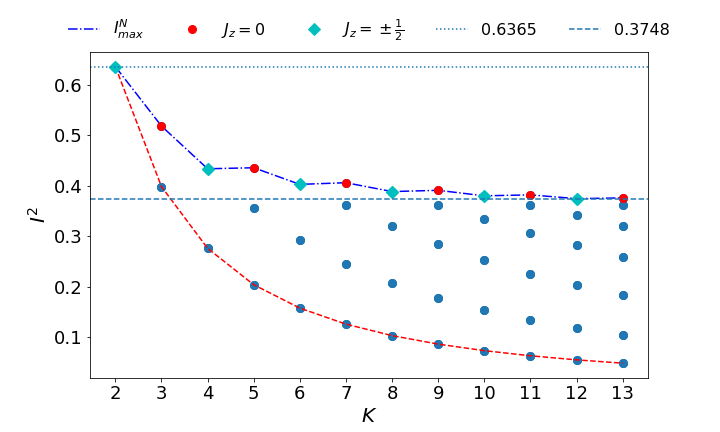
\includegraphics[scale=0.32]{plt/NEW31Dec_I_2_vs_Nch_[0,1]}
%\caption{ds}
%\label{fig:MI_d_o}
%\end{figure}
%\noindent In the above study our focus was on the von-Neumann entanglement entropy, now we are interested in the correlation signatures present in the stargraph grounds states. Mutual inforamtion is one such measure which captures the correlations present between two subsystems (A,B) in a particular state defined as
%\begin{eqnarray}
%I^2(A:B)=S_A+S_B-S_{A\cup B}
%\end{eqnarray}
%where $S_{A}$ is the von-Neumann entanglement entropy of the subsystem $A$ with the rest. Here we are interested in computing two types of mutual inforamtions first, study the mutual information between the impurity-spin and one outer spin $I^2(d:o)$. Because all the outer spins are symmetric, the mutual information between impurity-spin with any one outer spin is same and can capture the correlation between two $A$ and $B$. We have done a scaling study of this mutual information for different channel numbers $K$. As shown in the Fig.\ref{fig:MI_d_o} in the large $K$ limit the maxima of the mutual information associated with the state $J^z_{min}$ is saturating at $0.3748$ and the Mutual information associated with the state $J^z=J$ is decreasing showing the classical limit.
%\begin{figure}[!h]
%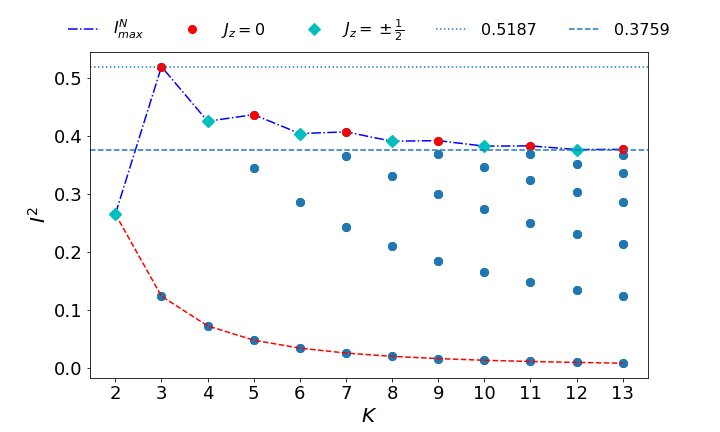
\includegraphics[scale=0.32]{plt/NEW31Dec_I_2_vs_Nch_[1,2]}
%\caption{ds}
%\label{fig:MI_o_o}
%\end{figure}
%Next, we have done a similar study by calculating the mutual information between two outer spin $I^2(o:o)$. In this also we find that the maximum mutual information between any outer spins saturates at the value $0.3759$ very close to the $I^2(d:o)$ case.
%
%\par As can be seen from the above Figure.(\ref{fig:MI_d_o},\ref{fig:MI_o_o}) that  both the maximum mutual information of $I^2(d:o)$ and $I^2(o:o)$ try to saturate near the same value. Thus in the large $K$ limit in the $J^z_{min}$ state mutual information between any two spins in the stargrah model is same saturating at a constant value ($0.37$). Though the difference can be seen in the state $J^z=J$ where the mutual information thus correlation s between two outer spins vanishes in the large $K$ limit faster than the mutual information between the impurity and any one outer spin. Thus correlation wise there is no difference between impurity-outer pair and outer-outer pair in the large $K$ limit.
%
%
%\subsubsection{Multi-partite information}
%\noindent Similar to the mutual inforamtion one can calculate any higher order mutli-partie inforamtion to find the nature of the correlations present in different ground states. We define the tripartite information among three subsystems $A,B,C$ as $I^3_{ABC} = (S_A+S_B+S_C)-(S_{AB}+S_{BC}+S_{CA})+S_{ABC}~$. This tri-parite information scaling with the number of channels $K$ also shown behavior similar to the mutual information case, the highest tri-partite information is associated with the $J^z_{min}$ state and saturating in the limit of $K\gg 1$. One can measure $N-$partite information for a collection of subsystems (CSS) $\{\mathcal{A}\}\equiv\{A_1,A_2,\cdots,A_K\}$. To define the $N-$partite information, we first define the power set of the CSS $\{\mathcal{A}_N\}$ as $\mathcal{P}(\{\mathcal{A}_{N}\})$, and the collection of all subsets of $\mathcal{P}(\{\mathcal{A}_{N}\})$ with $m$ subsystems in it as $\mathcal{B}_m(\{\mathcal{A}_N\})\equiv \{ Q~| ~Q\subset \mathcal{P}(\{\mathcal{A}_{N}\}), |Q|=m \}$. We also define the union and intersection of all the subsystems present in $Q$ as ${V}_{\cup}({Q})\equiv \bigcup_{A\in Q} A$ and ${V}_{\cap}({Q})\equiv \bigcap_{A\in Q} A$ respectively. Finally, the von Neumann entanglement entropy of the subsystem $A$ is given by $S_{A} $. Then the $N-$partite information that we are interested in is defined as
%\begin{eqnarray}
%I^{N}_{\{\mathcal{A}_N\}} &=& \bigg[\displaystyle\sum_{m=1}^{N} (-1)^{m-1} \displaystyle\sum_{Q \in \mathcal{B}_m(\{\mathcal{A}\})} S_{V_{\cup}({Q})} \bigg]- S_{V_{\cap}(\mathcal{A}_N)}~.~~~~
%\label{eq:I_N_definition}
%\end{eqnarray}
%Studying these mutli-partite informations one can understand the nature of the correlations present among the outer spins.
%\begin{figure}
%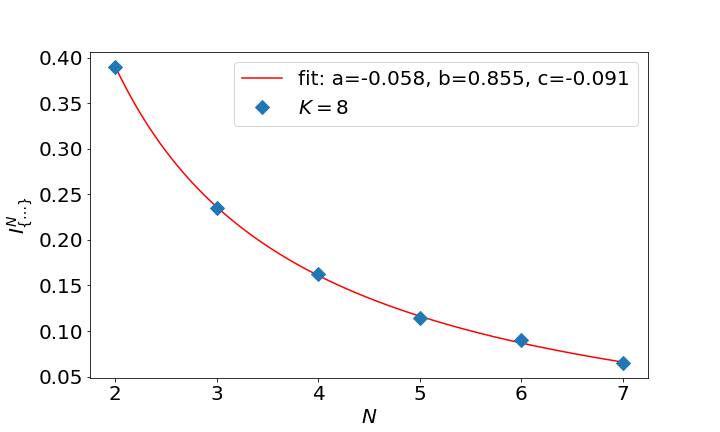
\includegraphics[scale=0.32]{plt/IN_vs_N_K8.png}
%%I_N_vs_N_N9.png}
%\caption{This figure shows how the $m-partite$ information varies with $m$ showing the entanglement distribution amond different number of outer-spins.}
%\label{fig:Im_vs_m}
%\end{figure}
%\noindent Our study of this multi-partite information presented in the above Fig.\eqref{fig:Im_vs_m} shows that the higher oreder multi partite informations decreaseas as you increase the order folloring a power law.
%
%
%
%
%
%\subsection{Entanglement properties in the presence of excitations}
%\begin{figure}[!h]
%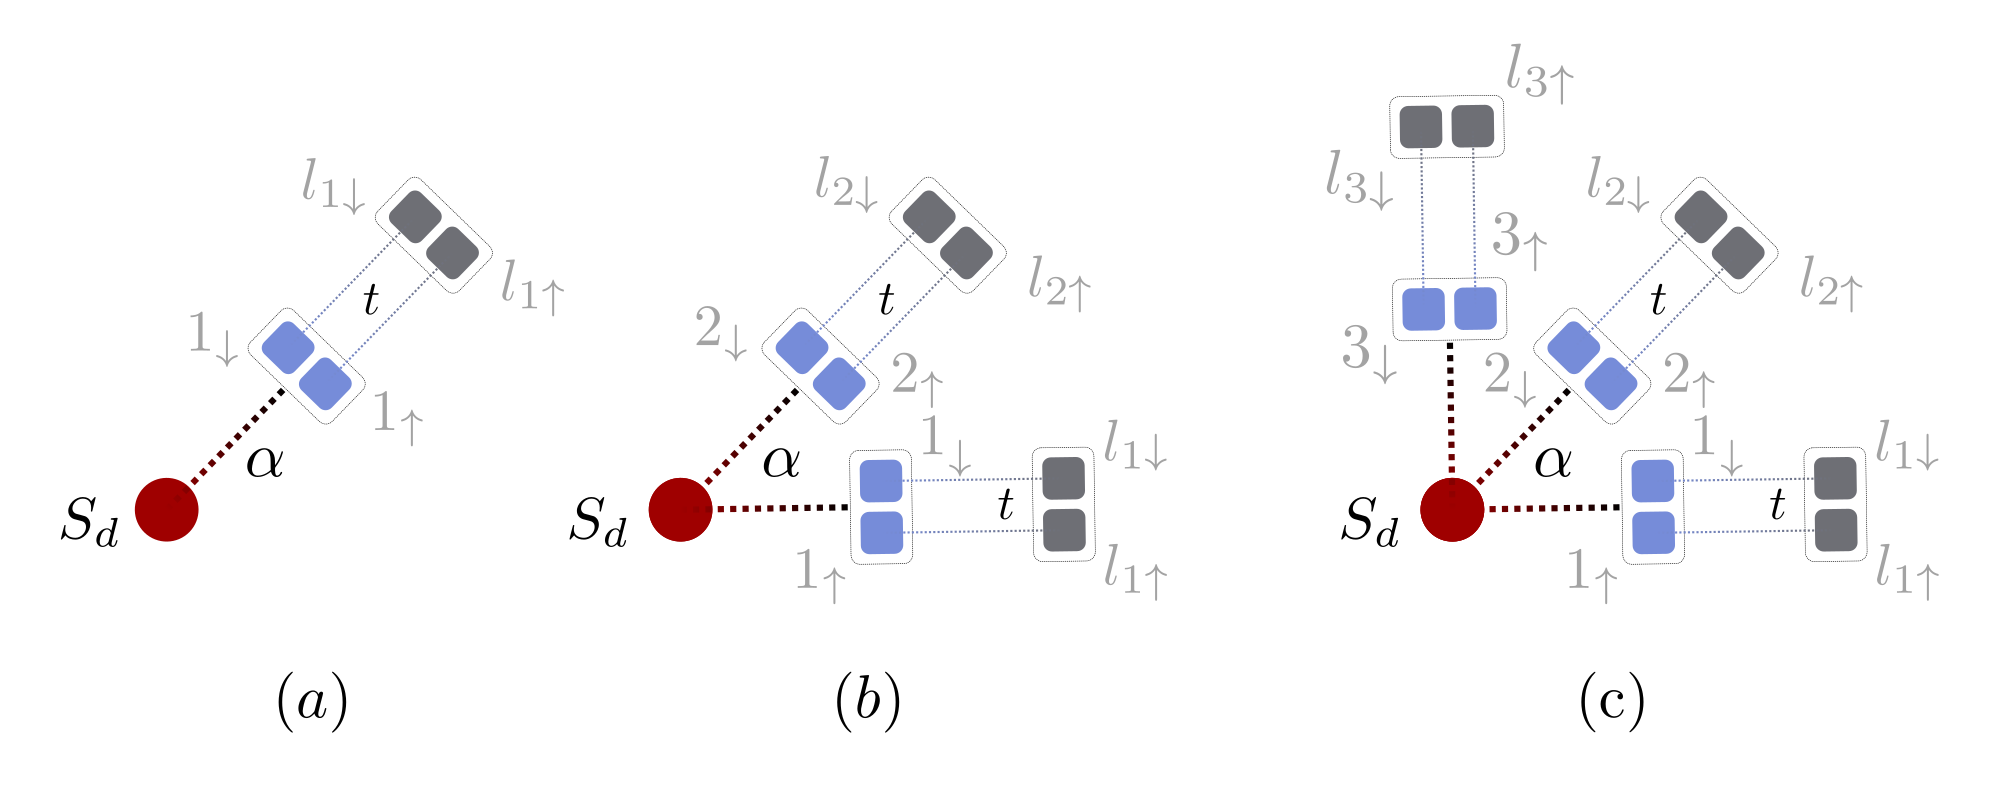
\includegraphics[scale=0.34]{plt/hopping_fock_states}
%\caption{This is a schematic diagram of (a) single channel and (b) two channel problem. $S_d$ is the impurity spin. For more details refer to the text.}
%\label{fig:schematic_hopping}
%\end{figure}
%
%
%\noindent Apart from various thermodynamic properties of the local NFL, here we study the various entanglement signatures present in the ground state. We start with the Hamiltonian Eq.\eqref{eq:excitation_hamiltonian} where we are only taking the nearest neighbor real space hopping (t) where $t=0$ case is the zero mode Hamiltonian of the multi-channel Kondo as shown in the Fig.\ref{fig:schematic_hopping}. In the single channel case the impurity ($S_d$) is talking to the spin degree of freedom at the real space origin ($\{1_{\uparrow},1_{\downarrow}\}$) of the unique conduction bath via a Hisenberg coupling. For $2$ channel case the impurity is talking to $2$ different origins of different conductions channels ($\{1_{\uparrow},1_{\downarrow}\}$ and $\{2_{\uparrow},2_{\downarrow}\}$) and hopping connects to their nearest neighbor sites, for example $\{1_{\uparrow},1_{\downarrow}\}$ connects to $\{l_{1\uparrow},l_{1\downarrow}\}$. Thus, for $K$ channel case we are solving a problem with one spin 1/2 degree of freedom and $2K$ electronic sites. As we increase the hopping strength $t$ from zero to non-zero, the sites of the zero mode Hamiltonian starts to scatter with their respective nearest neighbor sites.
%
%
%\begin{figure}[!h]
%\centering
%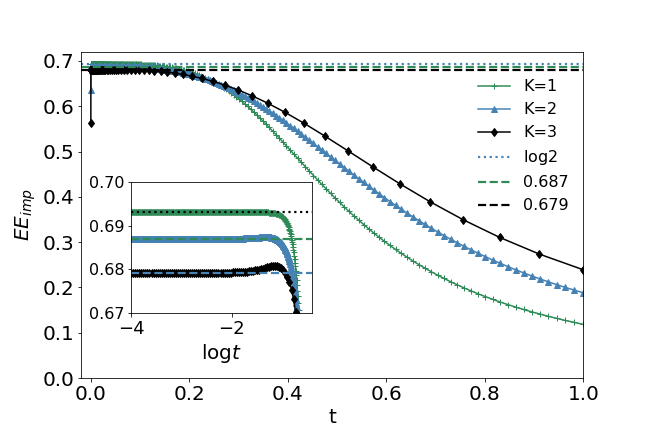
\includegraphics[scale=0.42]{plt/A_I1_ch123_['d']}
%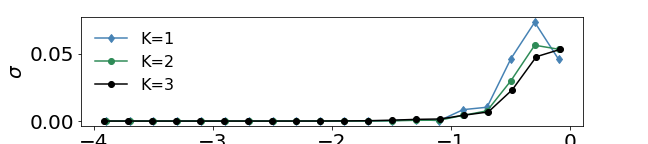
\includegraphics[scale=0.42]{plt/errorbar_A_I1_ch123_['d']}
%%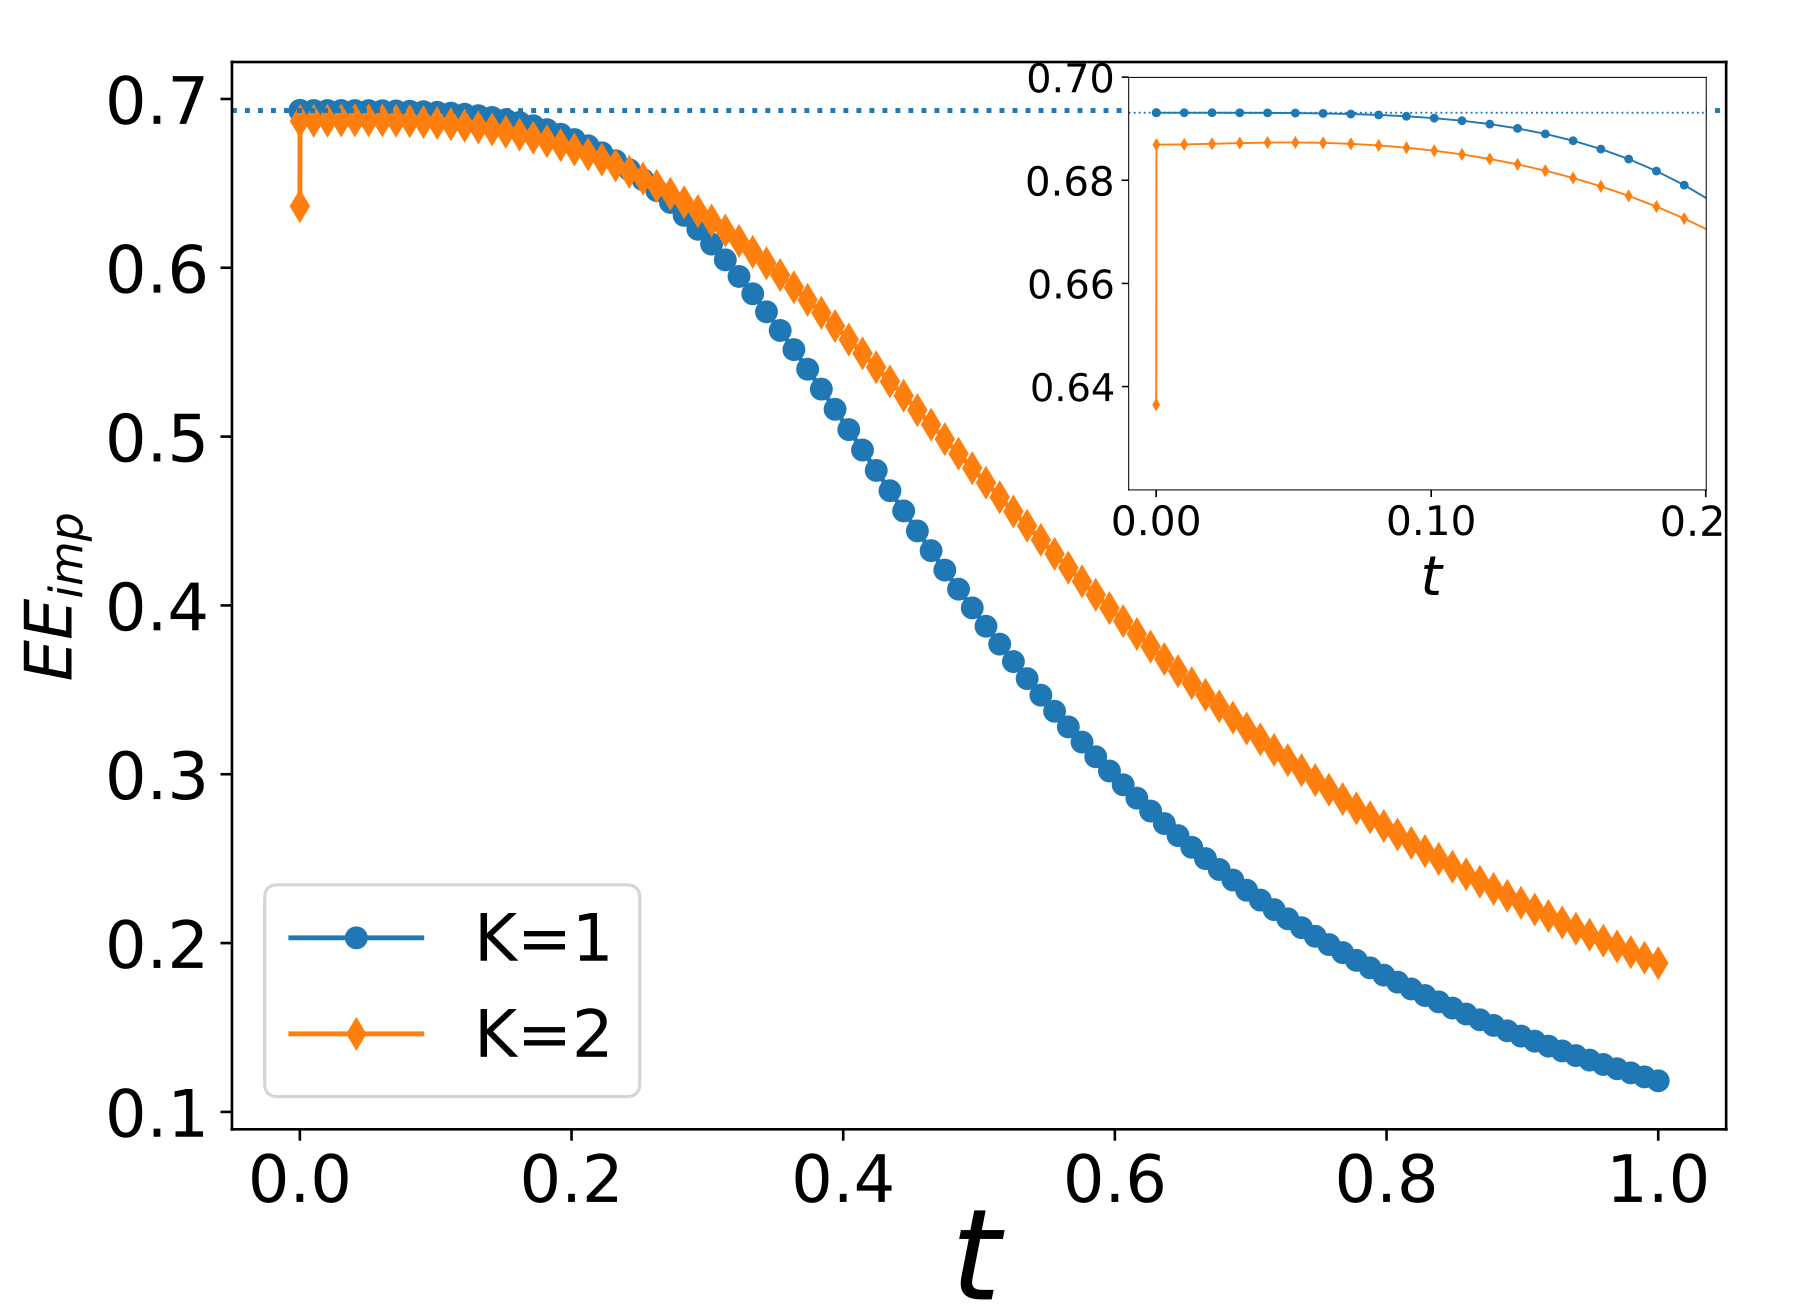
\includegraphics[scale=0.42]{plt/EE_imp_vs_t_K=12}
%\caption{This Figures shown the variation of impurity entanglement entropy $EE_{imp}$ with the variation of the hopping strangth $t$ for three different channel cases, $K=1,2,3$. In this case we have fixed $\alpha=1$.}
%\label{fig:EE_imp_vs_t_K}
%\end{figure}
%
%\subsubsection{Impurity entanglement entropy}
%\noindent  First, we are interested in the impurity entanglement entropy which is a measure of entanglement of the impurity with the rest. To do so we calculate the ground state of the Hamiltonian Eq.\eqref{eq:excitation_hamiltonian} $|\psi_g(t)\rangle$ followed by density matrix $\rho_g(t)=|\psi_g(t)\rangle \langle\psi_g (t)|$. Then we calculate the reduced density matrix by partial tracing the impurity $\rho_{imp}(t)=Tr_{imp} \rho_g(t)$. By diagonalizing the reduced density matrix $\rho_{imp}(t)$ we get the eigenvalues $\lambda_i(t)$ and the von-Neumann entanglement entropy $EE_{imp}(t)=-\sum_i\lambda_i(t) \log \lambda_i(t)$. As shown in the Fig.\ref{fig:EE_imp_vs_t_K} for all the three channel cases at low hopping strength $t$ there is a plateau in the $EE_{imp}$ measurement before it starts to decline with the further increase of hopping strength. At low $t\ll 1$ single channel has the higher impurity entanglement, which decreases by the increase of the channel number. On the other hand at high hopping strength value we see a different ordering of the impurity entanglement entropy. Higher the channel number slower the fall of the $EE_{imp}$ with the increase of $t$. This shows that, multiple channels protects the impurity better in terms of impurity  entanglement entropy making the multi channel problem more robust against the single channel case. 
%\par Though the plateau value of the impurity entanglement entropy at low hopping strength is very close to each other for different channel cases, there is a distinct difference between them. For the single channel case, the impurity entanglement entropy varies smoothly with the increase of $t$ from zero to nonzero value without any discontinuity. On the other hand for higher channels like $K=2$ and $K=3$ there is a discontinuity in the impurity entanglement entropy at $t=0^+$.
%
%
%\begin{figure}[!h]
%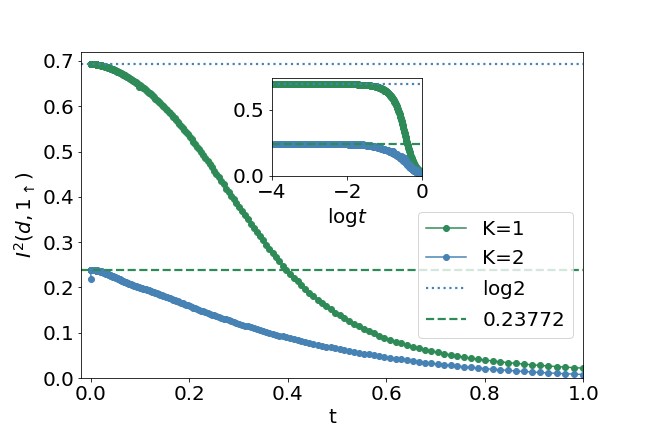
\includegraphics[scale=0.40]{plt/A_I2_ch12_['d','1_up']}
%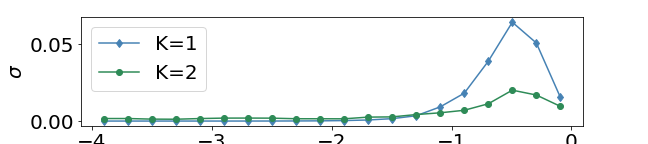
\includegraphics[scale=0.40]{plt/errorbar_A_I2_ch12_['d','1_up']}
%\caption{This figure show the variation of mutual information between the impurity spin and $1_{\uparrow}$ state with respect to the variation of the hopping strength $t$. For more details please refer to the text. In the figure above $\gamma=0.2195$.}
%\label{fig:MI_imp_1_vs_t_K}
%\end{figure}
%
%\subsubsection{Intra-channel Mutual information}
%
%\noindent Here we are interested in calculating Mutual information between two Fock states in the ground state wavefunction as a function of the hopping strength $t$ varying from $0$ to non zero values. Mutual information between two sub-systems $A,B$ is defined as $MI(A:B)=S(A)+S(B)-S(A\cup B)$, where $S(A)$ is the von-Neumann entanglement entropy of the sub-system $A$ with the rest of the system. 
%
%\noindent To find out the entanglement present between two Fock states within a single channel, we calulate the intra-channel mutual information.
%
%\par \textit{Case 1:} First, we study the mutual information between the impurity spin $S_d$ and $1_\uparrow$ Fock state (Fig.\ref{fig:schematic_hopping}) represented as $MI(d,1\uparrow)$, where $1$ is realspace origin of the $1^{st}$ conduction channel. For single channel case this $1_{\uparrow}$ site can be chosen uniquely but for $K$ channel cases there are $K$ possible choices, due to the symmetry any one choice will show similar mutual information signature. Similarly due to the $SU(2)$ spin rotation symmetry the mutual information between the impurity spin and $1_{\downarrow}$ state will not be any different. We have numerically computed the variation of mutual inforamtion with respect to the hopping strength $t$ and presented in the Fig.\ref{fig:MI_imp_1_vs_t_K}.  As shown in the inset of the Fig.\ref{fig:MI_imp_1_vs_t_K} at low hopping strength the mutual information for both the single channel and twochannel cases is saturating at different values. In the single channel case the Mutual information for $t=0$ is $MI(d,1_{\uparrow})=\log 2$ and changes smoothly to nozero $t$ values, similar to the previous impurity entanglement entropy study ($EE_{imp}$).
%\begin{eqnarray}
%S_{d}=S_{1_{\uparrow}}=S_{d,1_{\uparrow}}=\log 2~,~MI(d,1_{\uparrow})=\log 2
%\end{eqnarray}
%This $\log 2$ value shows the stability of the zero mode of single channel and perfect screening. Next we focus to the two channel case where the mutual information is $MI(d,1_{\uparrow})=0.2401$ which is less than the single channel case showing the breakdown of screening. Note, unlike the single channel case there is a discontinuity in $MI(d,1_{\uparrow})$ at $t=0^+$.
%
%
%
%\begin{figure}[!h]
%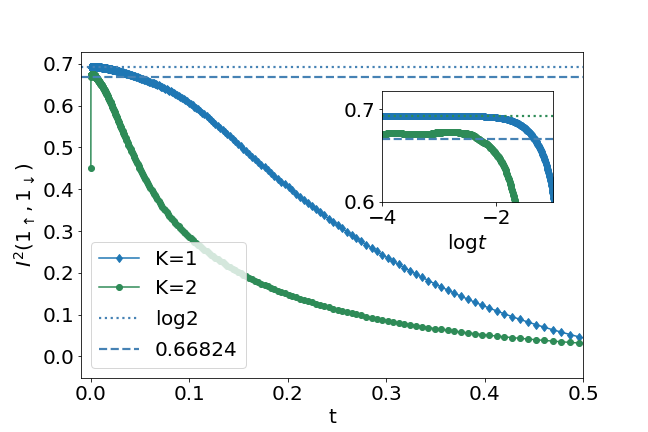
\includegraphics[scale=0.4]{plt/A_I2_ch12_['1_up','1_down']}
%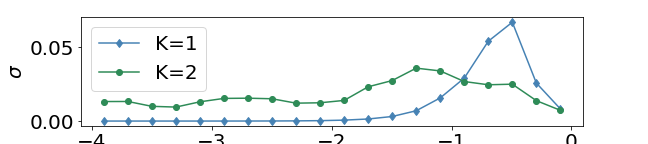
\includegraphics[scale=0.4]{plt/errorbar_A_I2_ch12_['1_up','1_down']}
%
%\caption{This figure shows the variation of mutual information among the two fock states present on the realspace origin of a conduction channel with $t$. In the figure above $\delta=0.450$}
%\label{fig:MI_1_2_vs_t_K}
%\end{figure}
%
%\par\textit{Case 2:} Similarly we have computed the mutual information $MI(1_{\uparrow},1_{\downarrow})$ (Fig.\ref{fig:MI_1_2_vs_t_K}) which measures intra channel  mutual information beteen two fock states $1_{\uparrow},1_{\downarrow}$ present at realspace origin. We find that the Mutual information is a smooth function of $t$ for single channel and for two channel there is a discontinuity at $t=0^{+}$. Note, $MI(1_{\uparrow},1_{\downarrow})>MI(d,1_{\uparrow})$ for all $t$ values show the presence of stronger intra-site correlation.
%
%\begin{figure}
%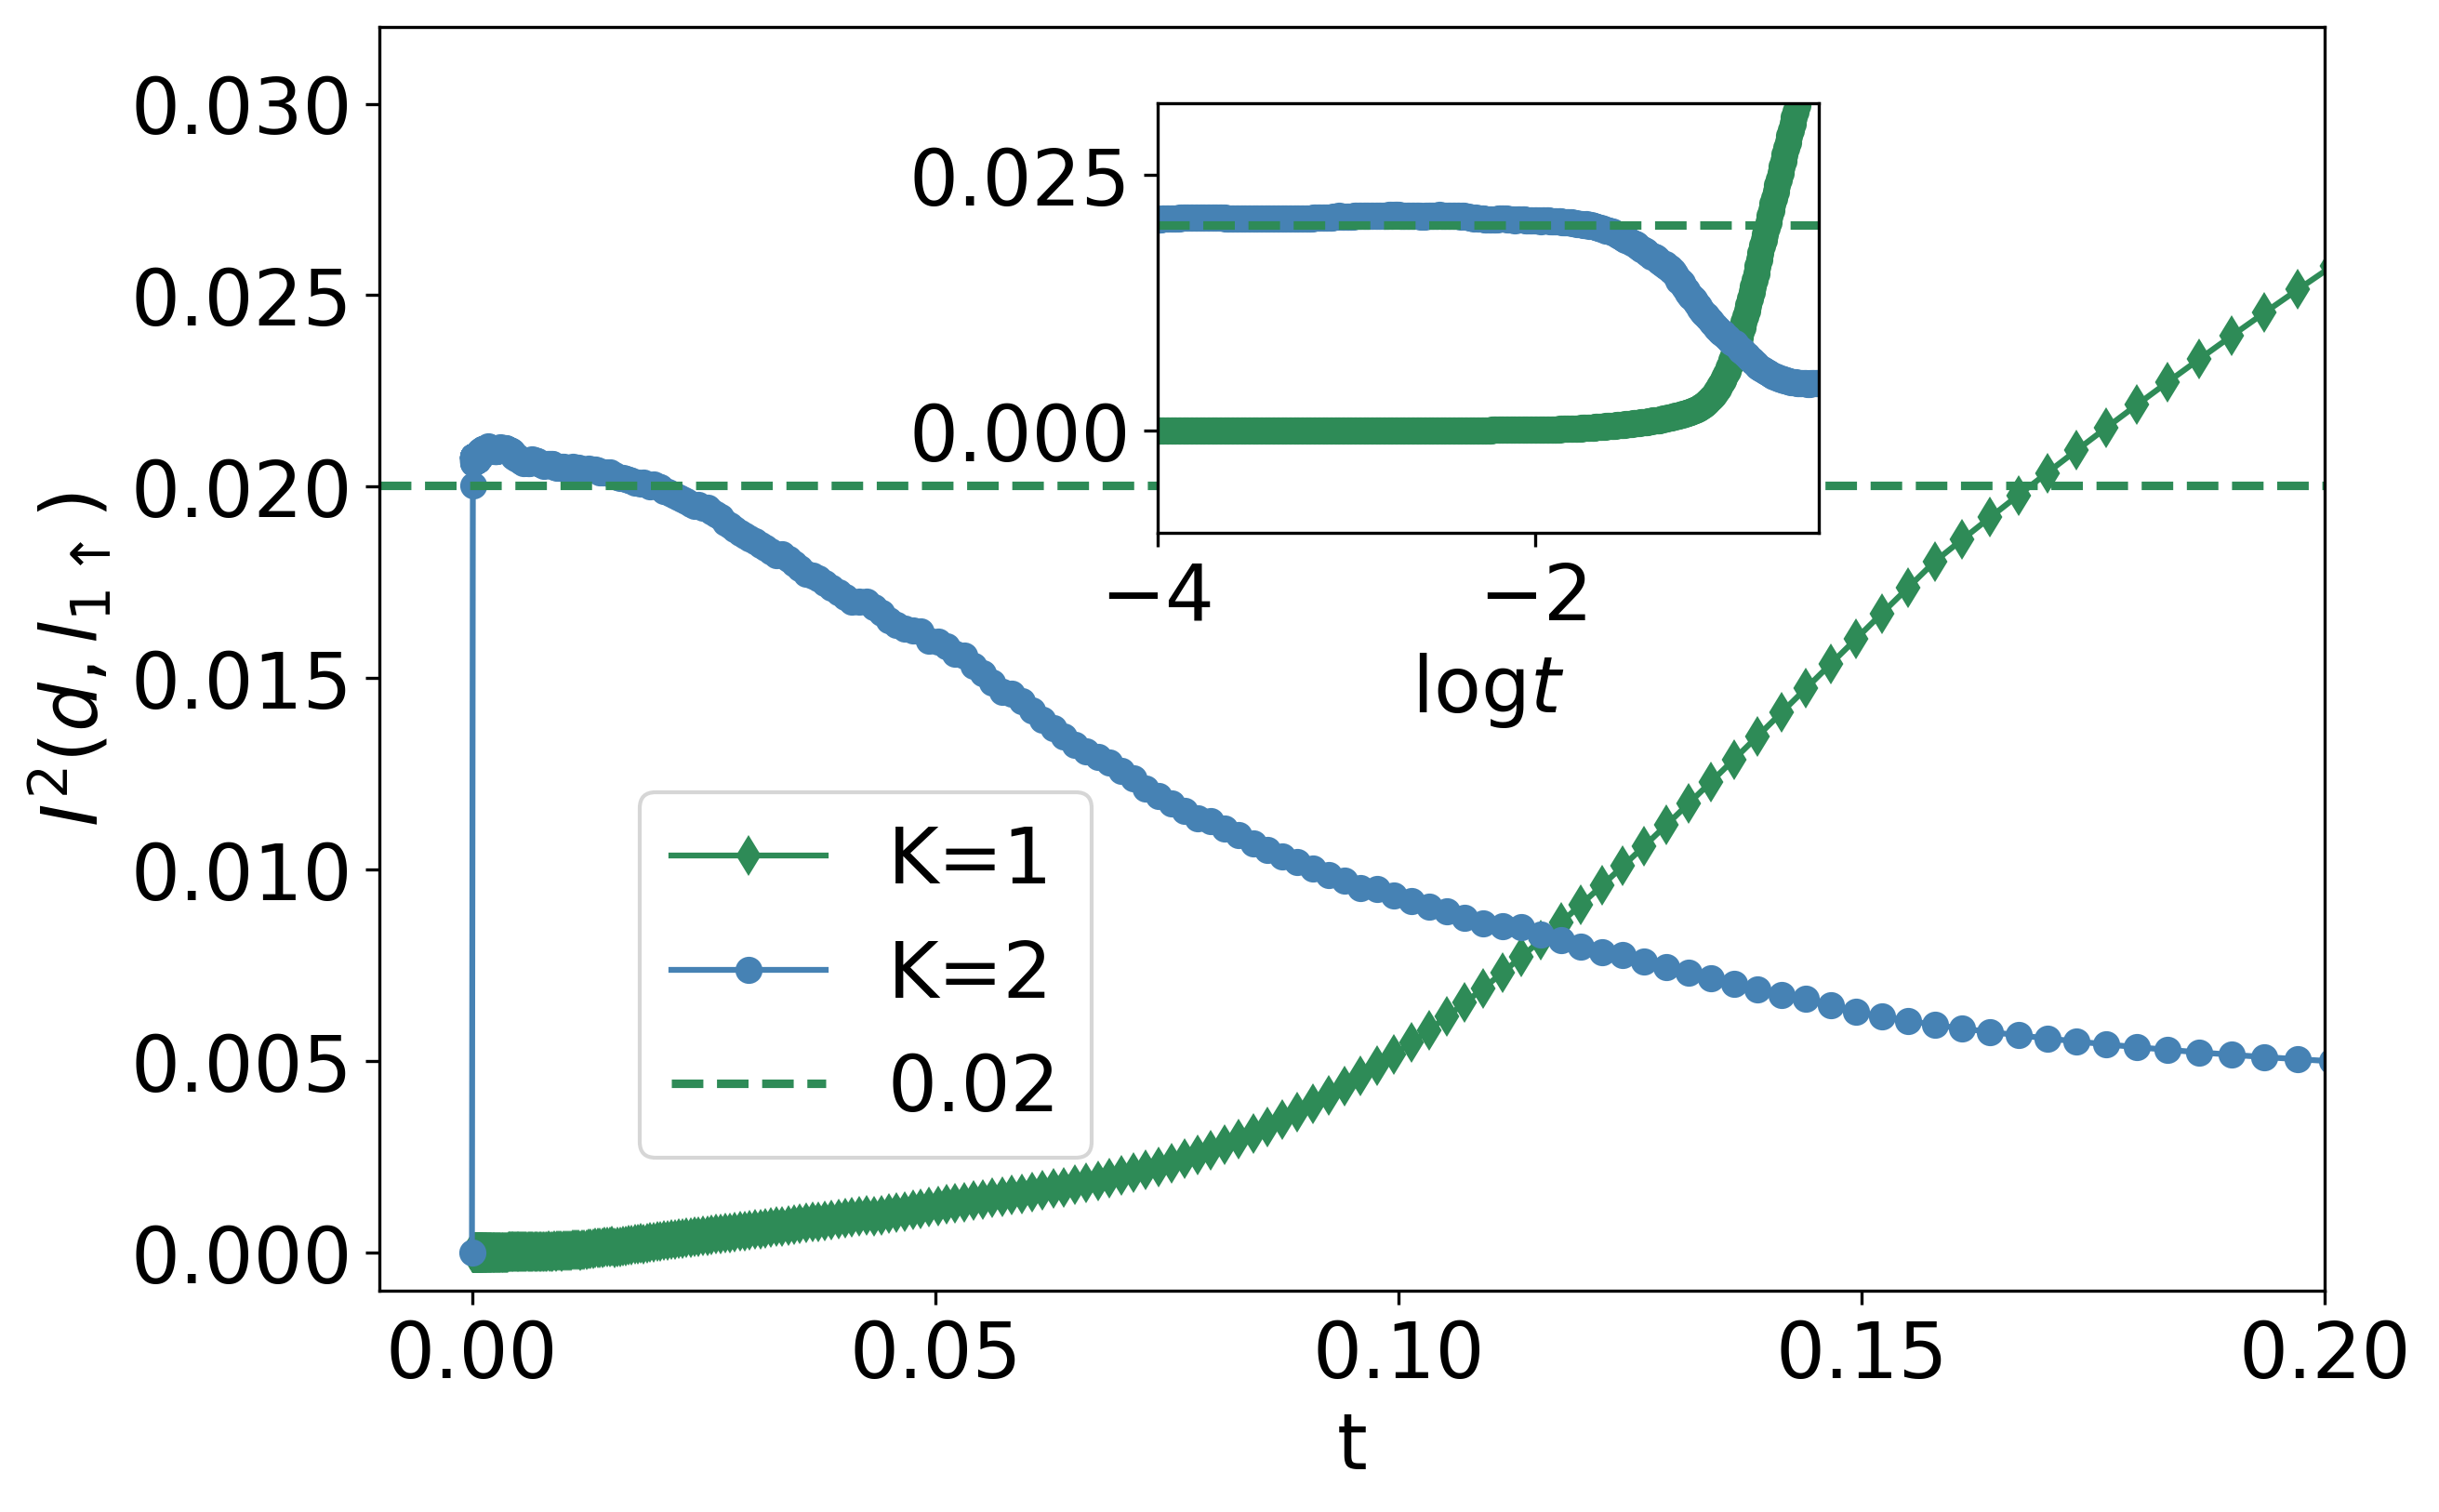
\includegraphics[scale=0.4]{plt/A_I2_ch12_['d','l1_up']}
%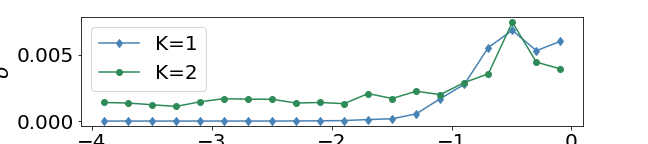
\includegraphics[scale=0.4]{plt/errorbar_A_I2_ch12_['d','l1_up']}
%\caption{$MI(d,l_{1\uparrow})$}
%\label{fig:MI_d_l1}
%\end{figure}
%\par \textit{Case 3:} Here we measure mutual information between the impurity and the Fock state of the nearest neighbor site to the realspace origin (Fig.\ref{fig:schematic_hopping}) of the conduction channel, $MI(d,l_{1\uparrow})$ as shown in the Fig.\ref{fig:MI_d_l1}. Vanishing mutual information for the single channel case shows the perfect screening of the impurity spin. On the other had we expect the breakdown of screening in two channel case, which is confirmed by the non-zero value of mutual information at small $t$ values. Here also we find a dicontinuity inthe mutual information at $t=0^+$.
%
%
%\begin{figure}[!h]
%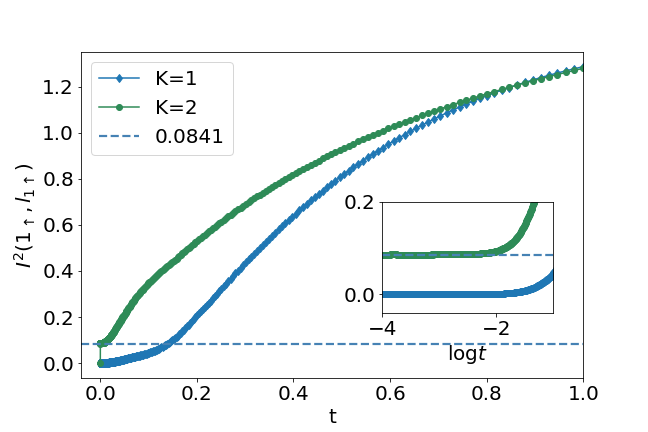
\includegraphics[scale=0.4]{plt/A_I2_ch12_['1','l1']}
%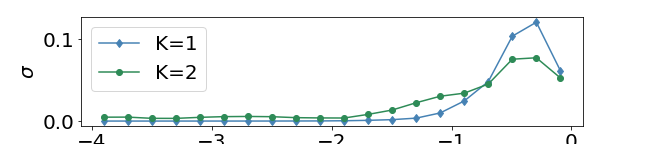
\includegraphics[scale=0.4]{plt/errorbar_A_I2_ch12_['1','l1']}
%\caption{$MI(1_{\sigma},l_{1\sigma})$}
%\label{fig:MI_l_l1}
%\end{figure}
%
%\par \textit{Case 4:} Another complementary study can be made by measuring the mutual information between conduction channel realspace origin and it's nearest neighbor site to check their mutual entanglement. As shown in the Fig.\ref{fig:MI_l_l1}, we find that at low hopping strength the single channel mutual information vanishes showing the decoupling of those two states. On the other hand in the two channel case there is a nonzero mutual information which verifies the presence of active scattering between the local Mott liquid and the local non-Fermi liquid phases. Similar discontinuity in the mutual information was observed at $t=0^+$.
%
%
%\par All the above  entanglement studies suggest that for two channel problem there is a discontinuity in the ground state at $t=0^{+}$, whereas for the single channel case it is a smooth function. Thus for single channel case the $t=0$ and $t\neq 0$ cases can be adiabtically connected, which is not the case for any other channel cases. 
%
%
%\subsubsection{Inter-channel Mutual information}
%Apart from the intra-channel mutual information, here we study the mutual information between two channels to calculate the entanglement content within the local Mott liquid phase.
%\begin{figure}
%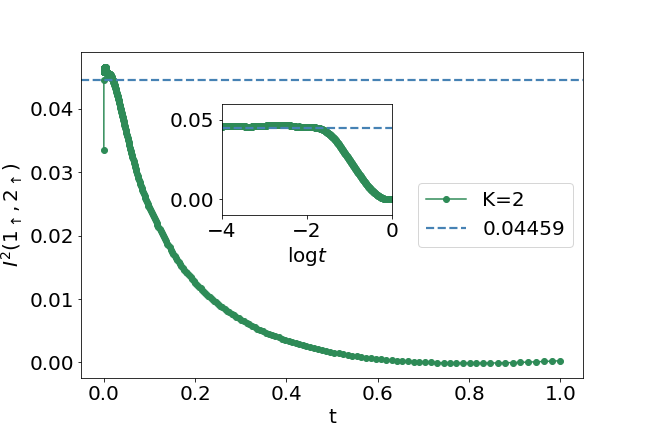
\includegraphics[scale=0.4]{plt/A_I2_ch2_[1,3]}
%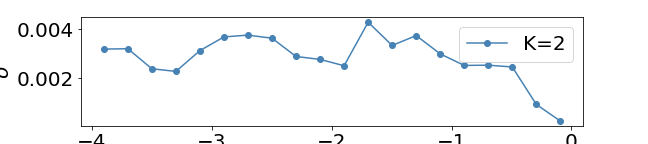
\includegraphics[scale=0.4]{plt/errorbar_A_I2_ch2_[1,3]}
%\caption{$MI(1_{\sigma},2_{\sigma'})$}
%\label{fig:MI_1_2}
%\end{figure}
%In the Fig.\ref{fig:MI_1_2} above we study the mutual information $MI(1_{\sigma},1_{\sigma'})$ between two Fock states $1_{\sigma},1_{\sigma'}$ as shown in the Fig.\ref{fig:schematic_hopping} for the two channel case. This shows that at low hopping strength there is a non-zero mutual information. This confirms the presence of correlation among channels. Apart from mutual information we have also computed the tripartite information across channels for this two channel case in the presence of non-zero hopping.
%\subsubsection{Tripartite information}
%
%\begin{figure}
%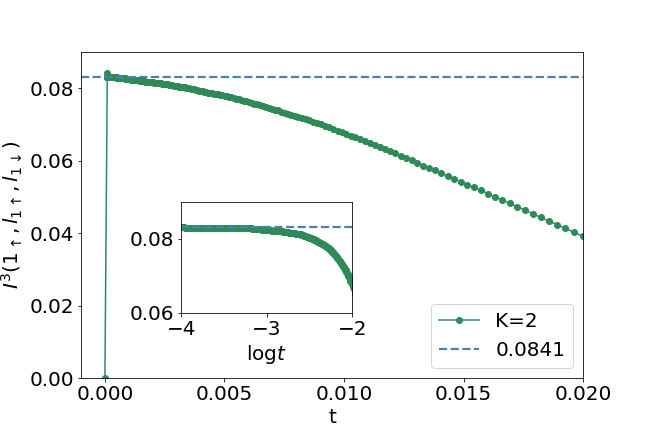
\includegraphics[scale=0.4]{plt/A_I3_ch2_[1,5,6]}
%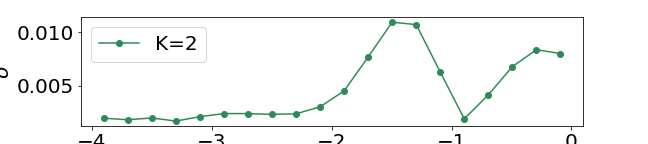
\includegraphics[scale=0.4]{plt/errorbar_A_I3_ch2_[1,5,6]}
%\caption{Tripartite information TPI 156}
%\label{fig:TPI_1_5_6}
%\end{figure}
%As shown in the result above Fig.\ref{fig:TPI_1_5_6} the tripartite information has a discontinuity at $t=0^+$. For small $t$ values the presnece of non-zero tripartite information signals the presence of tripartie correltaion in the ground state which agrees with presence of Marginal Fermi liquid phase shown by the effective Hamiltonian study.
%
%
%\subsubsection{Bures distance and orthogonality catathrope}
%\noindent Apart from different entanglement measures we have measured the Bures distance, which is a measure of distance between two density matrices. Which is defined as 
%\begin{eqnarray}
%d_{Bures}(\rho_1,\rho_2) &=& \sqrt{2} \bigg[1- \textrm{Tr}\bigg\{ \bigg(\rho_1^{1/2}  \rho_2 \rho_{1}^{1/2}\bigg)^{1/2} \bigg\}\bigg]
%\end{eqnarray}
%One can see from the above defination that, the maximum and minimum distance it can have is $\sqrt{2}$ and $0$ respectively. This measure represents the distance between two states in a Hilbert space. 
%\par We get the ground state wavefunction of the problem by solving the Hamiltonian Eq.\eqref{eq:excitation_hamiltonian} $|\psi(t)\rangle$ which is a function of $t$ and $\rho(t)= |\psi(t)\rangle \langle \psi(t)|$. We are interested in the reduced density matrix of the stargraph sites, to get that we partial trace out all other nearest neighbor sites, $\rho_{sg}(t)=\textrm{Tr}_{NN}(\rho(t))$. Then the Bures distance between the reduced denisty matrices $\rho_{sg}(t=0)$ and $\rho_{sg}(t)$, denoted as $d_{Bures}(\rho_{sg}(t=0),\rho_{sg}(t))$ are computed for single, two and three channel cases.
%\begin{figure}[!h]
%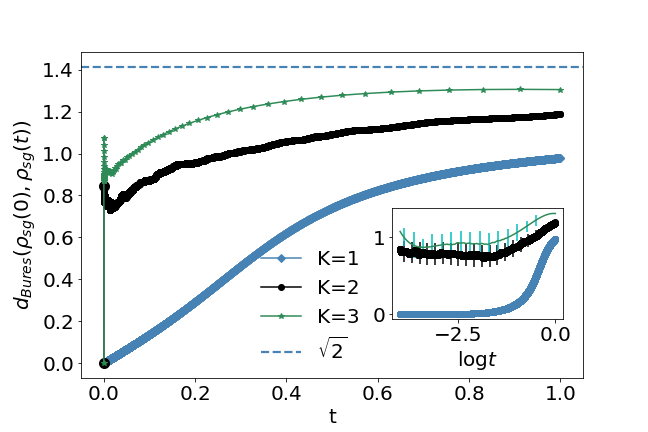
\includegraphics[scale=0.4]{plt/error_Bures_Distance_Ch123_10001}
%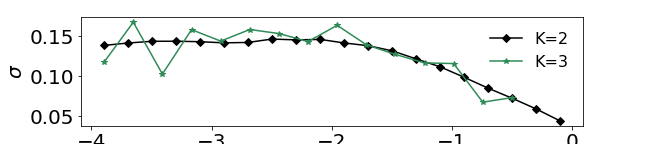
\includegraphics[scale=0.4]{plt/errorbar_Bures_Distance_Ch123_10001}
%\caption{Bures distance}
%\label{fig:bures_distance}
%\end{figure}
%We have shown the variation of the Bures distance as a function of the hopping strength in the Fig.\ref{fig:bures_distance} above. For all three cases the Bures distance is zero at $t=0$, whic is obvious. But as you turn on $t$ slightly there is a discontinuity in the distance for two and theree channel cases against the single channel where the distance varies smoothly. This discontinuity in the higher channel case against the single channel is similar to all the above entanglement studies. The smooth variation of the distance in the single channel case shows the adiabatic continuation of the reduced stargarph density matrix from the $t=0$ case to $t\neq 0$ case. On the other had the abrupt jump in the Bures distance for higher-channel cases at $t=0^+$ shows the breakdown of adiabatic continuity siganling an orthogonality catastrophe. Three channel case show higher amoount of discontinuity than the two channel case saturating at higher value for $t=1$. Due to finite size system we cannot see the exact orthogonality by getting the $d_{Bures}=\sqrt{2}$, but higher channel cases with higher discontinuity suggests so.
%
%
%
%
%
%
%
%
%
%
%
%
%
%\section{Strong-weak duality of the general spin-\(S\) impurity multi-channel Kondo model}
%We start from a strong coupling \((J \to \infty)\) spin-\(S\) impurity MCK Hamiltonian in the over-screened regime \(\left( K > 2S \right) \),
%\begin{equation}\begin{aligned}
%	\label{strong_ham}
%	H(J) = \sum_{k,\sigma,l}\epsilon_{k,l} \hat n_{k\sigma,l} + J \vec{S_d}\cdot\vec{s}_\text{tot}~.
%\end{aligned}\end{equation}
%Here, \(\vec s_\text{tot}\) is the total spin \(\sum_l \sum_{kk^\prime \alpha\beta} \vec \sigma_{\alpha\beta}c^\dagger_{k\alpha,l}c_{k^\prime\beta,l}\) of all the zero modes. At strong coupling, the ground states of the star graph eq.~\ref{stargraph} act as a good starting point for a perturbative expansion. As argued previously, there are \(K-2S+1\) ground states, labeled by the \(K\) values of the total spin angular momentum \(S^z = S_d^z + s_\text{tot}^z = -\frac{K}{2} + S, -\frac{K}{2} + S + 1, \ldots, \frac{K}{2} - S\). To leverage the large coupling, one can define a new spin impurity \(\mathbb{S}\) out of this ground state manifold. Since the degeneracy of a spin is given by its multiplicity \(2S^\prime + 1\), we have \(2S^\prime + 1 = K-2S+1 \implies S^\prime = \frac{K}{2} - S\). That is, the spin-\(S\) impurity has a dual described by a spin-\((K-2S+1)\) impurity. The states of this new spin are defined by
%\begin{gather}
%	\mathbb{S}_d^z \ket{S^z} = S^z \ket{S^z},\nonumber\\
%	\mathbb{S}_d^\pm \ket{S^z} = \sqrt{S^\prime\left( S^\prime + 1 \right) - S^z\left( S^z \pm 1\right)} \ket{S^z \pm 1}
%\end{gather}
%The excited states of the star graph can be used to define bosons \cite{kroha_kolf_2007}, and the hopping into the lattice can then be re-written using these Bosons. One can then remove the single-particle hoping between the zero modes and the first sites using a Schrieffer-Wolff transformation in the small coupling \(J^\prime = \gamma \frac{4t^2}{J}\), and generate an exchange-coupling between the new impurity \(\vec {\mathbb{S}}_d\) and the new zero modes formed out of the remaining sites in the lattice \cite{kroha_kolf_2007} (by remaining, we mean those real space sites that have not been consumed into forming the new spin). The new Hamiltonian, characterized by the small super-exchange  coupling \(J^\prime\), has the form
%\begin{equation}\begin{aligned}
%	H^\prime(J^\prime) = \sum_{k,\sigma,l}\epsilon_{k,l} \hat n_{k\sigma,l} + J^\prime \vec{\mathbb{S}_d}\cdot\vec{s^\prime}_\text{tot}
%\end{aligned}\end{equation}
%The prime on \(s_\text{tot}\) indicates that it is formed by the new zero modes. This Hamiltonian is very similar to the one in eq.~\ref{strong_ham}, and that is the essence of the strong-weak duality: One can go from the over-screened strong coupling spin-\(S\) MCK model to another over-screened weak coupling spin-\((K-2S+1)\) MCK model. For the case of \(K=4S\), we have \(S^\prime = S\), and both \(S_d\) and \(\mathbb{S}_d\) describe the same spin objects (at least formally). The two models are then said to be self-dual. For example, for the case of spin-half MCK model, two-channel model is self-dual.
%\begin{figure}[!htpb]
%	\centering
%	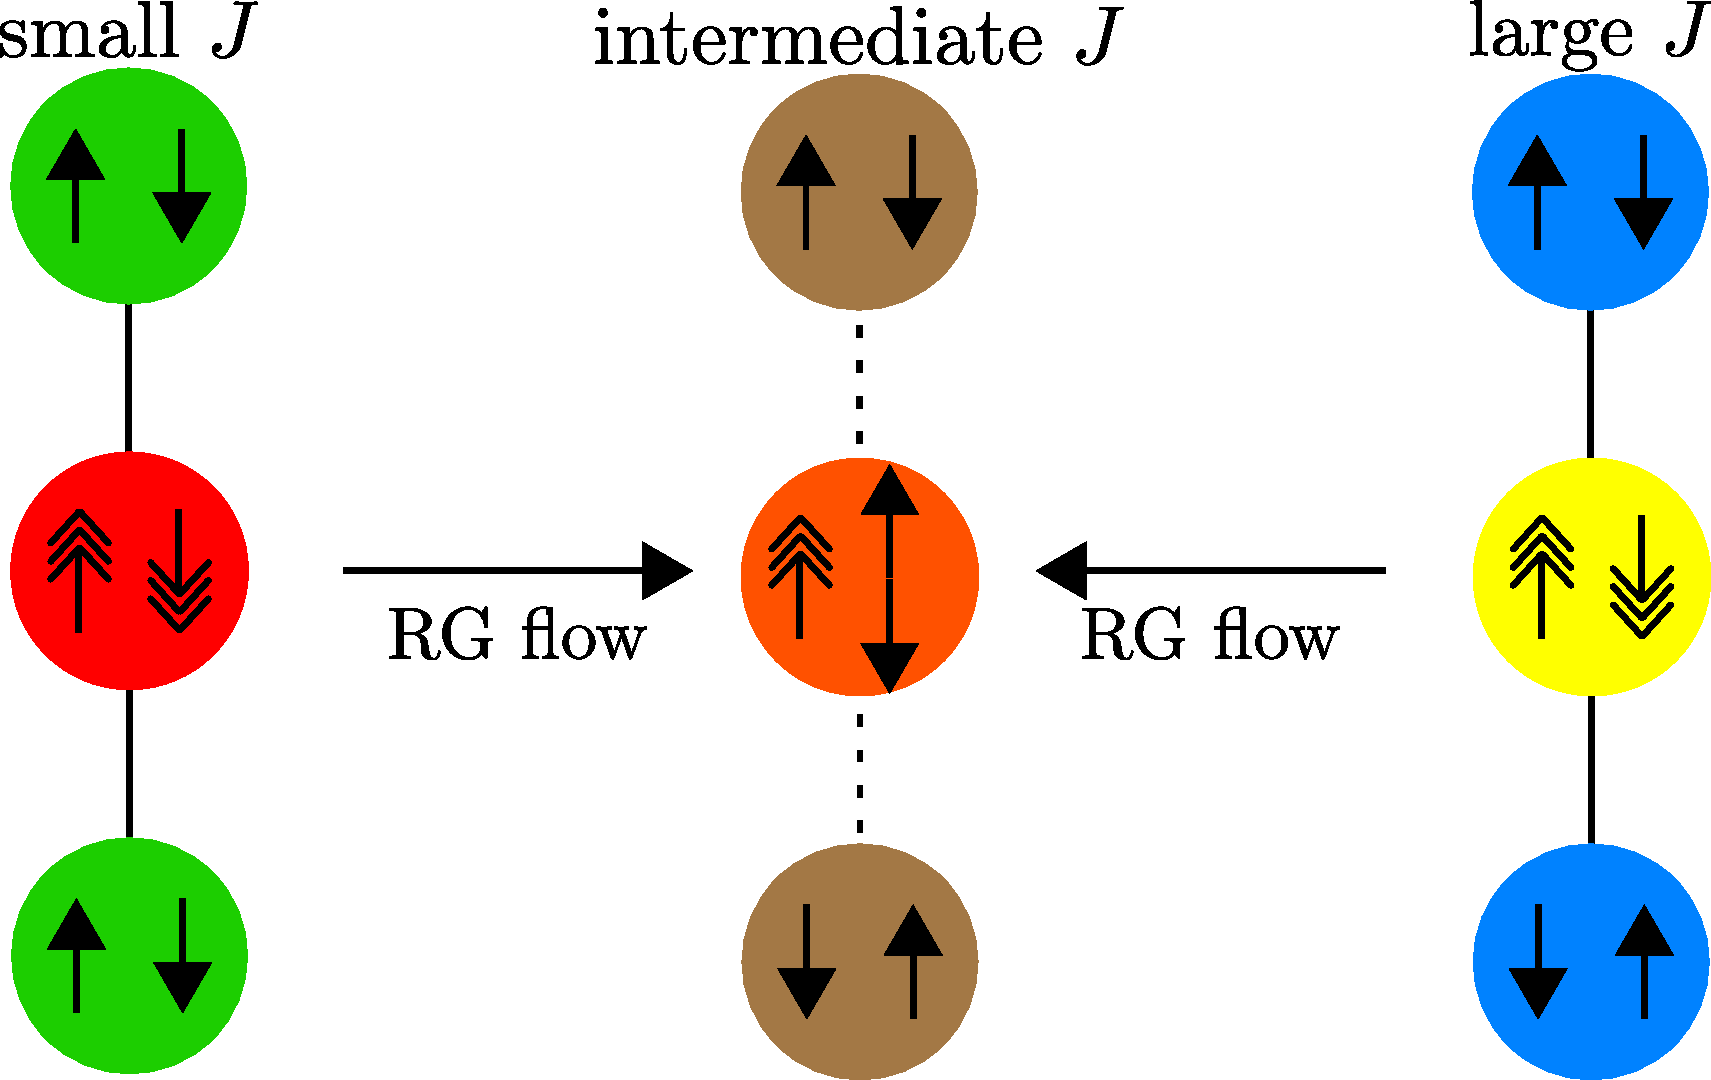
\includegraphics[width=0.3\textwidth]{plt/duality.pdf}
%	\caption{Duality of the RG flows as seen in the star graph Hamiltonian. The red and green circles represent the impurity and zeroth site spins respectively. At large \(J\), the red circle binds with the green circles to form an effective spin \(\frac{K-1}{2}\) object (yellow) that interacts with the remaining spin of the conduction bath (blue circles).}
%	\label{duality_fig}
%\end{figure}
%
%One important consequence of the duality relationship between the two over-screened models is that the RG equations are also dual; while the strong coupling model has an irrelevant coupling \(J\) that flows down to the intermediate fixed point \(J^*\), the weak coupling model has a relevant coupling \(J^\prime\) that flows up to the same fixed point \({J^\prime}^* = J^*\). From the RG equation for the general spin-\(S\) MCK model, we know that \({J^\prime}^* = \frac{2}{K \rho^\prime}\), where \(\rho^\prime\) is the DOS for the bath of the weak coupling Hamiltonian. This constrains the form of the scaling factor \(\gamma\):
%\begin{equation}\begin{aligned}
%	{J^\prime}^* = \frac{\gamma 4t^2}{J^*} = \frac{2}{K \rho^\prime} \implies \gamma = \frac{1}{4t^2} {J^*}^2 = \frac{1}{K^2 t^2 \rho \rho^\prime}
%\end{aligned}\end{equation}
%
%There exists another set of dual points in the MCK model. This was hinted at when we looked at the degree of compassion in eq.~\ref{gamma}. Since \(\Gamma\) depends only on the magnitude of \(\delta\), both \(\pm \delta\) will give the same degree of compensation, same ground state energy and same ground state degeneracy \(\left(g^S_K = |\delta|+1\right)\). The definition of \(\delta\) gives the duality transformation as \(K \to 2S, S \to \frac{K}{2}\). That is, we transform from a \(K-\)channel MCK model with spin-\(S\) impurity, to a \(2S\)-channel MCK with a spin-\(\frac{K}{2}\) impurity. The exactly-screened model \(K=2S\) maps on to itself and is therefore self-dual under this transformation.
%
%For \(K \neq 2S\), we transform an over-screened model into an under-screened model and vice versa. This duality relationship allows us to infer the RG scaling behaviour of one of the models if we know that of the other. If we know that for a certain pair of values \(K\) and \(S\), the \(K-\)channel MCK model with spin-\(S\) impurity has an intermediate fixed point, we can immediately conclude that the \(2S\)-channel spin-\(\frac{K}{2}\) model has a strong coupling fixed point.
%\begin{figure}[htpb]
%	\centering
%	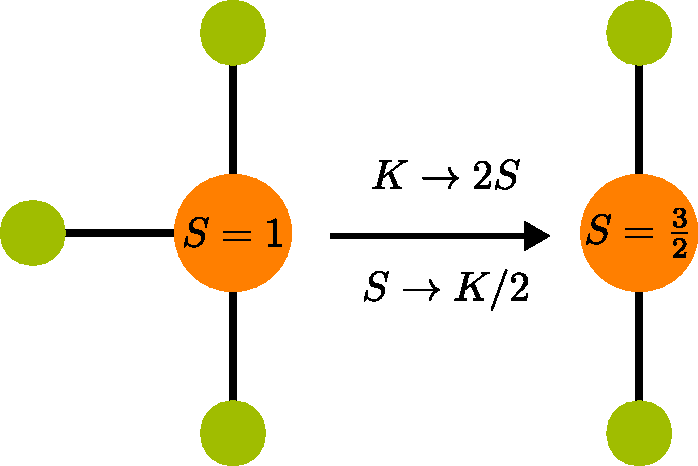
\includegraphics[width=0.3\textwidth]{plt/duality2.pdf}
%	\caption{./duality2.pdf}
%	\label{fig:-duality2-pdf}
%\end{figure}
%
%

%\section{Impurity Quantum Phase transition in the multi-channel Kondo model under channel anisotropy}
%\label{anisotropic_rg}
%\subsection{RG analysis}
%The isotropic MCK mode undergoes a phase transition when the symmetry of the channel interaction strengths is destroyed. We will now summarize the conclusions of this section. It will be shown analytically that if, in a \(K-\)channel model, one of the couplings becomes slightly larger than the other \(K-1\) couplings, the system goes into the singlet ground state characterized by local Fermi liquid excitations. On the other hand, if one of the couplings becomes slightly smaller than the rest, the system goes over to the \(K-1\) channel Kondo model. \textit{This shows that in the context of the general anisotropic MCK model, the symmetric model is highly unstable under slight anisotropy, and undergoes a phase transition into either the \(K-1\) channel NFL phase or into the single channel LFL phase.}
%\begin{figure}[!htpb]
%	\centering
%	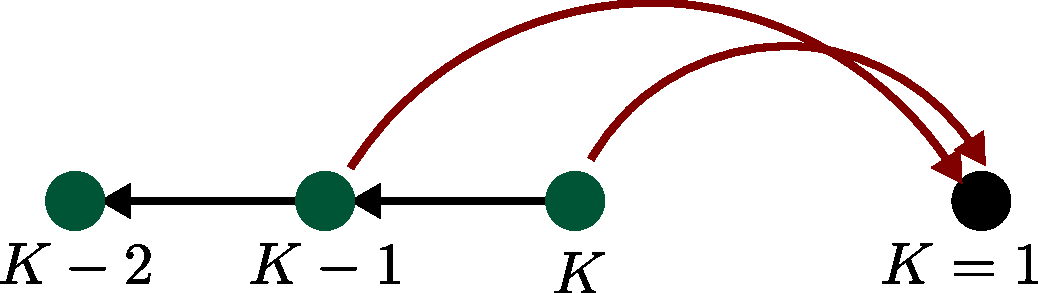
\includegraphics[width=0.3\textwidth]{plt/iqpt.pdf}
%	\caption{Transitions from one Kondo model to another under insertion of anisotropy. The green circles represents MCK models with \(K>1\) while the black circle represents the \(K=1\) model. The red lines indicate transition from the \(K\) channel MCK model to the single-channel model when one of the exchange couplings becomes larger than the others. The black lines indicate the transition from the \(K\) channel model to the \(K-1\) channel model when one of the exchange couplings becomes smaller than the others.}
%	\label{fig:-iqpt-pdf}
%\end{figure}
%
%To see the transition, we need to start with the more general anisotropic MCK model:
%\begin{align}
%	H = \sum_{k,\alpha,l}\epsilon_{k,l} \hat n_{k\alpha,l} + \sum_{kk^\prime,\atop{\alpha,\beta,l}}J_l \vec{S_d}\cdot\frac{1}{2}\vec{\sigma}_{\alpha\beta}c_{k\alpha,l}^\dagger c_{k^\prime\beta, l}~.
%\end{align}
%We now consider the specific case where \(K-1\) channels have the same coupling \(J_1 = J_2 = ... = J_{K-1} = J_+\) and the remaining channel has a different coupling \(J_K = J_-\). The RG equations for such a model are
%\begin{align}
%	\frac{\Delta J_\pm}{|\Delta D|} = -\frac{J_\pm^2 \rho}{\mathcal{D}_\pm} + \frac{\rho^2 J_\pm}{2}\left[\frac{(K-1)J_+^2}{\mathcal{D}_+} + \frac{J_-^2}{\mathcal{D}_-}\right]
%\end{align}
%where \(\mathcal{D}_\pm = \omega - \frac{D}{2} - \frac{J_\pm}{4}\) are the denominators of the URG equations.
%Setting \(J_+ = J_-\) leads to the critical fixed point at \(J_+^* = J_-^* = J_* = \frac{2}{K \rho}\). We now perturb around this fixed point by defining new variables \(j_\pm = J_\pm - J_*\). We also assume that the bandwidth is large enough so that \(\mathcal{D}_\pm \simeq \omega - \frac{D}{2} - \frac{J_*}{4} = -|\mathcal{D}_*|\). The RG equations then take the form
%\begin{widetext}
%\begin{align}
%	\frac{\Delta j_+}{|\Delta D|} &= \frac{\rho J_+}{ |\mathcal{D}_*|}\left[J_+ - \frac{\rho}{2}\left[(K-1)J_+^2 + J_-^2\right]\right] = \frac{\rho J_+}{K J_*|\mathcal{D}_*|}\left[-\left(K - 2\right)J_*j_+ - (K-1)j_+^2 - j_-^2 - 2J_* j_-\right]\\
%	\frac{\Delta j_-}{|\Delta D|} &= \frac{J_- \rho}{|\mathcal{D}_*|}\left[J_- - \frac{\rho}{2}\left[(K-1)J_+^2 + J_-^2\right]\right] = \frac{J_- \rho}{K J_*|\mathcal{D}_*|}\left[\left(K - 2\right)J_*j_-  - j_-^2 - (K-1)j_+^2 - 2(K-1)J_* j_+\right]\\
%\end{align}
%\end{widetext}
%We will first look at the special case of \(K=2\), the two channel Kondo model. The equations simplify to
%\begin{align}
%	\frac{\Delta j_\pm}{|\Delta D|} = \frac{J_\pm \rho}{K J_*|\mathcal{D}_*|}\left[- \left(j_+^2 + j_-^2\right) - 2J_* j_\mp\right]
%\end{align}
%For \(j_- < 0, j_+ > 0\), we have \(\Delta j_- < 0\). The coupling \(J_-\) therefore becomes irrelevant. For small \(j_+\), we have \(j_+^2 < 2J_* |j_-|\)  and \(\Delta j_+ > 0\). This means that the isotropic fixed point is repulsive under anisotropy~\cite{Noz_blandin_1980}. The coupling \(j_+\) being relevant means we have a single-channel Kondo problem. We already know the non-perturbative URG equation for the single-channel Kondo problem~\cite{kondo_urg}, and it leads to the strong coupling fixed point~\cite{Noz_blandin_1980,fabrizio_nozieres_1995,mitchell_bulla_2014}.
%
%We now look at the general \(K\) channel case. Let us first look at the regime \(j_- < 0, j_+ > 0\). In this regime, we have \(\Delta j_- < 0\), which means \(j_-\) will flow to larger negative values until it reaches \(j_- = -J_*\) such that \(J_- = J_* + j_- = 0\). \(j_+\) is, on the other hand, relevant for small values of \(j_\pm\). It will continue to grow until the numerator of \(\Delta j_+\) vanishes. This condition is given by
%\begin{align}
%	\left(K - 2\right)J_*j_+ + (K-1)j_+^2 + j_-^2 + 2J_* j_- = 0
%\end{align}
%Substituting \(j_- = -J_*\) gives the fixed-point equation \((K-1)j_+^2 + \left(K - 2\right)J_*j_+ - J_*^2 = 0\). Solving the equation gives
%\begin{align}
%	j_{+,*} = \frac{J_*}{2(K-1)}\left[-(K-2) \pm K\right] = \frac{J_*}{K-1}
%\end{align}
%At the final step, we chose the positive solution, because \(j_+\) is relevant in this regime. The new fixed point value of \(J_+\) is therefore
%\begin{align}
%	J_{+,*} = J_* + \frac{J_*}{K-1} = \frac{\frac{2}{K \rho} K}{K - 1} = \frac{2}{(K-1)\rho}
%\end{align}
%In other words, the \(K\) channel fixed point flows to the \(K-1\) channel fixed point. This is shown numerically in the left panel of fig.~\ref{K_to_K-1}.\\
%
%
%\begin{figure*}[!htpb]
%	\centering
%	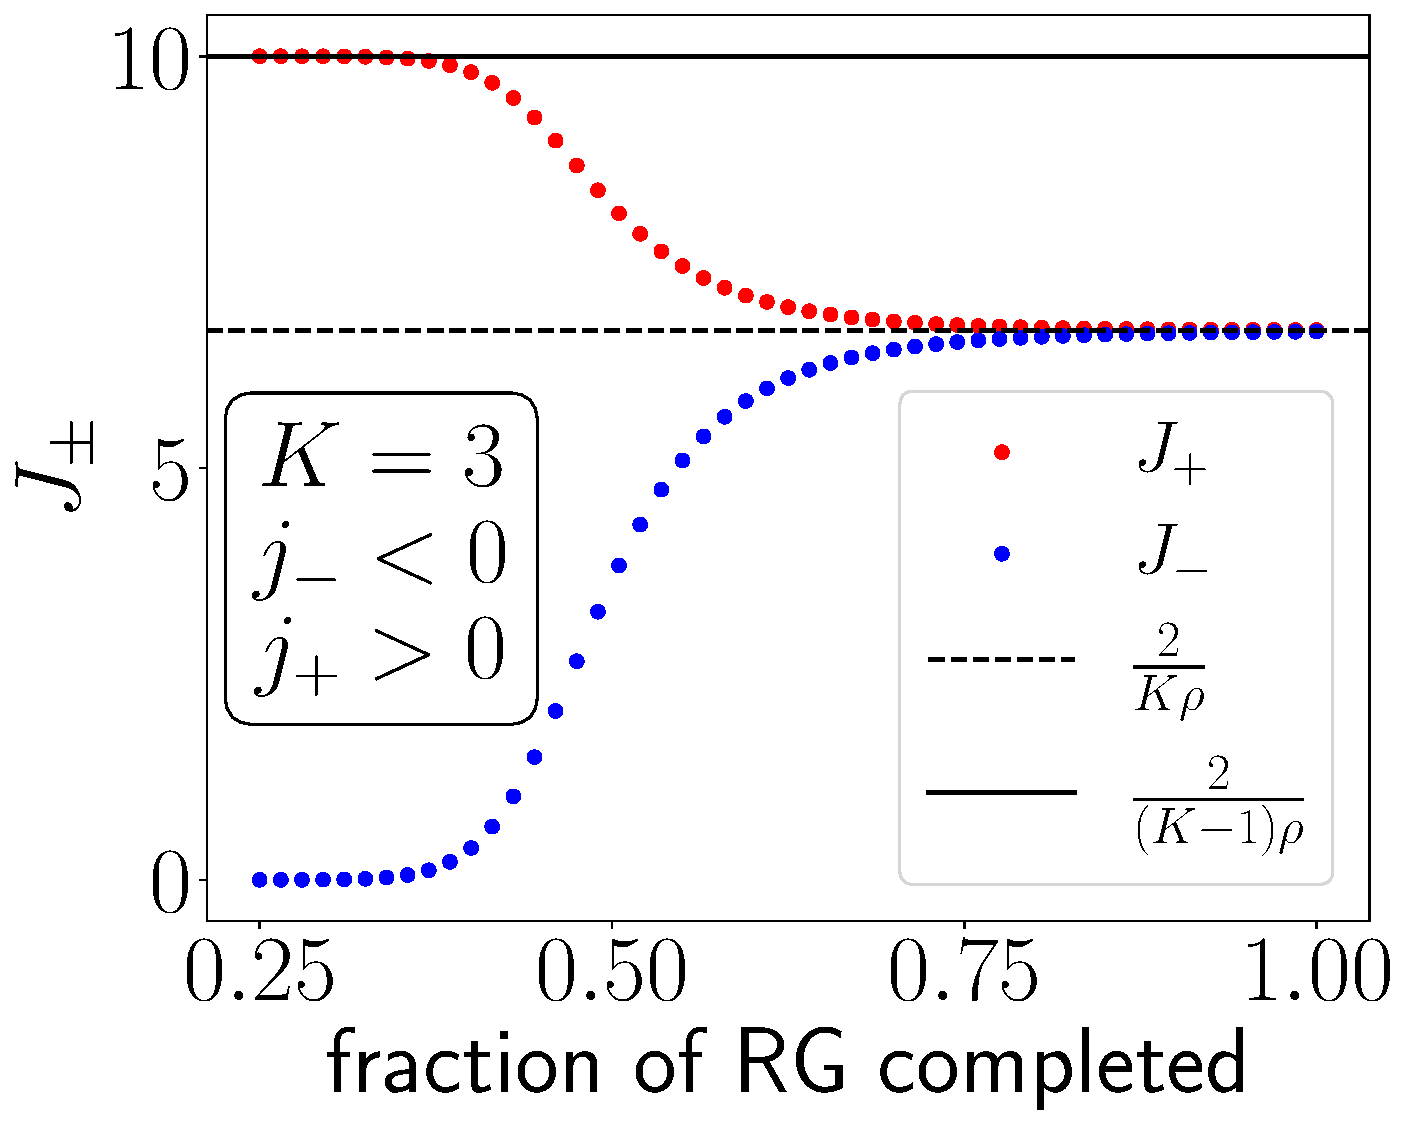
\includegraphics[width=0.3\textwidth]{plt/K to K-1.pdf}
%	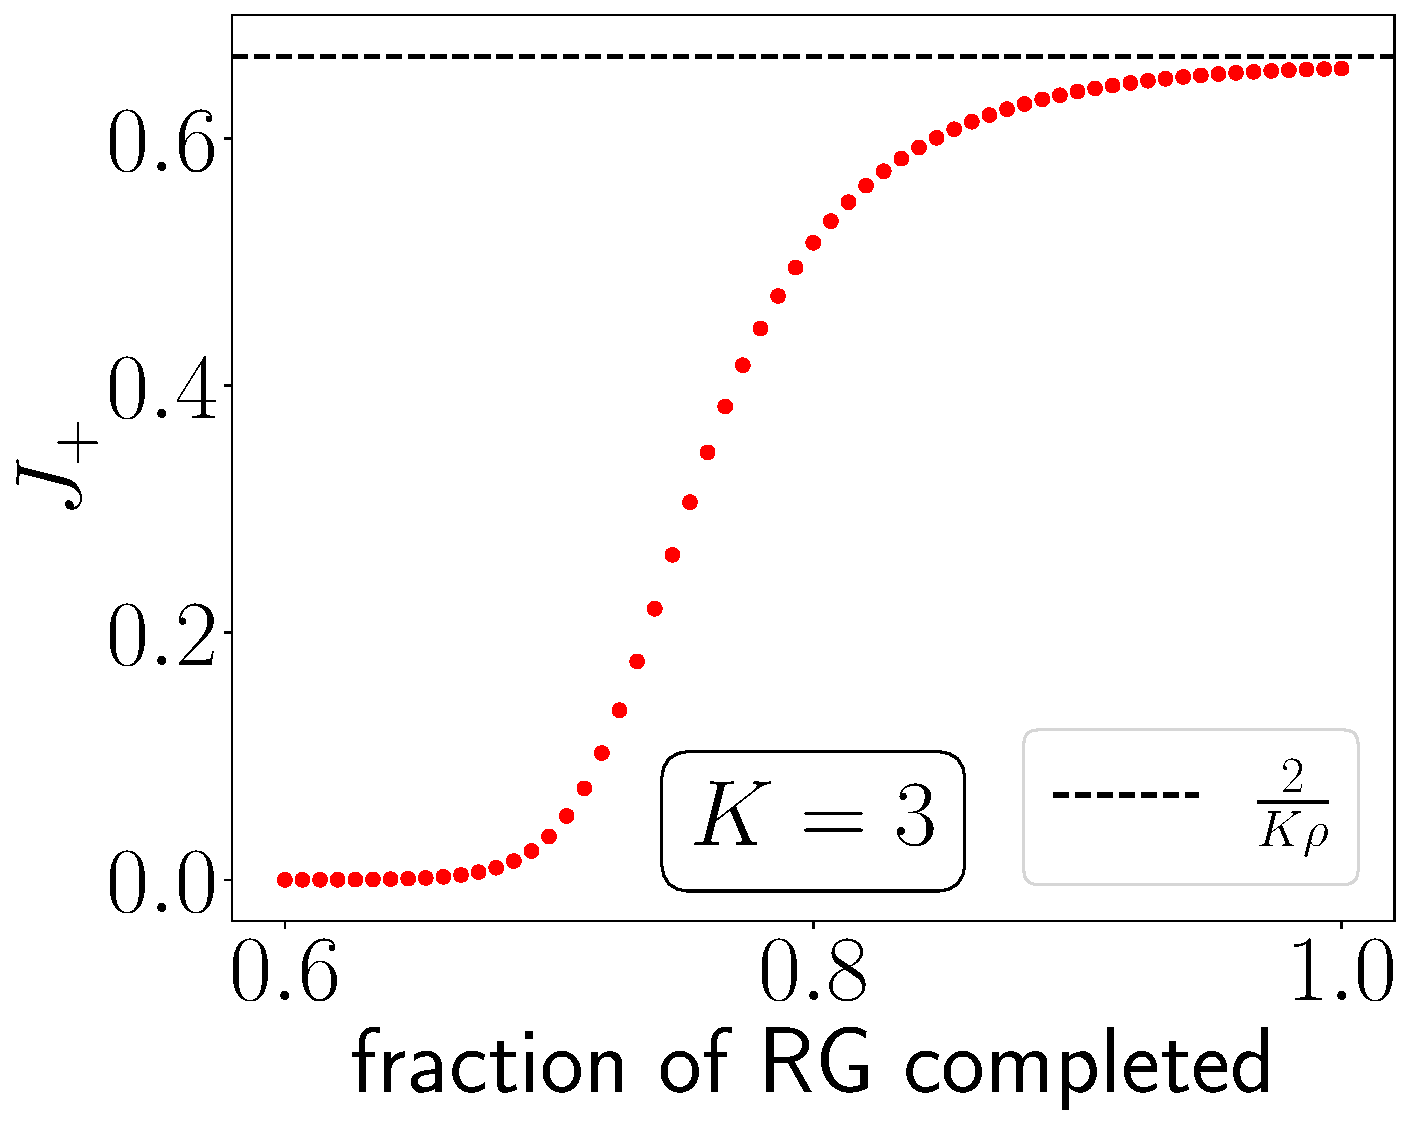
\includegraphics[width=0.3\textwidth]{plt/irr_Jp_K=3.pdf}
%	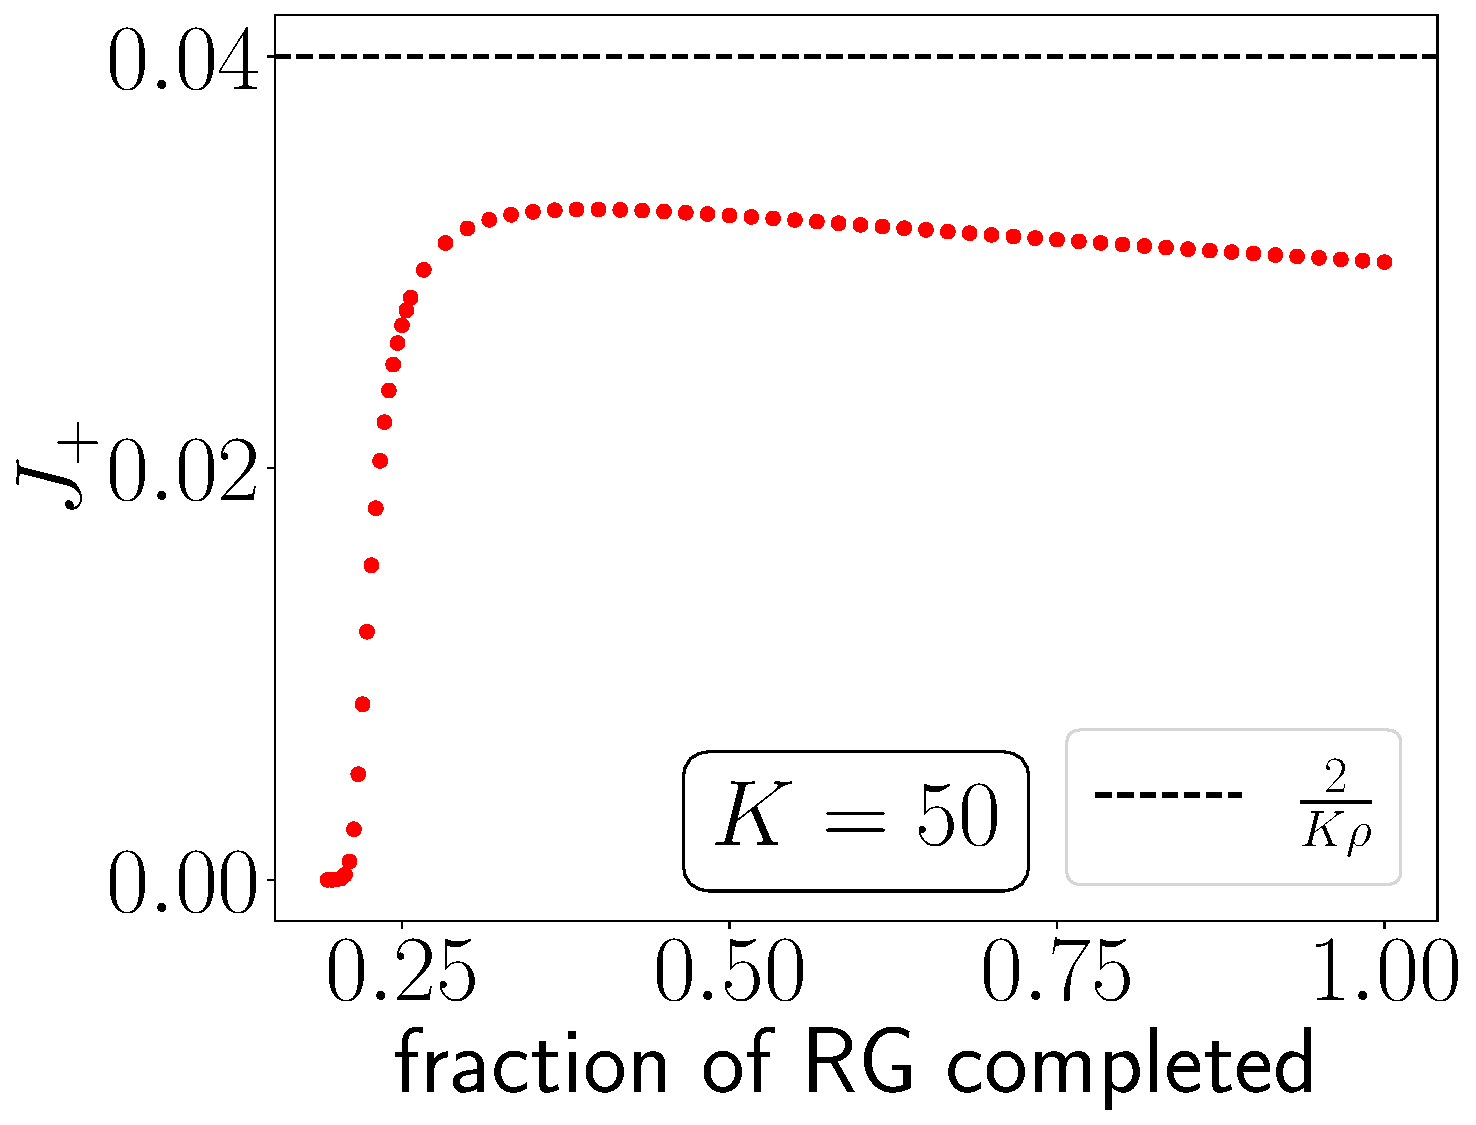
\includegraphics[width=0.3\textwidth]{plt/irr_Jp_K=50.pdf}
%	\caption{left panel: Flow of \(J_\pm\) when \(j_< 0\) and \(J_+\). The smaller coupling \(J_-\) is irrelevant and switches off, while the other \(K-1\) couplings \(J_+\) flow to the \(K-1\) MCK fixed point. Middle and right panels: Flow of the couplings \(J_+\) when \(j_+ < 0\) when \(j_- > 0, j_+ < 0\), for two values of \(K\). In both cases, the smaller coupling \(J_+\) eventually dies out, leading to only one surviving coupling \(J^-\) which is relevant, and we are left with a single-channel Kondo model.}
%	\label{K_to_K-1}
%\end{figure*}
%
%In the opposite regime \(j_- > 0, j_+ < 0\), \(\Delta j_+\) is negative. It has been checked numerically that \(J_+\) ultimately flows to zero in this regime (middle and right panels of fig. \ref{K_to_K-1}), and \(J_-\) remains relevant. Since there is no numerator fixed point in the relevant coupling \(J_-\) and because all other couplings are irrelevant, the equation for \(J_-\) is replaced by the single-channel Kondo coupling URG equation, and the low-energy physics is then of strong coupling.
%
%
%\subsection{Channel anisotropy}
%
%\noindent So far we have talked the stargraph problem where all the outer spin is coupled with the central impurity spin with Heisenberg cuopling of equal strength. This model has a special symmetry where any rearrangement of the outer spins keeps the stargraph Hamiltonian invariant. Here we wish to break this symmetry of this Hamiltonian by choosing the individual coupling strength of the outer spin with the central impurity spin different. We start with the general coupling Hamiltonian written as 
%\begin{eqnarray}
%H_K (\vec{\lambda}) &=& \sum_{i=1}^{K} \lambda_i\vec{S}_d.\vec{S}_i
%\label{eq:anisotropy}
%\end{eqnarray}
%
%\begin{figure}\centering
%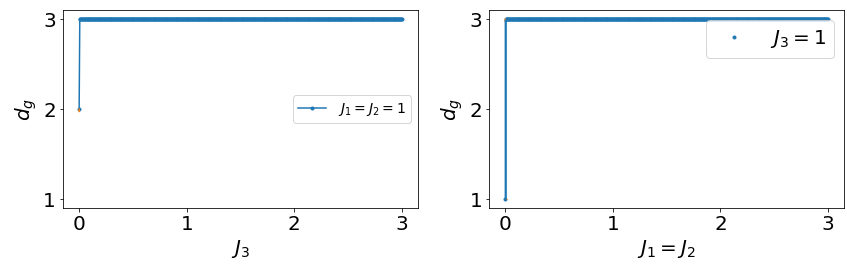
\includegraphics[scale=0.28]{plt/Anisotropy_Channel_3.png}
%\caption{channel anisotropy}
%\label{fig:channel-anisotropy}
%\end{figure}
%
%where $ \vec{\lambda} \equiv (\lambda_1,\cdots,\lambda_K)$ and $\lambda_i>0, \forall i$. So far we have considered the case where $\lambda_i=\alpha,~\forall i$. Numerical study of the Hamiltonian Eq.\eqref{eq:anisotropy} shown that for any values of couplig $\lambda_i>0$ the ground state degenracy for a $S_d=1/2$ is always $K$ fold, where $K$ is the number of channels. This shows the robustness of the ground state degeneracy of the stargraph model against the couling anisotropy. The ground state degeneracy only changes when atleast one coupling vanishes or becomes infinite. In the case when one coupling of $K$ channel anisotropic stargraph model vanishes, the effective model becomes a $K-1$ channel anisotropic stargraph model with $K-1$ fold degenrate ground states. On the other hand, if one of the $K$ couplings becomes infinite then with respect to that coupling other couplings becomes zero thus giving rise to an effective single channel stargraph model. For example, for $\lambda_K\rightarrow 0$, the Hamiltonian becomes $H_{K}(\vec{\lambda})\rightarrow H_{K-1}(\lambda_1,\cdots,\lambda_{K-1})$ and for $\lambda_K\rightarrow \infty$ we get $H_{K}(\vec{\lambda}) \rightarrow H_{1}(\lambda_K)$. 
%
%We have demonstrated this numerically for a three channel anisotropic stargraph model. As shown in the Fig.\ref{fig:channel-anisotropy}(a) where two couplings are same ($\lambda_1=\lambda_2=1$) and we are numerically varying the third coupling $\lambda_3$ from finite to zero. The degeneracy is alywas $3$ except when $\lambda_3=0$, then the degeneracy becomes $2$ becoming an effecive two channel problem. On the other hand in Fig.\ref{fig:channel-anisotropy}(b) we keep the first coupling $\lambda_3$ fixed to $1$ and vary the common coupling $\lambda_1=\lambda_2$ from non-zero to zero, this is equivalent to keeping $\lambda_1=\lambda_2=1$ fixed and taking $\lambda_1$ to infinity from finite. In this case we find when the coupling $\lambda_1=\lambda_2=0$ the degeneracy becomes one showing the effective single channel nature.
%
%
%
%
%
%
%
%
%
%
%
%\section{Conclusions}
%In the URG analysis of the one dimensional Hubbard model \cite{1dhubjhep}, a study of the zero mode Hamiltonian (in that case, the Fermi surface itself) was sufficient to topologically characterize various phases of the Berezinskii-Kosterlitz-Thouless (BKT) RG phase diagram. 


%\acknowledgments
%The authors thank P. Majumdar, A. Mitchell, S. Sen, S. Patra, M. Mahankali and R. K. Singh for several discussions and feedback. Anirban Mukherjee thanks the CSIR, Govt. of India and IISER Kolkata for funding through a research fellowship. Abhirup Mukherjee thanks IISER Kolkata for funding through a research fellowship. AM and SL thank JNCASR, Bangalore for hospitality at the inception of this work. NSV acknowledges funding from JNCASR and a SERB grant (EMR/2017/005398).

% \clearpage
%\appendix
\section{Hamiltonian RG of spin-\(S\) impurity MCK Model}
\label{appendix_urg}
The Hamiltonian for the channel-isotropic MCK model is given in eq.~\ref{mc_ham}. As mentioned in the same section, the Hamiltonian \(H_{(j-1)}\) of the \((j-1)^\text{th}\) RG step is obtained from the Hamiltonian \(H_{(j)}\) of the preceding RG step by applying a unitary transformation \(U_{(j)}\): \(H_{(j-1)} = U_{(j)} H_{(j)} U^\dagger_{(j)}\). The unitary transformation is obtained in terms of the fermionic operator \(\eta_{(j)}\):
\begin{gather}
	U_{(j)} = \frac{1}{\sqrt 2}\left(1 + \eta_{(j)} - \eta_{(j)}^\dagger\right)~, \\
	\hat \omega_{(j)} = H_{(j-1)} - H^i_{(j)},~T_{(j)} \equiv \text{Tr}\left(H_{(j)}c_{j}\right)~,\\
	\eta^\dagger_{(j)} = \frac{1}{\hat \omega_{(j)} - \text{Tr}\left(H_{(j)} \hat n_{j}\right) } c^\dagger_{j} T_{(j)}~.
\end{gather}
The operator \(\hat \omega_{(j)}\) encodes the quantum fluctuation scales arising from the interplay of the kinetic energy terms and the interaction terms of the Hamiltonian.

The URG equation for the single-channel Kondo model \cite{kondo_urg} shows a stable strong coupling fixed point. Ferromagnetic interactions are irrelevant. Strictly speaking, that RG equation already encodes, in principle, the multi-channel behaviour, through a modified \(\hat \omega\). To extract this information, we consider the strong coupling fixed-point \(J \gg D\) as a fixed point and analyze its stability from the star graph perspective. For the exactly-screened case, the star graph decouples from the conduction bath, leaving behind a local Fermi liquid interaction on the first site. Similarly, in the under-screened regime, the ground state is composed of states where the impurity spin is only partially screened by the conduction channels. If a particular configuration of the bath-impurity system has the total conduction bath spin down, the impurity will have a residual up spin. This induces a ferromagnetic super-exchange coupling that is irrelevant under RG, so this fixed point is stable as well. 

We now come to the over-screened case, where there is a residual spin on the conduction channel site. The neighbouring electrons will now hop in with spins opposite to that of the impurity, so an antiferromagnetic interaction will be induced, and such an interaction is relevant under the RG. This shows that the over-screened regime cannot have a stable strong coupling fixed point, and we need to search for an intermediate coupling fixed point. We therefore need the generator of the unitary transformation that incorporates third order scattering scatterings explicitly. We should take account of all possible processes that render the set of states \(\left\{\ket{\hat n_{q\beta}=1},\ket{\hat n_{q\beta}=0}\right\}\) diagonal. The higher order generator itself has two scattering processes, such that the entire renormalisation term \(c^\dagger_{q\beta} T \eta\) has in total three coherent processes. The complete generator upto third order can be written as
\begin{widetext}
\begin{equation}\begin{aligned}
	\eta = \frac{1}{\hat \omega - H_D}T^\dagger c \simeq \frac{1}{\omega^\prime - H_D}T^\dagger c + \frac{1}{\omega^\prime - H_D}H_X \frac{1}{\omega^\prime - H_D} T^\dagger c + \frac{1}{\omega^\prime - H_D} T^\dagger c \frac{1}{\omega^\prime - H_D} H_X
\end{aligned}\end{equation}
where \(H_X = J \sum_{k,k^\prime < \Lambda_j, \alpha,\alpha^\prime}\vec{S_d}\cdot\vec{s}_{\alpha \alpha^\prime}c^\dagger_{k\alpha}c_{k^\prime\alpha^\prime}\) is scattering between the entangled electrons. There are two third order terms in the above equation corresponding to the two possible sequences in which the processes can occur while keeping the total renormalisation \(c^\dagger_{q\beta}T \eta\) diagonal in \(q\beta\). The second order processes remain unchanged. The total renormalisation takes the form:
\begin{equation}
	\label{full_ren}
	\Delta H_{(j)} = \underbrace{c^\dagger T \frac{1}{\omega^\prime - H_D} T^\dagger c  + \left(c^\dagger \leftrightarrow c\right)}_{\Delta H^{(2)}_{(j)}} + \underbrace{c^\dagger T \frac{1}{\omega^\prime - H_D} H_X \frac{1}{\omega^\prime - H_D} T^\dagger c + c^\dagger T \frac{1}{\omega^\prime - H_D} T^\dagger c \frac{1}{\omega^\prime - H_D} H_X + \left(c^\dagger \leftrightarrow c\right)}_{\Delta H^{(3)}_{(j)}}
\end{equation}
\(\Delta H^{(2)}_{(j)}\) and \(\Delta H^{(3)}_{(j)}\) are the renormalisation arising from the the second and third order processes respectively.

It is easier to see the RG flow of the couplings if we write the Hamiltonian in terms of the eigenstates of \(S_d^z\). These eigenstates are defined by \(S_d^z\ket{m_d} = m_d\ket{m_d}, m_d \in \left[-S, S\right]\). In terms of these eigenstates, the Hamiltonian becomes
\begin{equation}\begin{aligned}
	\label{H_spin_S}
	\mathcal{H} = \sum_{k\sigma}\epsilon_{k}\tau_{k\sigma} + \sum_{m_d=-S}^S \sum_{kl,\atop{\sigma=\uparrow,\downarrow}} J^\sigma_{m_d} \ket{m_d}\bra{m_d} c^\dagger_{k \sigma}c_{l \sigma} + \sum_{kl} \sum_{m_d=-S}^{S-1} J^t_{m_d} \left(\ket{m_d+1}\bra{m_d} s^-_{kl}  + \text{h.c.}\right)
\end{aligned}\end{equation}
\end{widetext}
where \(k,l\) sum over the momentum states, \(\sigma\) sums over the spin indices, \(J^\sigma_m = \frac{1}{2} \sigma m J\) in the UV Hamiltonian, and \(J^t_{m} = J\frac{1}{2}\sqrt{S(S+1) - m(m+1)}\) is the coupling that connects \(\ket{m}\) and \(\ket{m+1}\). We first calculate \(\Delta H^{(2)}_{(j)}\). There will be two types of processes - those processes that start from an occupied state (particle sector) and those that start from a vacant state (hole sector). Due to particle hole symmetry of the Hamiltonian, they will be equal to each other and we will only calculate the particle sector contribution. 

In the particle sector, we have (\(\hat n_{q\beta}=1\)), so we will work at a negative energy  shell \(\epsilon_q = -D\). The renormalisation can schematically represented as \(H^I_0 \frac{1}{\omega - H^D_{q\beta}} H^I_1\). Both \(H^I_0\) and \(H^I_1\) have all three operators \(S_d^z, S_d^\pm\). We first consider specifically the case of spin-\(\frac{1}{2}\) impurity. Those terms that have identical operators on both sides can be ignored because \({S_d^z}^2 = \text{constant}\) and \({S^\pm}^2 = 0\). All the six terms that \textit{will} renormalise the Hamiltonian have a spin flip operator on at least one side of the Greens function. This means that in the denominator of the Greens function, \(S_d^z\) and \(s^z_{qq}\) have to be anti-parallel in order to produce a non-zero result for that term. This means we can identically replace \(S_d^z s^z_{qq} = -\frac{1}{4}\). Also, in the particle sector, the Greens function always has \(c_{q\beta}\) in front of it, so \(\epsilon_q \tau_{q\beta} = \frac{D}{2}\). The upshot of all this is that the denominator of all scattering processes for the spin-\(\frac{1}{2}\) impurity Hamiltonian will be \(\omega - \frac{D}{2} + \frac{J}{4}\).

We now come to the general case of spin-\(S\) impurity. The various terms that renormalise the Hamiltonian can be described in terms of the bath spin operators that come into them. For example, the term that has \(s^z\) on both sides of the intervening Greens function can be represented as \(z|z\). There are 7 such terms: \(z|z, \pm|\mp, z|\pm, \pm|z\). Each of these terms occur both in the particle and the hole sectors. We will demonstrate the calculation of two of these terms. The \(z|z\) \(+|-\) terms evaluate in the following manner.
\begin{widetext}
\begin{align}
	z|z: & \sum_{kk^\prime,m,\sigma} c^\dagger_{q \sigma} c_{k^\prime \sigma} \ket{m}\bra{m}\frac{{J^\sigma_m}^2}{\omega - \frac{D}{2} + \frac{J}{2}\sigma S_d^z}\ket{m}\bra{m} c^\dagger_{k \sigma}c_{q \sigma} = -\sum_{kk^\prime,m,\sigma}n_{q \sigma}\frac{{J^\sigma_m}^2 c^\dagger_{k \sigma}c_{k^\prime\sigma} \ket{m}\bra{m}}{\omega_{m, \sigma} - \frac{D}{2} + \frac{J}{2}\sigma m}\\
	+|-: & \sum_{kk^\prime,m} c^\dagger_{q \uparrow} c_{k^\prime \downarrow} \ket{m}\bra{m+1}\frac{{J^t_m}^2}{\omega - \frac{D}{2} + \frac{J}{2}S_d^z}\ket{m+1}\bra{m} c^\dagger_{k \downarrow}c_{q \uparrow} = -n_{q \uparrow}\sum_{kk^\prime,m}\frac{{J^t_m}^2 c^\dagger_{k \downarrow}c_{k^\prime\downarrow} \ket{m}\bra{m}}{\omega_{m+1, \uparrow} - \frac{D}{2} + \frac{J}{2}\left( m+1 \right) }
\end{align}
\end{widetext}
We similarly compute the rest of the terms. We again define \(\sum_q \hat n_{q\sigma} = n(D)\). To compare with the spin-\(\frac{1}{2}\) RG equations, we will transform the general spin-\(S\) \(\omega\) to the spin-\(\frac{1}{2}\) \( \omega\), using \(\omega_{m,\sigma} \to \omega - \frac{J}{2}\left(m\sigma - \frac{1}{2}\right)\).

The renormalisation in \(J^\sigma_m\) is
\begin{equation}\begin{aligned}
	\Delta J^\sigma_{m} = - n(D) \frac{\left( J^\sigma_m \right) ^2 + \left( J^t_{m-\frac{1+\sigma}{2}} \right) ^2}{\omega - \frac{D}{2} + \frac{J}{4}}~.
\end{aligned}\end{equation}
Here, we have defined \(J^t_m = 0\) for \( |m| > S\). Two relations can be obtained from this RG equation, the RG equations for the sum and difference of the couplings: \(J^\pm_m = \frac{1}{2}\left(J^\uparrow_m \pm J^\downarrow_m\right) \). The RG equation for the sum of the couplings is
\begin{equation}\begin{aligned}
	\Delta J^+_m = -n(D)\frac{\sum_\sigma \left( J^\sigma_m \right) ^2 + \sum_\sigma \left( J^t_{m-\frac{1+\sigma}{2}} \right) ^2}{2\left(\omega - \frac{D}{2} + \frac{J}{4}\right)}\\
	= -n(D)\frac{J^2}{4}\frac{S(S+1)}{\omega - \frac{D}{2} + \frac{J}{4}}
\end{aligned}\end{equation}
This is an \(m-\)independent piece, so it can be summed over to produce an impurity-independent potential scattering term, which we ignore. 

The second is the RG equation for the difference of the couplings:
\begin{equation}\begin{aligned}
	\Delta J^-_m = -n(D)\frac{1}{2}\frac{\left( J^t_{m-1} \right) ^2 - \left(J^t_{m}\right) ^2}{\omega - \frac{D}{2} + \frac{J}{4}} = -\frac{1}{4}\frac{n(D) m J^2}{\omega - \frac{D}{2} + \frac{J}{4}}
\end{aligned}\end{equation}
The usual \(J\) Kondo coupling is recovered through \(J = 2J^-_m/m\). Substituting this gives 
\begin{equation}\begin{aligned}
	\Delta_\text{p sector} J = -\frac{1}{2}n(D)\frac{J^2}{\omega - \frac{D}{2} + \frac{J}{4}}
\end{aligned}\end{equation}

We can also obtain the RG equation for \(J\) from the transverse renormalisation:
\begin{equation}\begin{aligned}
	\Delta J^t_m &= - \frac{n(D)J^t_m \left( J^\downarrow_m + J^\uparrow_{m+1} \right) }{\omega - \frac{D}{2} + \frac{J}{4}} = -\frac{1}{2}\frac{n(D)J^t_m J}{\omega - \frac{D}{2} + \frac{J}{4}}
\end{aligned}\end{equation}
Since \(J^t_m \propto J\), we have
\begin{equation}\begin{aligned}
	\Delta J_\text{p sector} &= -\frac{1}{2}\frac{n(D)J^2}{\omega - \frac{D}{2} + \frac{J}{4}}
\end{aligned}\end{equation}
The total renormalisation from both particle and hole sectors, at this order, is
\begin{equation}\begin{aligned}
	\Delta J^{(2)} &= -\frac{n(D)J^2}{\omega - \frac{D}{2} + \frac{J}{4}}
\end{aligned}\end{equation}

We now come to the third order renormalisation.
Following eq.~\ref{full_ren}, the next order renormalisation is
\begin{equation}\begin{aligned}
	\label{psector_3rd_ren}
	\Delta H^{(3)}_j = c^\dagger T \frac{1}{\omega^\prime - H_D} H_X \frac{1}{\omega^\prime - H_D} T^\dagger c \\
	+ c^\dagger T \frac{1}{\omega^\prime - H_D} T^\dagger c \frac{1}{\omega^\prime - H_D} H_X
\end{aligned}\end{equation}
The first term will be of the form
\begin{widetext}
\begin{equation}\begin{aligned}
	\sum_{q,k,l_1} c^\dagger_{q\beta, l_1}c_{k \alpha, l_1}\ket{m_1}\bra{m_2} \frac{1}{\omega - \frac{D}{2} - \frac{\epsilon_k}{2} + \frac{\beta J}{4}S_d^z} \ket{m_2} c^\dagger_{k_1 \sigma_1, l_2}c_{k_2 \sigma_2,l_2} \bra{m_3}\frac{1}{\omega - \frac{D}{2} - \frac{\epsilon_k}{2} + \frac{\beta J}{4}S_d^z}\ket{m_3}\bra{m_4}c^\dagger_{k\alpha, l_1}c_{q\beta, l_1}
\end{aligned}\end{equation}
\end{widetext}
We have not bothered to write all the summations and the couplings correctly, because we will only simplify the denominator here. Evaluating the inner products gives
\begin{equation}\begin{aligned}
	\sum_{qk,l_1} \frac{\ket{m_1}\bra{m_4}c^\dagger_{q\beta}c_{k \alpha}c^\dagger_{k_1 \sigma_1, l_2}}{\omega_{m_2,\beta} - \frac{D}{2} - \frac{\epsilon_k}{2} + \frac{\beta J m_2}{4}}  \frac{c_{k_2 \sigma_2,l_2}c^\dagger_{k\alpha}c_{q\beta}}{\omega_{m_3,\beta} - \frac{D}{2} - \frac{\epsilon_k}{2} + \frac{\beta J m_3}{4}}
\end{aligned}\end{equation}
We again use \(\omega_{m,\sigma} \to \omega - \frac{J}{2}\left(m\sigma - \frac{1}{2}\right)\).
\begin{equation}\begin{aligned}
	\ket{m_1}\bra{m_4}c^\dagger_{k_1 \sigma_1, l_2}c_{k_2 \sigma_2,l_2}\sum_{qk,l_1} \frac{\hat n_{q\beta}\left(1 - \hat n_{k\alpha}\right)}{\left(\omega - \frac{D}{2} - \frac{\epsilon_k}{2} + \frac{J}{4}\right)^2}
\end{aligned}\end{equation}
We define \(\sum_q \hat n_{q\beta} = n(D)\). Performing the sums over \(k\) and \(l_1\) gives
\begin{equation}\begin{aligned}
	-\frac{1}{2}\ket{m_1}\bra{m_4}c^\dagger_{k_1 \sigma_1, l_2}c_{k_2 \sigma_2,l_2} \frac{\rho n(D) K}{\omega - \frac{D}{2} + \frac{J}{4}}
\end{aligned}\end{equation}
\(\rho\) is the density of states which we have taken to be constant. Reinstating the complete summation and the couplings gives
\begin{equation}\begin{aligned}
	\label{first_group}
	-\frac{1}{2}\frac{\rho n(D) K}{\omega - \frac{D}{2} + \frac{J}{4}}\sum_{m_1,m_4,k_1,k_2,\atop{l_2,\sigma_1\sigma_2}}\lambda_{1}\lambda_{2}\lambda_{3}\ket{m_1}\bra{m_4}c^\dagger_{k_1 \sigma_1, l_2}c_{k_2 \sigma_2,l_2}
\end{aligned}\end{equation}
There is no sum over \(m_2\) and \(m_3\) because they are constrained by \(m_1\) and \(m_4\) respectively. \(\lambda_i\) represent the couplings present at the three interaction vertices. \(k_{1,2}\) sum over the momenta, \(\sigma_{1,2}\) sum over the spin indices and \(l_2\) sums over the channels.

The second term in eq.~\ref{psector_3rd_ren} can be evaluated in an almost identical fashion. The integral here be negative of the first term, because of an exchange in the scattering processes.
\begin{equation}\begin{aligned}
	\label{second_group}
	\frac{1}{2}\frac{\rho n(D) K}{\omega - \frac{D}{2} + \frac{J}{4}}\sum_{m_1,m_4,k_1,k_2,\atop{l_2,\sigma_1\sigma_2}}\lambda_{1}\lambda_{3}\lambda_{2}\ket{m_1}\bra{m_4}c^\dagger_{k_1 \sigma_1, l_2}c_{k_2 \sigma_2,l_2}
\end{aligned}\end{equation}

The first group of terms (those that appear in \ref{first_group}) in the particle sector can be represented as \(a|b^\prime|c\), where \(a,b,c \in \left\{z,+,-\right\} \) and represent the operator for the conduction electrons in the three ceonnected processes. The \(\prime\) on \(b\) indicates that it is the state of the electrons \textit{not being decoupled}. The second group of terms (those that appear in \ref{second_group}) are therefore represented as \(a|b|c^\prime\), because in this group, the interaction \(H_X\) between the electrons that are not being decoupled occur at the very end.
We will only calculate the terms in the particle sector, the ones in hole sector will be equal to these because of particle-hole symmetry. The full list of terms is: 
$z|z^\prime|z\quad$
$z|z|z^\prime\quad$
$-|z^\prime|+\quad$
$-|+|z^\prime\quad$
$+|z^\prime|-\quad$
$+|-|z^\prime\quad$
$ z|+^\prime|z\quad$
$z|-^\prime|z\quad$
$+|+^\prime|-\quad$
$-|+^\prime|+\quad$
$z|z|+^\prime\quad$
$z|z|-^\prime\quad$
$ +|-|+^\prime\quad$
$+|-|-^\prime\quad$
$-|+|+^\prime\quad$
$z|z^\prime|z\quad$
$z|z|z^\prime\quad$
$-|z^\prime|+\quad$
$ -|+|z^\prime\quad$
$+|z^\prime|-\quad$
$+|-|z^\prime\quad$
$z|+^\prime|z\quad$
$z|-^\prime|z\quad$
$+|+^\prime|-\quad$
$-|+^\prime|+\quad$
$z|z|+^\prime\quad$
$z|z|-^\prime\quad$
$+|-|+^\prime\quad$
$+|-|-^\prime\quad$
$-|+|+^\prime\quad$
.

The total renormalisation in  \(J^\sigma_m\) is
\begin{widetext}
\begin{equation}\begin{aligned}
	\Delta J^\sigma_m = \frac{1}{2}\frac{\rho n(D) K}{\omega - \frac{D}{2} + \frac{J}{4}}\left[\left( J^t_{m-1} \right)^2 J^\sigma_m + \left( J^t_m \right)^2 J^\sigma_m - \left( J^t_{m-1} \right)^2 J^\sigma_{m-1} - \left(J^t_m\right)^2 J^\sigma_{m+1} \right] = \frac{1}{2}\frac{\rho n(D) K}{\omega - \frac{D}{2} + \frac{J}{4}}J^3 m \sigma
\end{aligned}\end{equation}
Since we had defined \(J^\sigma_m \equiv \frac{1}{2}J m \sigma\), we have \(\Delta J = \frac{2}{m\sigma}\Delta J^\sigma_m\), and we get \(\Delta_\text{p sector} J = \frac{1}{4}\frac{\rho n(D) K}{\omega - \frac{D}{2} + \frac{J}{4}}J^3\).
Combining with the hole sector renormalisation, we get
\begin{equation}\begin{aligned}
	\Delta J^{(3)} = \frac{1}{2}\frac{\rho n(D) K}{\omega - \frac{D}{2} + \frac{J}{4}}J^3
\end{aligned}\end{equation}
The total renormalisation in \(J\) after combining all orders is
\begin{equation}\begin{aligned}
	\Delta J = -\frac{n(D) J^2}{\omega - \frac{D}{2} + \frac{J}{4}} + \frac{1}{2}\frac{\rho n(D) K}{\omega - \frac{D}{2} + \frac{J}{4}}J^3
\end{aligned}\end{equation}
\end{widetext}




%\begin{widetext}
%\section{Three channel case: NFL}
%\label{ap:three-channel}
%
%\subsection{Degenerate perturbation theory}
%The three degenerate ground states are given as 
%\begin{eqnarray}
%|\alpha_{-1}\rangle &=& c|1000 \rangle-b (|0100 \rangle + |0010 \rangle+ | 0001 \rangle) \nonumber\\
%|\alpha_{+1}\rangle &=& b(|1110 \rangle+ | 1101 \rangle + | 1011 \rangle)-c | 0111 \rangle \nonumber\\
%|\alpha_0\rangle &=& -a(|1100 \rangle + |1010\rangle +|1001 \rangle)+a(|0110 \rangle+| 0101 \rangle +| 0011\rangle)
%\end{eqnarray}
%where $a=0.4082482904638638 $, $b=0.2886751345948 $, $c=0.8660254037844386$. We find that there are non-zero offdiagonal terms coming frmo the scatterings between the states with $J^z$ difference $1$. That means there are two pairs of possible scatterings $|\alpha_0\rangle \langle \alpha_{\pm 1}|$.
%
%\subsubsection{$|\alpha_0\rangle \langle \alpha_{+1}|$}
%We get the LEH by partial tracing over the impurity degree of freedom on $|\alpha_0\rangle \langle \alpha_{+1}|$. 
%\begin{eqnarray}
%Tr_{imp} (|\alpha_0\rangle \langle \alpha_{+1}|) &=&  Term^{(+)}_{1_{imp}} +  Term^{(+)}_{0_{imp}} \nonumber\\
%Term^{(+)}_{1_{imp}}&=&-ab(|100 \rangle + |010\rangle +|001 \rangle)(\langle 110|+ \langle 101| + \langle 011 |)\nonumber\\
%&=& -ab \bigg[(|100 \rangle\langle 110|+ |100 \rangle\langle 101| + |100 \rangle\langle 011 |) + (|010\rangle\langle 110|+ |010\rangle\langle 101| +|010\rangle \langle 011 |) \nonumber\\
%&& ~~~~ ~~~~~~~~~~~~+ (|001 \rangle\langle 110|+ |001 \rangle\langle 101| + |001 \rangle\langle 011 |)\bigg] \\
%&=& -ab \times \bigg\{ c_{2\uparrow}c_{2\downarrow}^{\dagger} \bigg[ n_{1\uparrow} (1-n_{1\downarrow})(1-n_{3\uparrow})n_{3\downarrow} + (1-n_{1\uparrow})n_{1\downarrow} n_{3\uparrow} (1-n_{3\downarrow}) \bigg]\nonumber\\
%&& +c_{3\uparrow}c_{3\downarrow}^{\dagger} \bigg[ n_{1\uparrow} (1-n_{1\downarrow})(1-n_{2\uparrow})n_{2\downarrow} + (1-n_{1\uparrow})n_{1\downarrow} n_{2\uparrow} (1-n_{2\downarrow}) \bigg] \\
%&& +c_{1\uparrow}c_{1\downarrow}^{\dagger} \bigg[ n_{3\uparrow} (1-n_{3\downarrow})(1-n_{2\uparrow})n_{2\downarrow} + (1-n_{3\uparrow})n_{3\downarrow} n_{2\uparrow} (1-n_{2\downarrow}) \bigg] 
% \bigg\}\\
%&& ~~~~~~~~~~~ -ab\times \bigg[c_{1\uparrow}^{\dagger}c_{1\downarrow}c_{2\uparrow}c_{2\downarrow}^{\dagger}c_{3\uparrow}c_{3\downarrow}^{\dagger}    +c_{1\uparrow}c_{1\downarrow}^{\dagger}c_{2\uparrow}^{\dagger}c_{2\downarrow} c_{3\uparrow}c_{3\downarrow}^{\dagger}     +c_{1\uparrow}c_{1\downarrow}^{\dagger}c_{2\uparrow}c_{2\downarrow}^{\dagger} c_{3\uparrow}^{\dagger}c_{3\downarrow} \bigg]\nonumber\\
%\end{eqnarray}
%\begin{eqnarray}
%Term^{(+)}_{0_{imp}} &=& -ac(|110 \rangle+| 101 \rangle +| 011\rangle )(\langle 111 |) \nonumber\\
%&=& -ac ~\bigg[n_{1\uparrow}(1-n_{1\downarrow})n_{2\uparrow}(1-n_{2\downarrow})c_{3\uparrow}c_{3\downarrow}^{\dagger}  + n_{1\uparrow}(1-n_{1\downarrow})c_{2\uparrow}c_{2\downarrow}^{\dagger}n_{3\uparrow}(1-n_{3\downarrow}) + c_{1\uparrow}c_{1\downarrow}^{\dagger} n_{2\uparrow}(1-n_{2\downarrow})n_{3\uparrow}(1-n_{3\downarrow})
% \bigg]~,~~~~~~~~~~
%\end{eqnarray}
%Some important identities
%
%\begin{eqnarray}
%\Sigma_{i,j} &&=n_{i\uparrow}(1-n_{i\downarrow}) (1-n_{j\uparrow})n_{j\downarrow} + (1-n_{i\uparrow})n_{i\downarrow} n_{j\uparrow} (1 -n_{j\downarrow})\nonumber\\
%&=&  -8S_i^zS_j^z  [  (C^z_i-C^z_j )^2  +  (S_i^z-S_j^z  )^2  ] \\
%\Omega_{i,j} &=& n_{i\uparrow}(1-n_{i\downarrow})n_{j\uparrow}(1-n_{j\downarrow}) \nonumber\\
%&=& 4S_i^z S_j^z n_{i\uparrow} n_{j\uparrow} =  4S_i^z S_j^z (C_i^z+S_i^z)(C_j^z+S_j^z) \\
%\tilde{\Omega}_{i,j} &=& (1-n_{i\uparrow})n_{i\downarrow}(1-n_{j\uparrow})n_{j\downarrow}=4S_{i}^zS_j^z (n_{i\uparrow}-1)(n_{j\uparrow}-1) \nonumber\\
%&=& 4S_{i}^zS_j^z  (C_i^z+S_i^z-1) (C_j^z+S_j^z-1) \nonumber\\
%&=& \Omega_{ij}+ 4S_{i}^zS_j^z (1-C_i^z+C_j^z+S_i^z+S_j^z)
%\end{eqnarray}
%
%
%
%\noindent Using these above identities one simplify the above Terms as 
%\begin{eqnarray}
%Term_{1_{imp}}^{(+)}&=& -ab \times \bigg\{ c_{2\uparrow}c_{2\downarrow}^{\dagger} \Sigma_{13} +c_{3\uparrow}c_{3\downarrow}^{\dagger} \Sigma_{12} +c_{1\uparrow}c_{1\downarrow}^{\dagger}\Sigma_{32} \bigg\}\nonumber\\
%&&~~~~~~~~-ab\times \bigg[c_{1\uparrow}^{\dagger}c_{1\downarrow}c_{2\uparrow}c_{2\downarrow}^{\dagger}c_{3\uparrow}c_{3\downarrow}^{\dagger}    +c_{1\uparrow}c_{1\downarrow}^{\dagger}c_{2\uparrow}^{\dagger}c_{2\downarrow} c_{3\uparrow}c_{3\downarrow}^{\dagger}     +c_{1\uparrow}c_{1\downarrow}^{\dagger}c_{2\uparrow}c_{2\downarrow}^{\dagger} c_{3\uparrow}^{\dagger}c_{3\downarrow} \bigg] \\
%Term_{0_{imp}}^{(+)} &=& -ac\bigg\{  \Omega_{12} c_{3\uparrow}c_{3\downarrow}^{\dagger} +\Omega_{23} c_{1\uparrow}c_{1\downarrow}^{\dagger} +\Omega_{31} c_{2\uparrow}c_{2\downarrow}^{\dagger}    \bigg\}
%\end{eqnarray}
%
%
%
%\subsubsection{$|\alpha_0\rangle \langle \alpha_{-1}|$}
%We get the LEH by partial tracing over the impurity degree of freedom on $|\alpha_0\rangle \langle \alpha_{-1}|$. 
%\begin{eqnarray}
%Tr_{imp} (|\alpha_0\rangle \langle \alpha_{-1}|) &=&  Term_{1_{imp}}^{(-)} +  Term_{0_{imp}}^{(-)} \nonumber\\
%\end{eqnarray}
%
%\begin{eqnarray}
%Term_{1_{imp}}^{(-)}&=&-ac(|100 \rangle + |010\rangle +|001 \rangle)(\langle 000|)\nonumber\\
%&=& -ac(|100 \rangle \langle 000|+ |010\rangle\langle 000| +|001 \rangle\langle 000|) \nonumber  \\
%&=& -ac \bigg[ c_{1\uparrow}^{\dagger}c_{1\downarrow}  \tilde{\Omega}_{23} +  c_{2\uparrow}^{\dagger}c_{2\downarrow}  \tilde{\Omega}_{31}+ c_{3\uparrow}^{\dagger}c_{3\downarrow}  \tilde{\Omega}_{12}
%\bigg]
%\end{eqnarray}
%
%\begin{eqnarray}
%Term_{0_{imp}}^{(-)} &=& -ab(|110 \rangle+| 101 \rangle +| 011\rangle)  (\langle 100| + \langle 010 |+ \langle 001 |)
%\end{eqnarray}
%One can see that 
%\begin{eqnarray}
%\bigg(Term_{1_{imp}}^{(+)} \bigg)^{\dagger} &=&  Term_{0_{imp}}^{(-)} 
%\end{eqnarray}
%We get from the two terms $Term_{0_{imp}}^{(+)}+Term_{1_{imp}}^{(-)}$ as
%\begin{eqnarray}
%Term_{0_{imp}}^{(+)}+Term_{1_{imp}}^{(-)} &=& -ac \bigg[ c_{1\uparrow}^{\dagger}c_{1\downarrow}   {\Omega}_{23} +  c_{2\uparrow}^{\dagger}c_{2\downarrow}  {\Omega}_{31}+ c_{3\uparrow}^{\dagger}c_{3\downarrow}   {\Omega}_{12}
%+ \textrm{h.c.}\bigg]  \nonumber\\
%&&~~~~ -ac \bigg[ c_{1\uparrow}^{\dagger}c_{1\downarrow}  \Upsilon_{23} +  c_{2\uparrow}^{\dagger}c_{2\downarrow}  \Upsilon_{31}+ c_{3\uparrow}^{\dagger}c_{3\downarrow} \Upsilon_{12}
%\bigg]\\
%&& where ~~~ \Upsilon_{ij}=4S_{i}^zS_j^z (1-C_i^z+C_j^z+S_i^z+S_j^z)
%\end{eqnarray}
%
%
%Thus the net effective Hamiltonian of the NFL for three channel Kondo problem is 
%\begin{eqnarray}
%&&\bigg[Term_{1_{imp}}^{(+)}+Term_{0_{imp}}^{(+)} + h.c.\bigg]+\bigg[Term_{1_{imp}}^{(-)}+Term_{0_{imp}}^{(-)} + h.c.\bigg]\nonumber\\
%&&=\sum_{\substack{(ijk)=\\(123),(231),(312)}}\bigg[ c_{i\uparrow}c_{i\downarrow}^{\dagger} \bigg( -2ab \bigg\{ \Sigma_{jk} +c_{j\uparrow}^{\dagger}c_{j\downarrow}c_{k\uparrow}c_{k\downarrow}^{\downarrow} \bigg\} -ac(\Omega_{jk}+\tilde{\Omega}_{jk}) \bigg) + ~~\textrm{h.c.}\bigg] 
%\end{eqnarray},
%
%
%
%\end{widetext}



\bibliography{mscript_mck_full}
\end{document}
